%%
%% This is file `thesis-ex.tex',
%% generated with the docstrip utility.
%%
%% The original source files were:
%%
%% uiucthesis2009.dtx  (with options: `example')
%% 
\def\fileversion{v2.25a} \def\filedate{2009/10/10}
%% Package and Class "uiucthesis2009" for use with LaTeX2e.
\documentclass[edeposit,10pt,fullpage]{uiucthesis2009}

\usepackage{amsmath, amsthm, amssymb}
\usepackage[numbers]{natbib}

\usepackage{color}
\usepackage{verbatim}

\usepackage{subfigure}
\usepackage{url}
\usepackage{times}
\usepackage{mathptmx}
\usepackage[ruled,vlined]{algorithm2e}
\usepackage[pdftex]{graphicx}
\usepackage{booktabs}

\usepackage{subfigure}
\usepackage{caption}
\usepackage{tikz}
\usetikzlibrary{arrows,positioning,fit,scopes}
\usetikzlibrary{shapes.multipart}

\colorlet{d}{black!25}
\colorlet{l}{black!0}
\newcommand{\btnode}[4]{ \nodepart{#1} #2\\ $[$#3,#4) }
\newcommand{\btplainnode}[2]{ \nodepart{#1} #2  \\  }
\tikzset{nd/.style={rectangle split, rectangle split parts=3, draw=black!75, thick,
            rectangle split horizontal, align=center, rectangle split empty part width=0.5cm,
            rectangle split part fill={#1}}}

\usepackage[pdfborder={0 0 0}]{hyperref}

\interfootnotelinepenalty=10000  % Split footnote are annoying

\newcommand{\ntaskip}{\vspace{-0.15in}}
\SetAlgoSkip{ntaskip}

\newenvironment{captiontext}{%
   \begin{center}%
     \begin{minipage}{0.99\linewidth}%
       \renewcommand{\baselinestretch}{0.9}%
         \sffamily\footnotesize}%
   {\renewcommand{\baselinestretch}{1.0}%
      \end{minipage}%
        \end{center}}

\newenvironment{smitemize}%
  {\begin{list}{$\bullet$}%
     {\setlength{\parsep}{0pt}%
      \setlength{\topsep}{0pt}%
      \setlength{\itemsep}{2pt}}}%
  {\end{list}}

\clubpenalty=10000  % Don't allow orphans
\widowpenalty=10000 % Don't allow widows

% \raggedbottom

\renewcommand{\textfraction}{0}
\renewcommand{\topfraction}{1}
\renewcommand{\bottomfraction}{1}
\setcounter{totalnumber}{10}
\setcounter{topnumber}{10}
\setcounter{bottomnumber}{10}
\setcounter{dbltopnumber}{10}
\renewcommand{\floatpagefraction}{1}
\renewcommand{\dblfloatpagefraction}{1}

\begin{document}

\title{System and Framework for Identification of PII Malware on the Android Operating System}
\author{Robert Marsan}
\department{Computer Science}
\schools{M.S, University of Illinois at Urbana-Champaign, 2013}
\msthesis
\advisor{Roy H. Campbell}
\degreeyear{2013}
\committee{Professor Roy H. Campbell}
\maketitle

\frontmatter

%% Create an abstract that can also be used for the ProQuest abstract.
%% Note that ProQuest truncates their abstracts at 350 words.
\begin{abstract}
The tremendous rise of mobile computing has led to an equally strong rise in mobile malware. We address this issue with several novel concepts, permission fingerprints and user-app agreements. We also present a groundbreaking and substantial new dataset of the state of Android Apps, and provide unique results gathered from it. Finally, we present AndroMEDA, an Android Security Extension which helps address many of the shortcomings to existing techniques of malware identification currently available.


This $seriously$ needs to be extended.

\end{abstract}

%% Create a dedication in italics with no heading, centered vertically
%% on the page.
\begin{dedication}
To my\\
Parents, Lisa and Mark
\end{dedication}

%% Create an Acknowledgements page, many departments require you to
%% include funding support in this.
\chapter*{Acknowledgments}

I would like to thank my advisor Roy H. Campbell for his mentorship and guidance, as well as Alejandro Gutierrez for putting up with me.

%% The thesis format requires the Table of Contents to come
%% before any other major sections, all of these sections after
%% the Table of Contents must be listed therein (i.e., use \chapter,
%% not \chapter*).  Common sections to have between the Table of
%% Contents and the main text are:
%%
%% List of Tables
%% List of Figures
%% List Symbols and/or Abbreviations
%% etc.

\tableofcontents
\listoftables
\listoffigures
\listofalgorithms

%this can add another section...?
%\addcontentsline{toc}{chapter}{List of Algorithms}

%% Create a List of Abbreviations. The left column
%% is 1 inch wide and left-justified
%\chapter{List of Abbreviations}
%
%\begin{symbollist*}
%\item[CA] Caffeine Addict.
%\item[CD] Coffee Drinker.
%\end{symbollist*}

%% Create a List of Symbols. The left column
%% is 0.7 inch wide and centered
%\chapter{List of Symbols}

%\begin{symbollist}[0.7in]
%\item[$\tau$] Time taken to drink one cup of coffee.
%\item[$\mu$g] Micrograms (of caffeine, generally).
%\end{symbollist}

\mainmatter
\chapter{Introduction}
\label{sec:intro}

%\textbf{Thesis Statement}: Malware, and especially Info Theft Malware, on Mobile Operating Systems, especially Android, is better understood when not just analyzing the capabilities of an application, but the expectations the user has as to how it utilizes those capabilities as well.\\
%\textbf{Thesis Statement}: Android Malware detection is complemented by not just analyzing the capabilities of an app, but the context and use as well.\\
%\textbf{Thesis Statement}: In order to detect Android Malware, the user must understand what is going on behind the scenes of the app. The capabilities of an app are important, but the context and use of these capabilities are as well.\\
\textbf{Thesis Statement}: Using a novel feedback loop, we provide users with a method for understanding the context and use of actions an app performs, thus allowing them to identify suspicious behavior that violates users' trust.\\


The rise of smartphones in the last decade years has been unprecedented. Since the launch of the Apple iPhone in 2007, there are now almost 1 Billion smartphone users in the world\citep{kpcbinternetreport2012}. These new devices marked an unprecedented shift in our relationship with computers, becoming the center point for many personal endeavors, and superseding almost all previous computing devices from cell phones, to cameras, to GPS devices, and to most uses of a desktop PC\citep{hua2012introduction}. Smartphones continue to become the focal point of almost all personal computing, and consequently the operating systems they run become more important and powerful.

\section{Contributions}
In this thesis, we highlight 4 key areas:
\begin{smitemize}
\item \textit{User-App Agreement}: First, we discuss the challenges of addressing modern mobile malware, and the shortcomings of the Android security model. We introduce the User-App Agreement (UAA), a way of conceptualizing the trust a user has in actions an applications may perform, as a key component in identifying malicious behavior.
\item \textit{Android Census}: Second, we use a novel dataset, Android Census, to examine the state of Android permissions. We find Android permissions correlate with expected use, but key examples are shown of less than legitimate use. Using a comprehensive set of malware, we cross examine how the permissions of malware compares with the Android Census. We conclude that malware that targets the user's personal information is the most difficult to detect using this static analysis.
\item \textit{IncognitoWare}: Third, we address the shortcomings of the current malware datasets available to academia, and introduce a new dataset of IncognitoWare. This dataset is more representative of current trends in malware, and proves to be a great challenge to detect.
\item \textit{AndroMEDA}: Finally, we introduce Android Malware Evaluation Detection and Analysis (AndroMEDA), a set of Android extensions, and a companion app, build off of the premise of the User-App Agreement. By giving the user more information on the context and use of sensitive system actions, they can evaluate whether they trust those actions, and ultimately whether the app is acting maliciously or not.
\end{smitemize}
\subsection{}





% After untrusted behavior is spotted, the actions can be reported, and knowledge can be spread to all users. All of this makes users more aware of app behavior, and helps mitigate Info Theft Malware on Android.

%Building off the concept of the User-App Agreement, we introduce AndroMEDA. Key parts of the User-App Agreement were previously unnoticable to the user until AndroMEDA. By giving the user more information on the context and use of permissions, they can evaluate whether they trust those actions, and ultimately whether the app is acting maliciously or not. After untrusted behavior is spotted, the actions can be reported, and knowledge can be spread to all users. All of this makes users more aware of app behavior, and helps mitigate Info Theft Malware on Android.


%This security model has dramatically changed the nature of mobile software, and in turn, mobile malware. By forcing malware to fit inside of this security sandbox, malware authors must choose to either break out of the box, or work inside of it. This constriction has blurred the definition of mobile malware, and ultimately has profound implications for the user of the mobile device. We will examine these implications, and propose new tools and methods to help understand the nuances of modern malware, as well as provide a framework of tools to detect them.


\chapter{Background \& Motivation}
\label{sec:background}

%To understand the nature of modern mobile malware, we first examine the context. The two main models, that of iOS and Android, are compared and contrasted here.

\section{The ``App'' and Sandboxing}

In the mobile world, ``Apps'' are isolated and sandboxed programs, generally designed with one singular purpose. They lack dependencies, and generally are not as privileges as system software for performing many tasks. The mechanisms for accessing functionality outside of their sandbox is enforced by a set of policies the system holds, specific to that app. On some platforms, like iOS, only one app may run at any given time, and background computation is virtually non-existent (with some exceptions)\footnote{Minor amounts of computation can be done to compute background audio, and other isolated background tasks.}, along with many other restrictions. On Android and other platforms, many more features are available to apps, but in all cases, the ``app'' lifecycle is well defined and controlled by the system much more than on a PC OS.

There are various reasons for the tight sandboxing of mobile apps. Power and resource consumption are certainly a factor - mobile OSs generally reserve the right to kill apps if they attempt to allocate too much memory. Controlling access to hardware also helps in this: allowing apps to keep the phone awake could easily drain battery. However, another reason for sandboxing, and arguably more important, is protecting Personally Identifiable Information.

\subsection{Personally Identifiable Information}

Personally Identifiable Information (PII), as defined by the National Institute of Standards and Technology, is ``any information about an individual maintained by an agency, including (1) any information that can be used to distinguish or trace an individual‘s identity... and (2) any other information that is linked or linkable to an individual'' \citep{mccallister2010guide}. Mobile devices, having blended cameras, cell phones, GPS devices, and PCs into one device, have an extremely diverse amount of PII, from phone numbers, to contacts, to location history, to bank account numbers and pictures. For many of these datasets, mobile OSs actually organize them into databases with the intention of allowing 3rd parties access to them. Contact lists, SMS, Photographs and location history are available to apps on virtually every mobile platform in some official way. This is a driving motivation for a greatly improved security model for mobile OSs: controlling 3rd party software's access to PII. 

% Expand more on this.

\subsection{Digital Distribution Platform}

The final major difference between mobile OSs and PC OSs is the distribution of code. No mobile OS allows 3rd party code to be ran outside of the sandbox, and all of them require the user's consent before installing an app. All apps must be signed, and in general, there is 1 main distribution channel for all apps on a mobile OS. This tightly controlled distribution both aids in security, as well as controls the ecosystem around that mobile OS.

\subsection{Apple's App Store}
The first major digital distribution platform for mobile apps was Apple's App Store\citep{AppleAppStore}. It's model has been repeated by almost all major mobile app distribution platforms. The basic premise is simple: developers sign up to the app store, pay a fee (usually yearly), and submit fully-finished apps. A reviewer runs the app in a monitored sandbox, watches for unusual behavior, checks for stability and usability, and approves it. Once the app has been approved, it's released onto the app store, at which time anyone can download it. The approval process, as well as the high monetary fee, act as a way to ensure only safe and high-quality apps are available for that platform. In this type of platform, typically no apps may be installed from other sources. On iOS, initially this was the main method of security: if the app passed the inspection, it was acknowledged as safe and virtually unmonitored unless someone noticed something unusual and reported it. However, in recent years, after certain incidents (see section \ref{sec:path}), apps still must request permission from the user to perform certain tasks.

\subsection{Android Permissions}
Android's distribution platform takes a different approach, and at it's core is also Android's security model: The Permission System (see section \ref{sec:permissions}). Android Apps declare when they are packaged what capabilities they will use, and the user reviews them at install time. If the user approves the app, it may use the requested capabilities whenever it wants: little restrictions are placed otherwise. With this barrier in mind, the Google Play Store (formerly known as the Android Market), or GPStore, opts for an alternate model to iOS, where the developer pays a smaller fee, and apps go through no formal approval process. After an app's submission, it's immediately released into the wild for users to download and run. The assumption Android uses is that the metadata the GPStore provides: App name, Developer Name, Description, Reviews and Ratings, are enough for the user to determine if the app should be trusted with the permission set it's given (see Figure \ref{fig:gpstoreapps}). In fact, Android even allows the device to accept apps from 3rd party sources, a practice known as ``sideloading'', although it's disabled by default. This has spawned a large number of 3rd party app sources, all of which rely on the Permission system for user protection.

%GPSTORE IMAGE AND CHART EXPLAINING THE LETTERS.

\begin{figure}[h]
\begin{center}
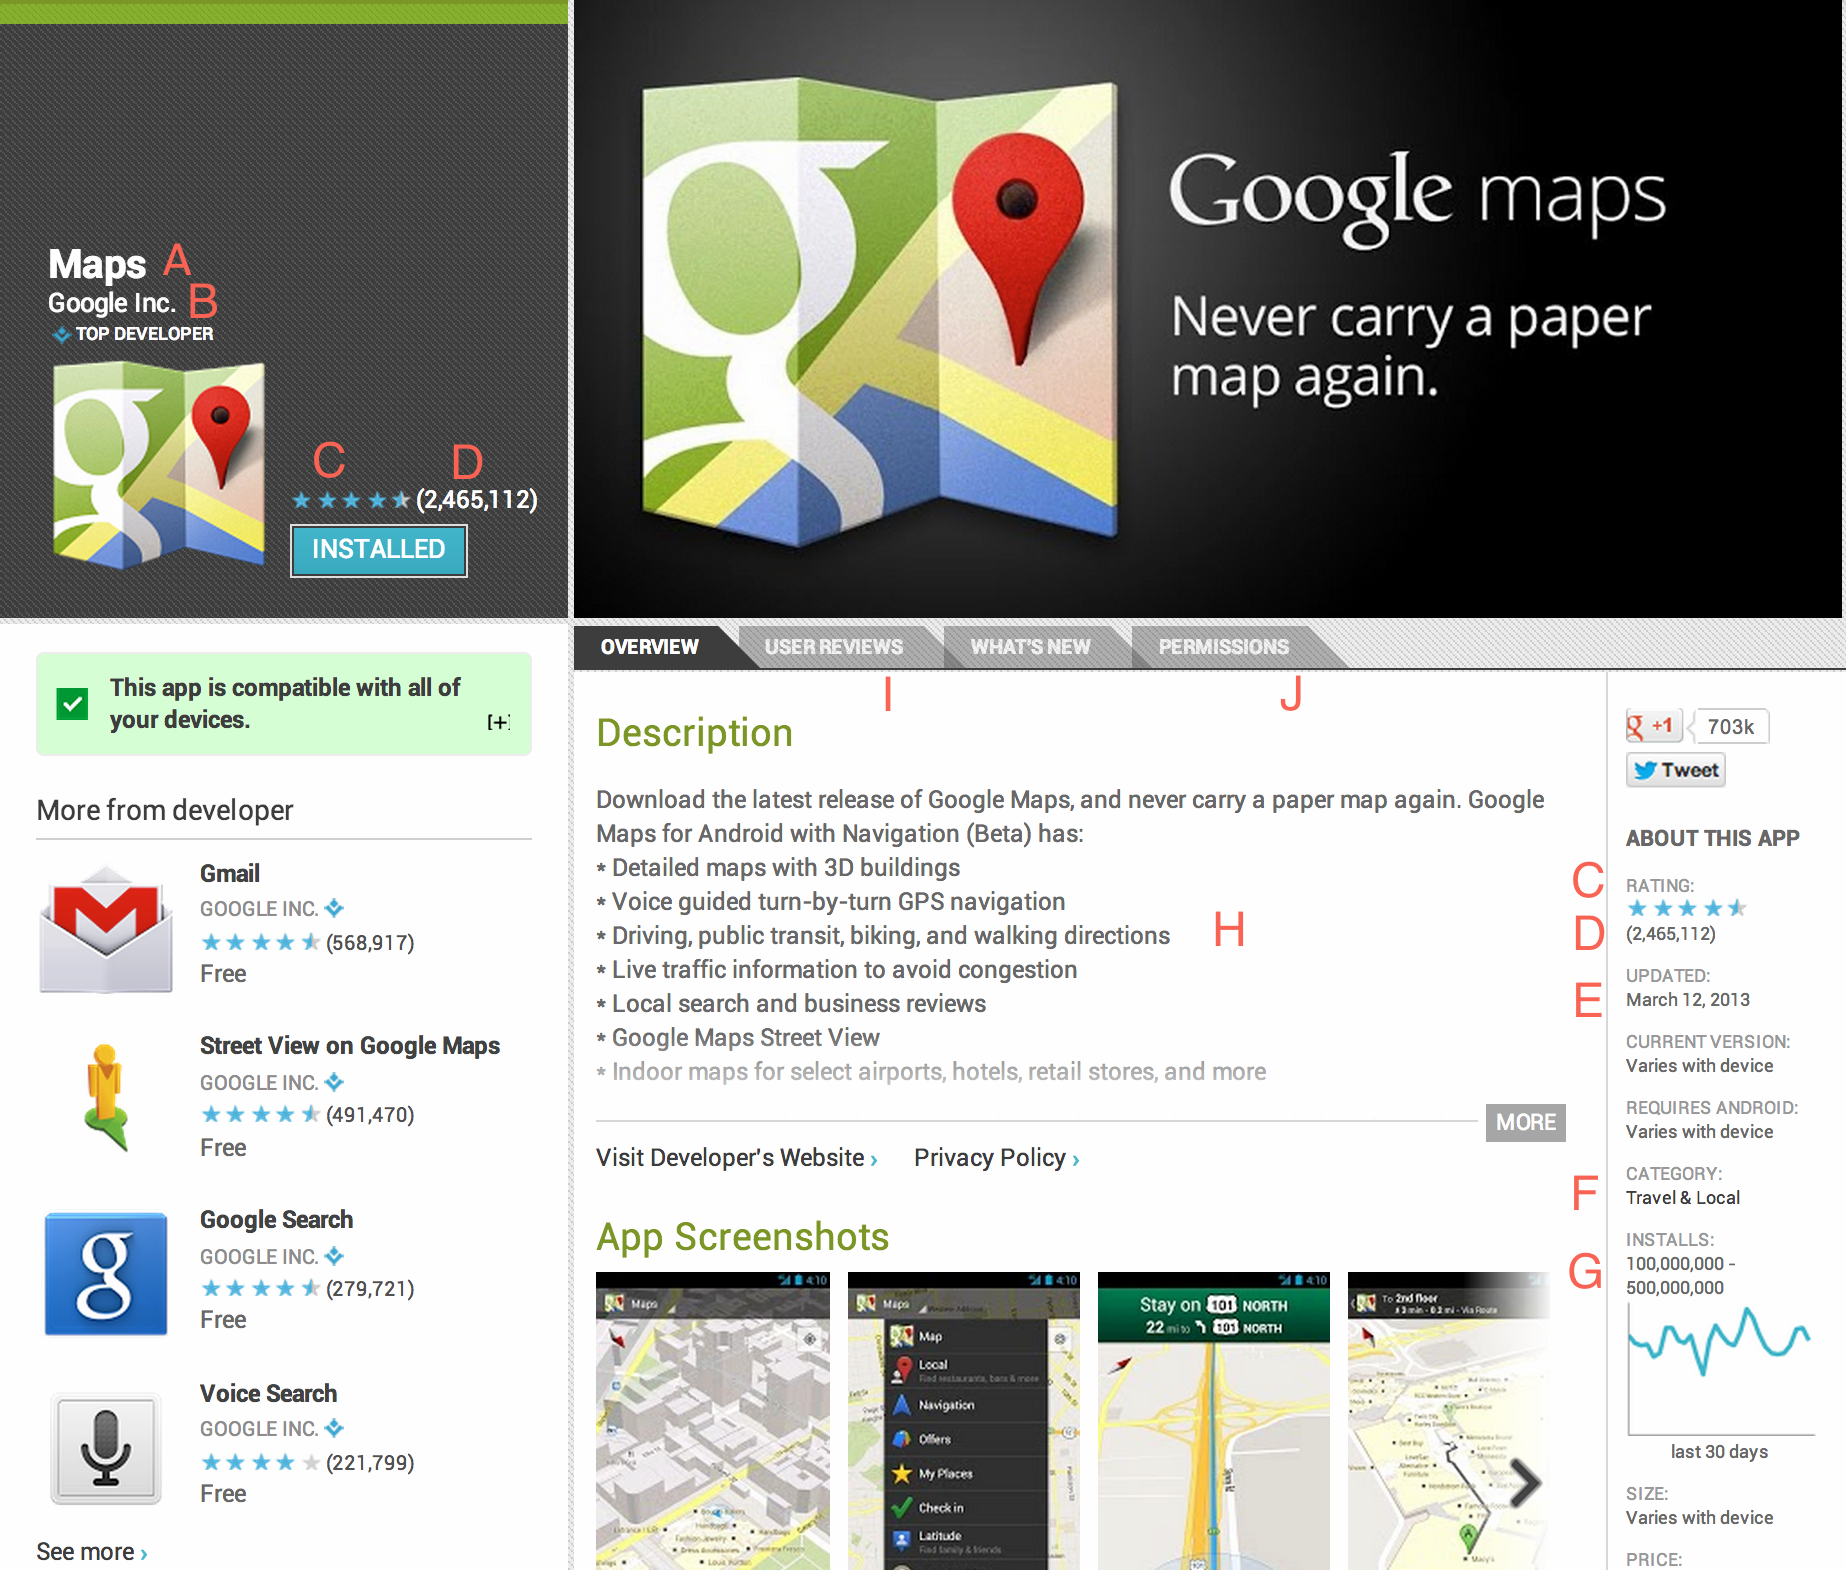
\includegraphics[width=0.9\columnwidth]{figs/GPStoreAppPage}
\caption{A sample page on the Google Play Store, see \ref{tab:gpstorekey}}
\label{fig:gpstoreapps}
\end{center}
\end{figure}

\begin{table*}[h]
\begin{small}
\begin{tabular}{l|l}

\textit{A} & App name  \\
\textit{B} & Developer Name  \\
\textit{C} & App Rating  \\
\textit{D} & Number of ratings  \\
\textit{E} & Date the app was last updated  \\
\textit{F} & Category in the Google Play Store it falls under  \\
\textit{G} & Number of installs (range, not exact number)  \\
\textit{H} & Description of the app  \\
\textit{I} & Reviews of the app  \\
\textit{J} & Permissions the app requests  \\

\end{tabular}
\end{small}
%\vspace{-0.2in}
\caption{Various properties of a Google Play Store app page}
\label{tab:gpstorekey}
%\vspace{-0.1in}
\end{table*}

%The core concept behind Android security - Permissions - are a static contract of capabilities. However, in this paper we propose an alternate means of conceptualizing security, which focuses on the interrelationship between the user's perception of the app, and the app's actual behavior. We call this the ``user-app agreement'', and will elaborate on it more later. 

\section{Malware}
Malware, as defined by the US Department of Homeland Security, is ``Short for malicious software. Programming (code, scripts, active content, and other software) designed to disrupt or deny operation, gather information that leads to loss of privacy or exploitation, gain unauthorized access to system resources, and other abusive behavior'' \citep{nash2005undirected}. Like PC OSs, malware is present on mobile OSs, although there are differences.


\subsection{Mobile Malware}
The tighter security model of Mobile OSs has a notable effect on mobile malware. With tight control in sandboxing, and app distribution, the usual viruses, trojans, and other exploits are more difficult to employ. The main vectors are either OS-level exploits, sneaking past the app review process, or through sideloading of apps. When looking at the two main mobile OSs, a stark contrast is shown. iOS has had  ``jailbreaking'' - privilege escalation exploits - dating back from it's first release \citep{damopoulos2011isam}, whereas the first Android exploit was not discussed until 2010 by security researchers Papathanasiou and Percoco \citep{papathanasiou2010not}, and was not seen in the wild until early 2011\citep{castillo2010android}. On the contrary, no side-loading is possible for iOS, and there have been very few - if any - instances of malware sneaking past Apple's App Store review process, although it has happened\footnote{In July 2012, SecureList noticed an iOS app that uploaded all of the user's contacts to a remote location without their consent\citep{SecureList2012}, but others argued this was not as devious as made out to be\citep{trendmicroios2012} }. With 95\% of all mobile malware\citep{nq2013}, Android's malware situation is very much a product of the sideloading and lack of review process found in GPStore\citep{nq2013}. %Of all the mobile malware found for iOS and Android, over \temp{some percent} used no system-exploits at all, \temp{some percent} on the main app distribution platform.

 On mobile devices, one of the dominant goals of malware is to gather information that leads to loss of privacy, found in over 28\% of mobile malware in 2012 alone\citep{nq2013}. This trend, of malware that possesses no system exploits, but gathers information that leads to loss of privacy, known as Info Theft Malware, is one that Android's Permission-based security model is ill-equipped to handle. Android's permission system relies on the user to determine at install-time if a list of capabilities should be entrusted with the given app. The user is not given a say in how or when the capabilities may be used, nor the ability to reject specific capabilities. At the same time, the mechanisms that keep mobile OSs safe are forcing malware writers to use more subtle techniques, often times without exploits. This all works against the user.

In this paper, we attempt to address this key issue through various means. We first introduce several novel concepts for analyzing apps and malware on Android. We then analyze the state of Android apps and Permissions with the most comprehensive android app database available, Android Census. Finally, we propose several novel improvements to the Android security architecture, called AndroMEDA, aimed at building off of our conceptual work.


\chapter{File System Architecture}
\label{sec:fs}

\begin{figure}[t]
\centerline{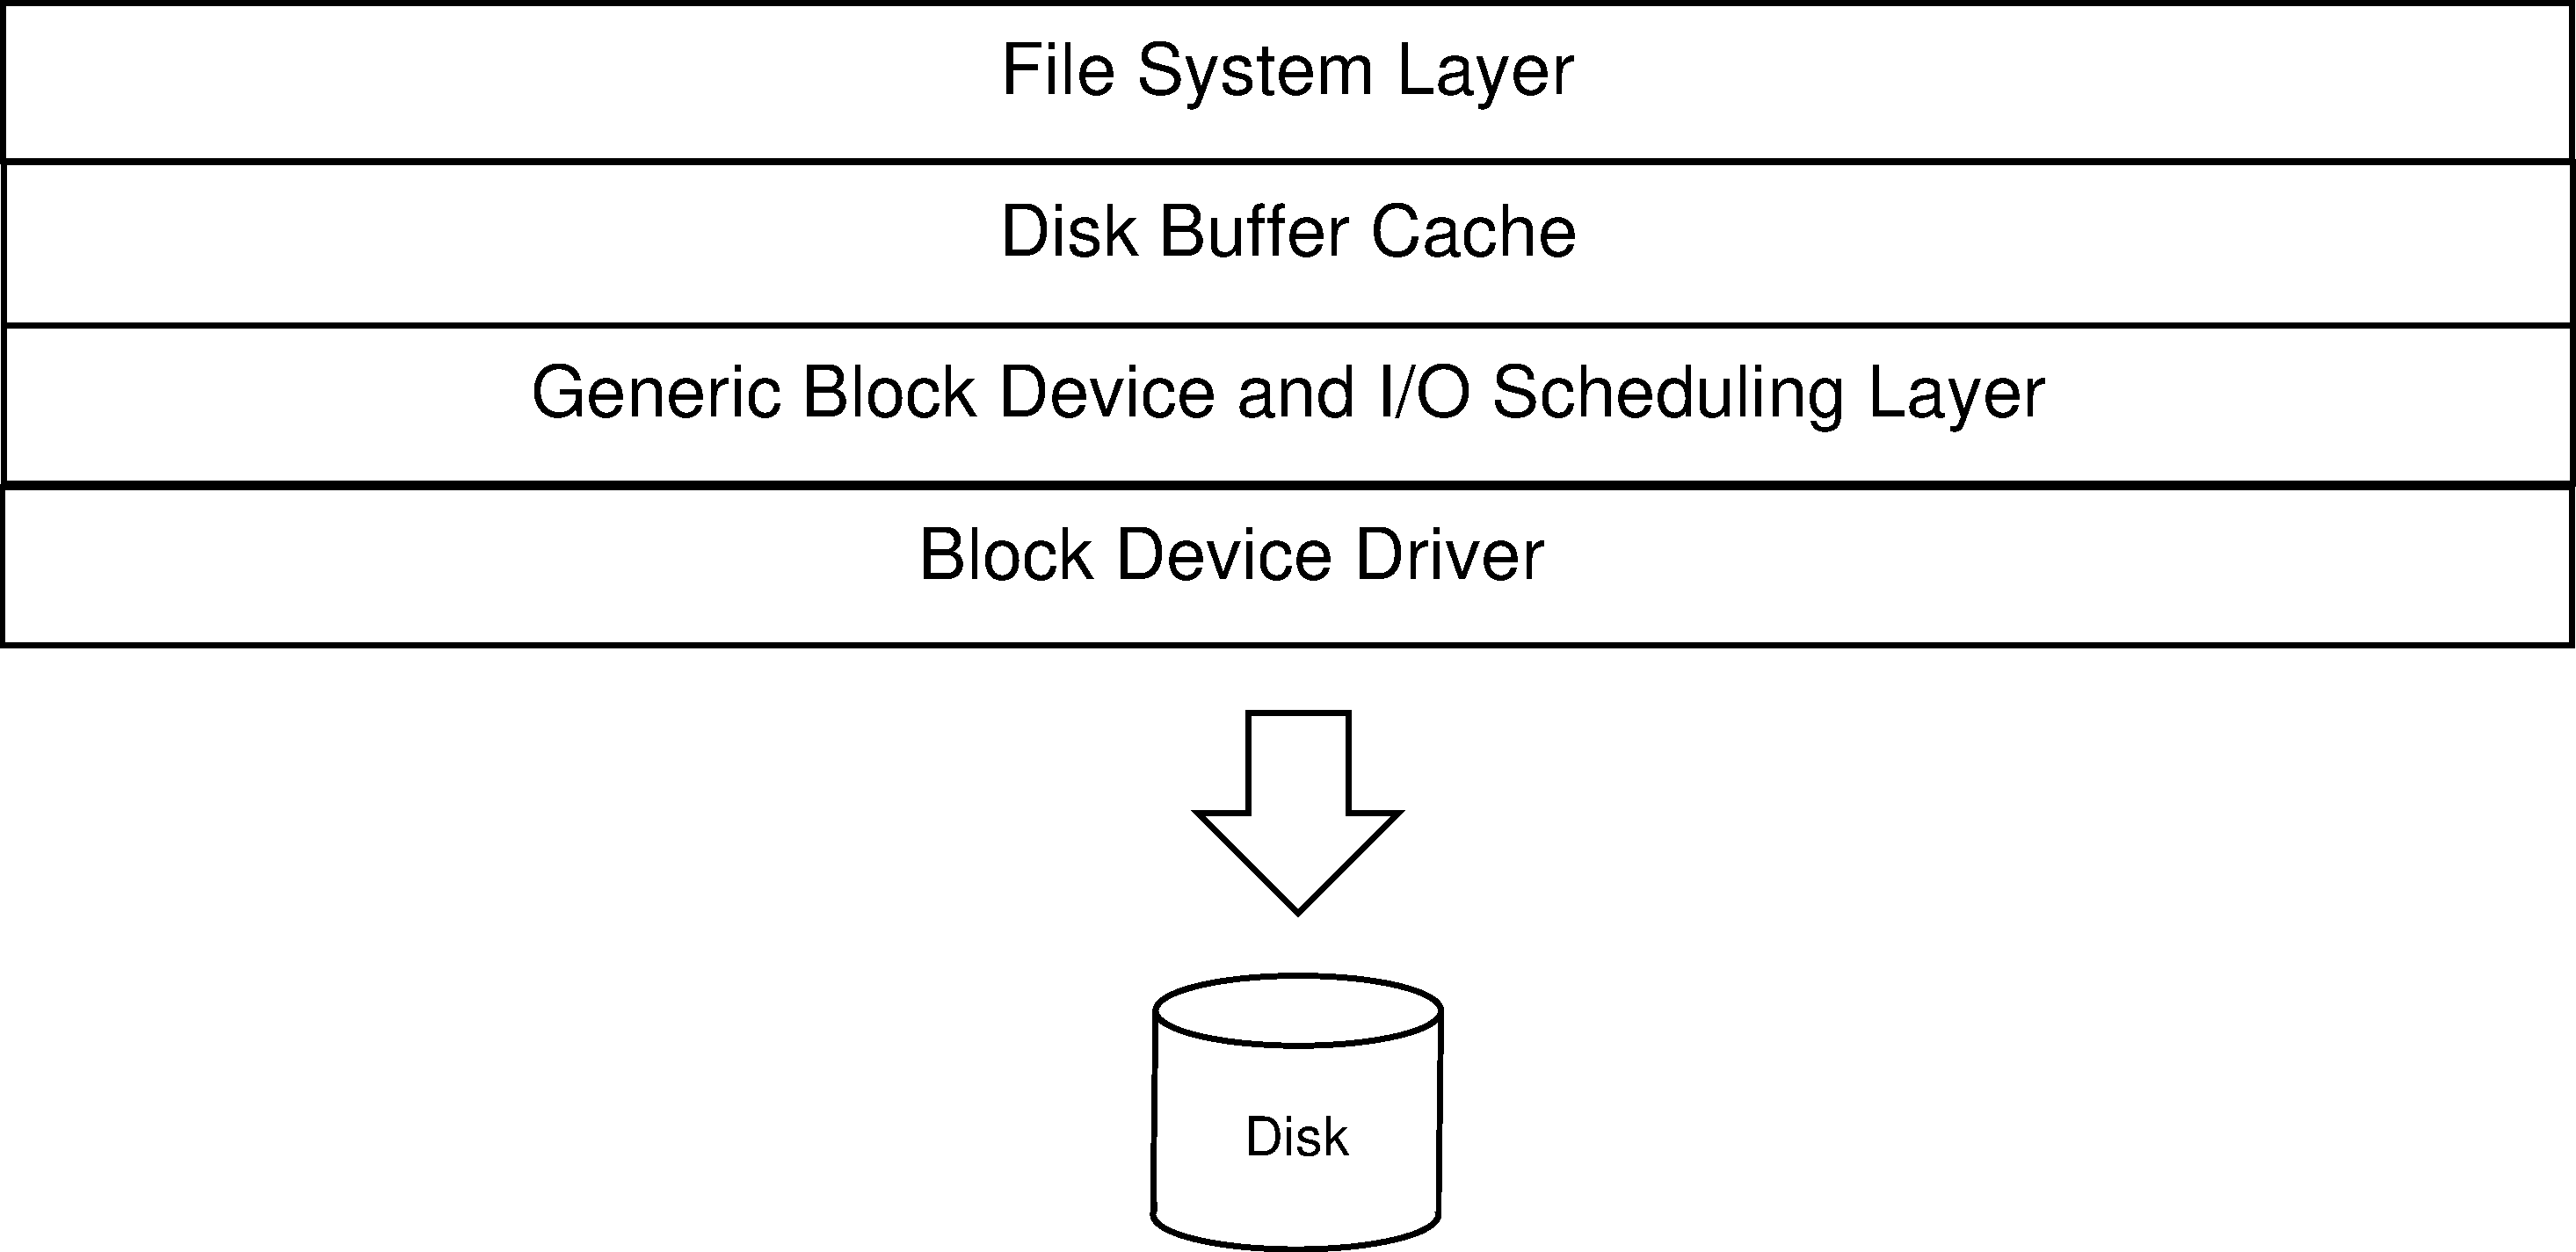
\includegraphics[width=0.7\columnwidth]{figs/block-fs-disk}}
\caption{File system architecture}
\label{fig:block-fs}
\end{figure}

Operating systems have traditionally provided support for persistent
storage through file systems. Files are read (or updated) by making
system calls which copy a region of memory from (or to) the
device. Introduced in the Multics input/output
system~\cite{Feiertag72}, the file interface is widely established and
is also used to access other devices like network cards in UNIX based
operating systems. The file system architecture in Linux is shown in
Figure~\ref{fig:block-fs}. Consider a write request for updating a
particular region of a file. First, the request passes through the
file system layer where changes to file system data structures like the
inode map are made. Then the updated pages are buffered in the disk
buffer cache. Pages marked as dirty in the disk buffer cache are then
periodically flushed to the block device layer, which is used to schedule
I/O operations for the hardware. The block device layer also supports
buffered I/O where a block of data can be read, modified and then
written back to the device. With the advent of non-volatile
byte-addressable memory, we believe that the overhead imposed by these
layers will be significant compared to the access latency for NVBM.

In order to measure the overhead at each layer, we perform an experiment where
a region of memory is updated in blocks of different sizes. Since NVBM is not
yet commercially available, we perform the experiments on DRAM, which has been
shown to be a good indicator of NVBM performance~\cite{Condit09}. All our
experiments were performed on a server with two Intel Xeon Quad-Core 2.67~GHz
(X5550) processors and 48~GB of 1333~MHz DDR3-RAM.  Each processor has 128~KB
L1, 256~KB L2, and 8~MB L3 caches. We used the Ubuntu~10.04 Linux distribution
and the 2.6.32-24 64-bit kernel.

\section{Direct Mapped Access}
For measuring the overhead at each layer, we use a direct mapped
experiment, where a region of memory is mapped into the application
and updates are performed directly on it, as a baseline. In the
baseline experiment there are no system calls invoked during the
updates. Updates of different sizes are performed using
\texttt{memcpy} and in order to ensure that there is no overhead due
to page faults, we first write to the entire region before beginning
the updates. The memory bandwidth obtained for different update sizes
is shown in Figure~\ref{fig:serial-large-block} and
Figure~\ref{fig:serial-small-block}. The memory bandwidth for direct
mapped access increases as the size of the updates increase from 1GB/s
for 2 byte updates to 9.1 GB/s for 128 byte updates. We believe this
is related to the number of bytes that can be transferred using one
SSE instruction.

\begin{figure}[t]
\begin{minipage}[b]{0.47\linewidth}
\centerline{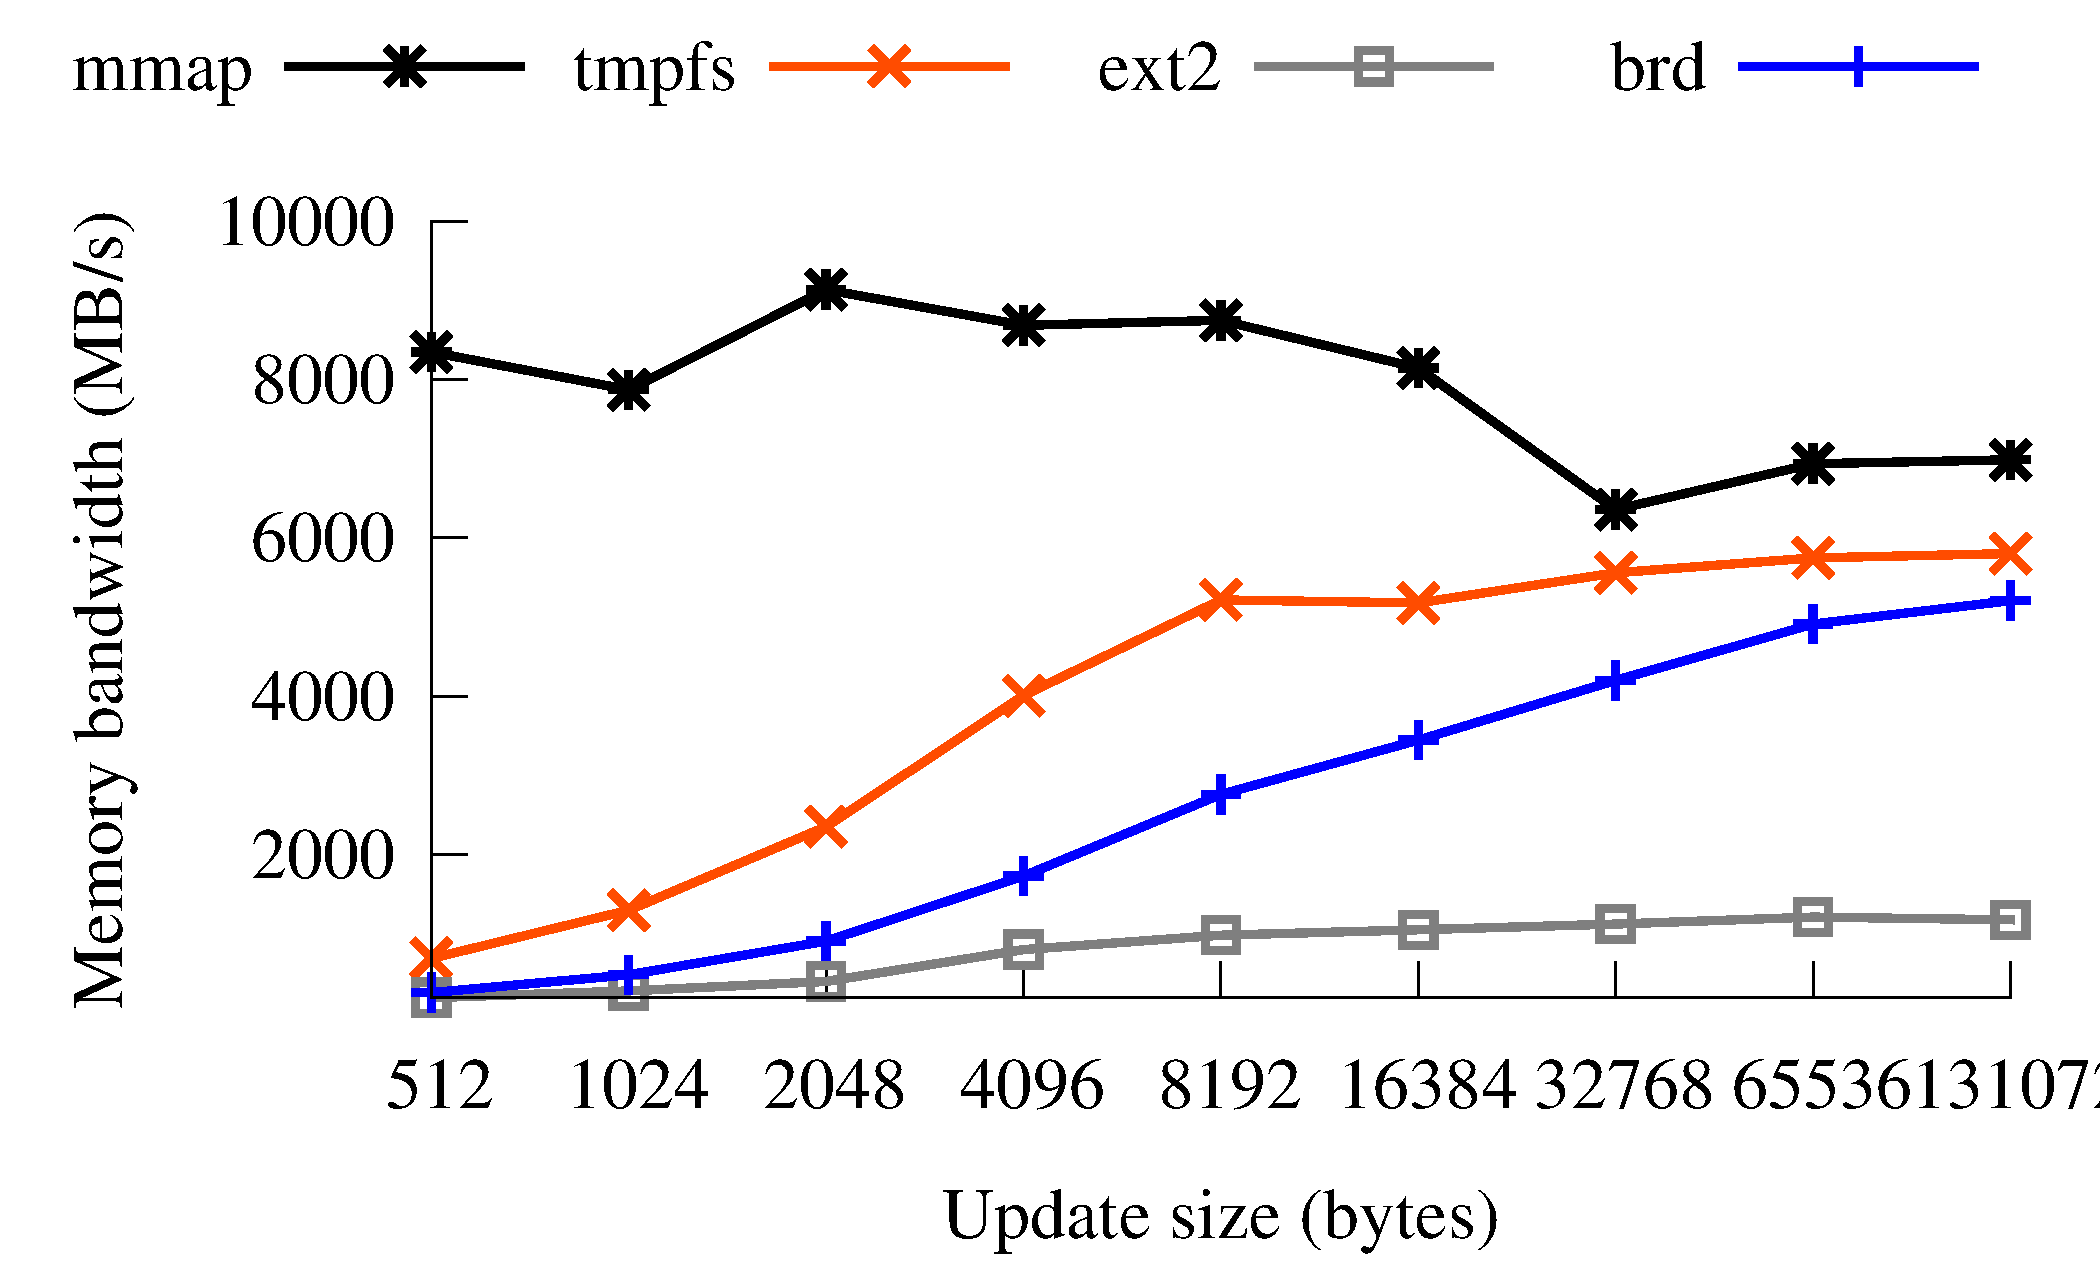
\includegraphics[width=\columnwidth]{figs/block-fs-large}}
\caption[Block device and File system overhead for large updates]
        {Block device and File system overhead for large updates. Note
         the linear scale on the y-axis}
\label{fig:serial-large-block}
\end{minipage}
\hspace{0.04\linewidth}
\begin{minipage}[b]{0.47\linewidth}
\centerline{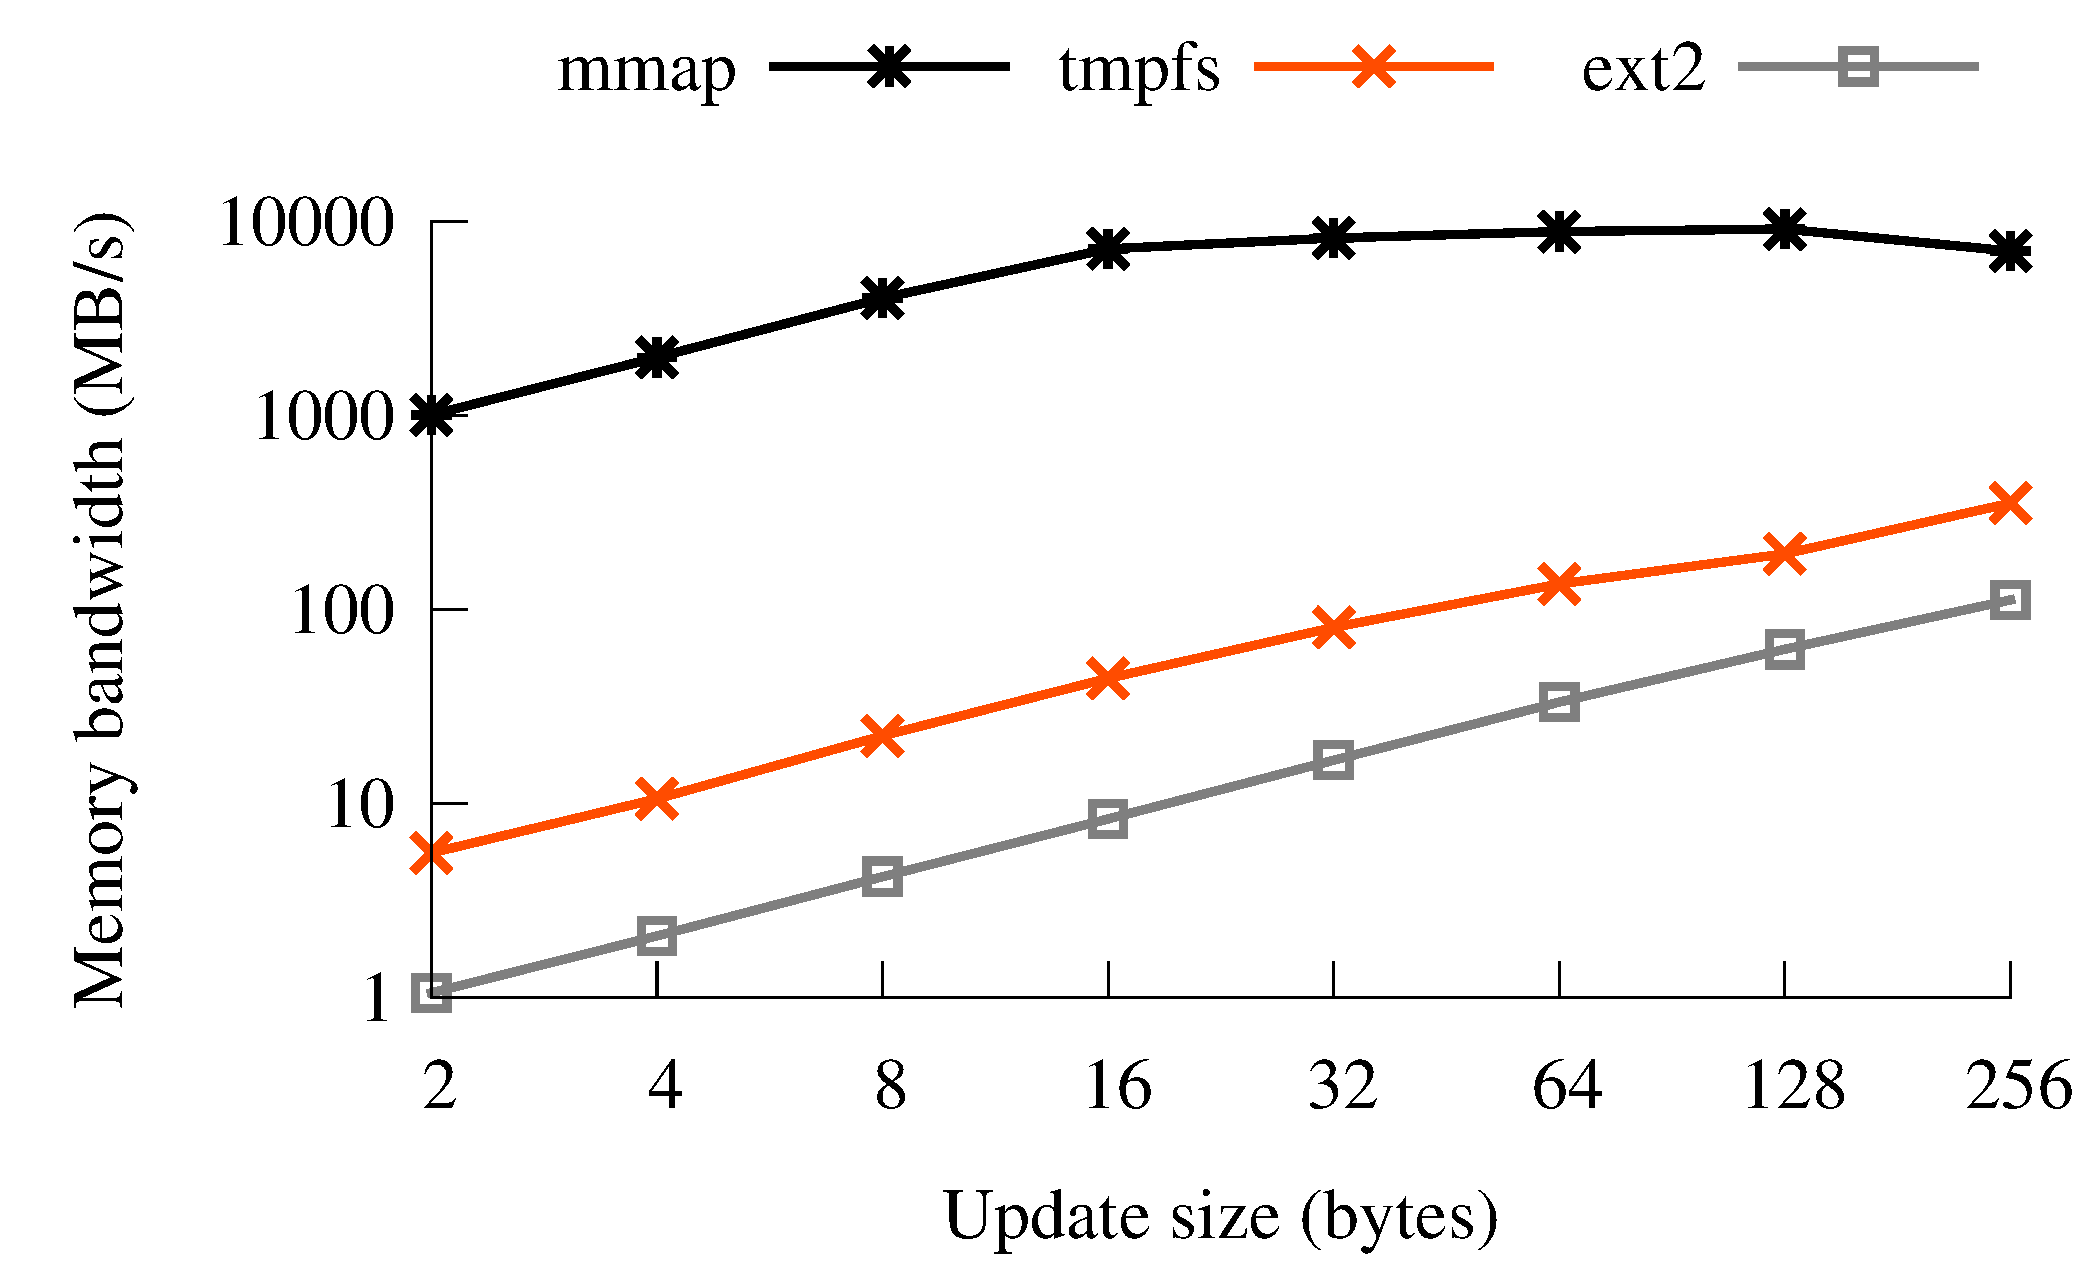
\includegraphics[width=\columnwidth]{figs/block-fs-small}}
\caption[Block device and File system overhead for small updates.]
        {Block device and File system overhead for small updates.  Note
        the log scale on the y-axis.}
\label{fig:serial-small-block}
\end{minipage}
%\vspace{-0.15in}
\end{figure}

\section{Block Device Layer}
To measure the overhead imposed by the block device layer, we measure
the performance of using the Block RAM device (BRD)~\cite{brd-linux}
to perform serial writes to a region of memory. The Block RAM device
in Linux exposes main memory as a block device and we perform updates
using write calls directly to the device, without mounting any
file system on it. Also in order to ensure that the writes are not
cached at the disk buffer cache, we open the device using the
O\_DIRECT flag. In this case, updates to the file are directly flushed
to the block device. The results presented in
Figure~\ref{fig:serial-large-block} show that as the block size is
varied between 512 bytes and 128KB, the overhead of using the block
device layer varies between $32$x and $1.3$x in terms of memory
bandwidth. (We were unable to perform updates smaller than 512 bytes
using O\_DIRECT as direct updates need to be multiples of the disk
sector size. This is another indication that the block device layer is
tuned for disks.)

\section{File Systems}
We consider two different configurations to demonstrate the overhead
of using a file system and correspondingly the file interface. First,
we mount ext2 on BRD and measure the time required to perform serial
writes to a file. The results shown in
Figure~\ref{fig:serial-small-block} show that mounting ext2 on BRD
performs worse than writing directly to the device. This is due to the
additional overhead of the file system layer which is combined with
that of the block device interface.

We also considered \texttt{tmpfs}~\cite{tmpfs} an in-memory file
system in Linux, where the data is stored in the page cache. As a
result, there is no block device overhead in this case and we can
measure the overhead of the file system layer. The results shown in
Figure~\ref{fig:serial-small-block} show that for smaller 64B block sizes,
direct mapped access is $65$ times faster than using
\texttt{tmpfs}. However as the block size is increased to 4K, we find
that the performance converges to within 83\% of direct mapped
access.

\begin{figure}[t!]
\begin{minipage}[b]{0.45\linewidth}
\centerline{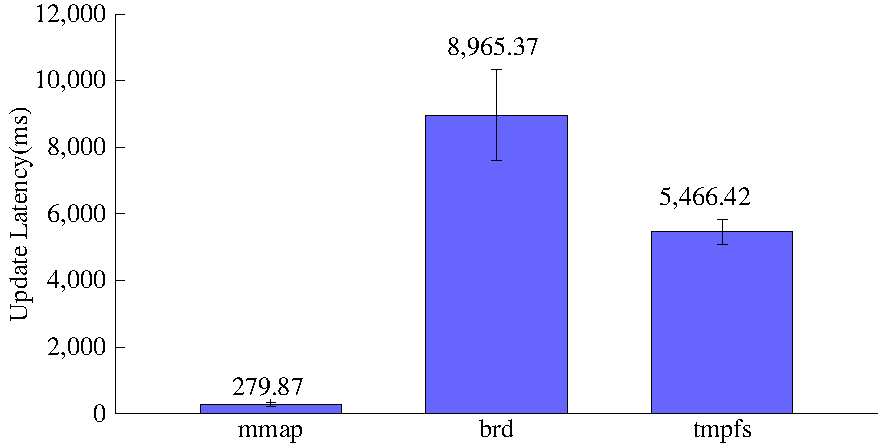
\includegraphics[width=\columnwidth]{figs/flush-fs}}
\caption{Latency for cache line sized update and flush}
\label{fig:random-update}
\end{minipage}
\hspace{0.04\linewidth}
\begin{minipage}[b]{0.45\linewidth}
\begin{center}
\begin{tabular}{cc}
\toprule
System & No. of function calls \\
\midrule
tmpfs & 64 \\
Block RAM Device (BRD) & 136 \\
ext2 on BRD  & 192 \\
\bottomrule
\end{tabular}
\captionof{table}{Number of kernel functions invoked in one \texttt{sys\_write} system call}
\label{tab:syscall}
\end{center}
\end{minipage}
\end{figure}

\section{Flush Overhead}
Since NVBM will be available through DIMM slots, we can flush cache line
sized updates to the device. However the block device and the
file system layer can only flush updates which are equal to the page
size (4KB in Linux). We performed an experiment to measure the
overhead due to this limitation. In this experiment, we create a file
of a fixed size and seek to a random location in the file. We then
perform a cache line sized update and flush the update to NVBM using the
\texttt{fsync} call. The Block RAM device and \texttt{tmpfs} layers were
modified to invoke the \texttt{clflush} instruction for a sync
operation. We compare the time taken against performing
\texttt{clflush} from a userspace application. The results of this
experiment are shown in Figure~\ref{fig:random-update}. The time taken
to update and flush a cache line is around 280ns from the userspace
application. When compared to direct mapped access, the latency
of using \texttt{tmpfs} and the Block RAM device is greater by $19.5$x
and $32$x respectively. 
% There are some possible additional issues like the granularity of
% transactions and coordination at  a block level is inefficient -
% False sharing. Reading large chunks of file systems into memory causes
% large number of cache invalidations and cache use overhead - NVBM would
% allow finer grain access control (cf files or databases), far less false
% sharing for shared data, and far less cache invalidations for
% shared data, and far less cache invalidations for applications that are
% only doing partial updates on files

\section{System Call Overhead}
In addition to measuring the memory bandwidth and latencies, we profiled the
kernel functions invoked for every system call using LTTng~\cite{lttng}, a
Linux-kernel tracing tool. The number of function calls invoked for a single
\texttt{sys\_write} system call for \texttt{tmpfs}, BRD and ext2 on BRD is
shown in Table~\ref{tab:syscall}. While the system call implementations have
been optimized over the years, their performance will always be slower than
performing no system calls at all.  Hence, providing direct mapped access to
NVBM removes the operating system from the critical path and overcomes any
overheads for performing reads and writes.  However, the OS will play in
important role in providing isolation for directly mapped pages and
we discuss issues related to safety in Chapter~\ref{sec:conclusion}.

\chapter{Design and Implementation}
\label{sec:design}

As mentioned previously, we expect NVBM to be exposed across a memory bus and
not via a legacy disk interface.  In addition to the file system and block
device overhead measured in Chapter~\ref{sec:fs}, using the PCI interface
(256~ns latency~\citep{Holden06}) or even a kernel-based syscall API (89.2 and
76.4~ns for POSIX \texttt{read/write}) would add significant overhead to NVBM's
access latencies (50--150~ns).  As shown in Chapter~\ref{sec:fs}, the overhead
of using file systems or buffered updates would also be prohibitively large.
Further, given the performance and energy cost of moving data, we believe that
all data should reside in a single-level store where no distinction is made
between volatile and persistent storage and all updates are performed in-place.
We therefore propose that data access should use userspace libraries and APIs
that map data into the process's address space.

However, the same properties that allow systems to take full advantage
of NVBM's performance properties also introduce challenges.  In
particular, one of the biggest obstacles is that current processors do
not provide primitives to order memory writes.  Combined with the fact
that the memory controller can reorder writes (at a cache line
granularity), current mechanisms for updating data structures are
likely to cause corruption in the face of power or software failures.
For example, assume that a hash table insert requires the write of a
new hash table object and is followed by a pointer write linking the
new object to the hash table.  A reordered write could propagate the
pointer to main memory before the object and a failure at this stage
would cause the pointer to link to an undefined memory region.
Processor modifications for ordering can be complex~\citep{Condit09},
do not show up on vendor roadmaps, and will likely be preceded by NVBM
availability.

To address these issues, our design and implementation focuses on
three different layers. First, in Chapter~\ref{sec:flush}, we describe
how we implement ordering and flushing of data on existing processors.
However, this low-level primitive is not sufficient for atomic updates
larger than 8~bytes.  In addition, we therefore also require 
versioning CDDSs, whose design principles are described in
Chapter~\ref{sec:cdds_overview}.  After discussing our CDDS B-Tree
implementation in Chapter~\ref{sec:cdds_btree} and some of the open
opportunities and challenges with CDDS data structures in
Chapter~\ref{sec:cdds_discuss}, Chapter~\ref{sec:kv} describes Tembo,
the system resulting from the integration of our CDDS B-Tree into a
distributed Key-Value system.

\section{Flushing Data on Current Processors}
\label{sec:flush}

As mentioned earlier, today's processors have no mechanism for
preventing memory writes from reaching memory and doing so for
arbitrarily large updates would be infeasible.  Similarly, there is no
guarantee that writes will not be reordered by either the processor or
by the memory controller.  While processors support a \texttt{mfence}
instruction, it only provides write visibility and does not guarantee
that all memory writes are propagated to memory (NVBM in this case) or
that the ordering of writes is maintained.  While cache contents can
be flushed using the \texttt{wbinvd} instruction, it is a
high-overhead operation (multiple ms per invocation) and flushes the
instruction cache and other unrelated cached data.  While it is
possible to mark specific memory regions as write-through, this impacts
write throughput as all stores have to wait for the data to reach main
memory.


To address this problem, we use a combination of tracking recently
written data and use of the \texttt{mfence} and \texttt{clflush}
instructions.  \texttt{clflush} is an instruction that invalidates the
cache line containing a given memory address from all levels of the
cache hierarchy, across multiple processors.  If the cache line is dirty
(i.e., it has uncommitted data), it is written to memory before
invalidation. The \texttt{clflush} instruction is also ordered by the
\texttt{mfence} instruction.
%\footnote{Instructions available on Intel and AMD CPUs since 2000 and 2003.}
Therefore, to commit a series of memory writes, we first execute an
\texttt{mfence} as a barrier to them, execute a \texttt{clflush} on
every cacheline of all modified memory regions that need to be
committed to persistent memory, and then execute another
\texttt{mfence}.  In this paper, we refer to this instruction
sequence as a \textit{\texttt{flush}}.  As microbenchmarks in
Chapter~\ref{sec:flush_perf} show, using \texttt{flush} will be
acceptable for most workloads.

While this description and tracking dirty memory might seem complex,
this was easy to implement in practice and can be abstracted away by
macros or helper functions.  In particular, for data structures, all
updates occur behind an API and therefore the process of
\texttt{flush}ing data to non-volatile memory is hidden from the
programmer. Using the simplified hash table example described above,
the implementation would first write the object and \texttt{flush}
it. Only after this would it write the pointer value and then
\texttt{flush} again.  This two-step process is transparent to the
user as it occurs inside the insert method.

Finally, one should note that while \texttt{flush} is necessary for
durability and consistency, it is not sufficient by itself.  If any
metadata update (e.g., rebalancing a tree) requires an atomic update
greater than the 8~byte atomic write provided by the hardware, a
failure could leave it in an inconsistent state.  We therefore need
the versioning approach described below in Chapters~\ref{sec:cdds_overview}
and~\ref{sec:cdds_btree}.

\section{CDDS Overview}
\label{sec:cdds_overview}

Given the challenges highlighted at the beginning of
Chapter~\ref{sec:design}, an ideal data store for non-volatile memory
must have the following properties:

\begin{smitemize}
\item \textbf{Durable}: The data store should be durable.  A fail-stop
  failure should not lose committed data.

\item \textbf{Consistent}: The data store should remain consistent
  after every update operation. If a failure occurs during an update,
  the data store must be restored to a consistent state before further
  updates are applied.

\item \textbf{Scalable}: The data store should scale to
  arbitrarily-large sizes.  When compared to traditional data stores,
  any space, performance, or complexity overhead should be minimal.

\item \textbf{Easy-to-Program}: Using the data store should not
  introduce undue complexity for programmers or unreasonable
  limitations to its use.

\end{smitemize}


\begin{figure*}[tbh]
\centerline{
\begin{tikzpicture}[scale=0.75, transform shape]
\begin{scope}
[level 1/.style={sibling distance=8.5cm},
 level 2/.style={sibling distance=3.3cm}]
[node distance=2cm on grid, >=stealth', auto]
 \node[nd={d,l,l}] {
    \btnode{text}{99}{1}{6}
    \btnode{second}{99}{6}{-}
 }
 child {node[nd={d,d,d}] (b1) {
    \btnode{text}{20}{4}{6}
    \btnode{second}{99}{1}{4}
    \btnode{third}{99}{4}{6}
   }
   child{node[nd={d,d,d}] (c2) {
       \btnode{text}{5}{4}{6}
       \btnode{second}{10}{5}{6}
       \btnode{third}{20}{4}{6}
       }
   }
   child{node[nd={d,d,d}] (c1) {
       \btnode{text}{5}{2}{4}
       \btnode{second}{20}{3}{4}
       \btnode{third}{99}{1}{4}
       }
   }
   child{node[nd={l,l,l}] (c3) {
       \btnode{text}{40}{4}{-}
       \btnode{second}{99}{4}{-}
       }
   }
 }
 child [parent anchor = south] {node[nd={l,l,l}] (b2) {
    \btnode{text}{10}{6}{-}
    \btnode{second}{20}{6}{-}
    \btnode{third}{99}{6}{-}
   } 
   child [parent anchor = one south] {node[nd={l,l,l}] {
       \btnode{text}{5}{6}{-}
       \btnode{second}{8}{7}{-}
       \btnode{third}{10}{6}{-}
     }
   }
   child [parent anchor = south]{node[nd={l,d,l}] {
       \btnode{text}{13}{9}{-}
       \btnode{second}{15}{6}{8}
       \btnode{third}{20}{6}{-}
     }
   }
 };
 \draw [-] (b2.three south) to  (c3.north); 
\end{scope}
\begin{scope}[xshift=9cm, yshift=-1.75cm, node distance=4mm]
\node (live) [rectangle, thick, draw=black!75, inner sep=4mm, 
              label=right:Live entry] {\\};
\node (dead) [below =of live, thick, draw=black!75, fill=black!25,
              inner sep=4mm, label=right:Dead entry] {\\};
\end{scope}
\begin{scope}[xshift=9.5cm]
\node [rectangle, thick, draw=black!75, inner sep=1mm,% font=\large,
       align=center]{
{\small $Key$}\\
$\left[ {Start \atop Version} , {End \atop Version} \right)$
%% $
%% \left( \begin{array}{c@{,}c}
%% Start & End \\
%% Version & Version
%% \end{array}
%% \right)
%% $
%% \begin{tabular}{cc}
%%   \multicolumn{2}{c}{Key} \\
%%   Start & End \\
%%   Version & Version
%% \end{tabular}
};
%       align=center]{ Key \\ $[$start, end$)$ };
\end{scope}
\end{tikzpicture}
}
%\vspace{-0.1in}
\caption{Example of a CDDS B-Tree}
\label{fig:cd-btree}
%\vspace{-0.15in}
\end{figure*}

We believe it is possible to meet the above properties by storing data
in Consistent and Durable Data Structures (CDDSs), i.e., hardened
versions of conventional data structures currently used with volatile
memory.  The ideas used in constructing a CDDS are applicable to a
wide variety of linked data structures and, in this paper, we
implement a CDDS B-Tree because of its non-trivial implementation
complexity and widespread use in storage systems.  We would like to
note that the design and implementation of a CDDS only addresses
\textit{physical} consistency, i.e., ensuring that the data structure
is readable and never left in a corrupt state.  Higher-level layers
control \textit{logical} consistency, i.e., ensuring that the data
stored in the data structure is valid and matches external integrity
constraints.  Similarly, while our current system implements a simple
concurrency control scheme, we do not mandate concurrency control to
provide isolation as it might be more efficient to do it at a higher
layer.

A CDDS is built by maintaining a limited number of versions of the
data structure with the constraint that an update should not weaken
the structural integrity of an older version and that updates are
atomic.  This versioning scheme allows a CDDS to provide consistency
without the additional overhead of logging or shadowing.  A CDDS thus
provides a guarantee that a failure between operations will never
leave the data in an inconsistent state.  As a CDDS never acknowledges
completion of an update without safely committing it to non-volatile
memory, it also ensures that there is no silent data loss.



\section{Versioning for Durability}
\label{sec:versioning_overview}

Internally, a CDDS maintains the following properties:

\begin{smitemize}
  \item There exists a version number for the most recent consistent
    version.  This is used by any thread which wishes to read from the
    data structure.
  \item Every update to the data structure results in the creation of
    a new version.
  \item During the update operation, modifications ensure that existing 
    data contained in older versions is never overwritten. Such
    modifications are performed by either using atomic operations
    or copy-on-write style changes.
  \item After all the modifications for an update have been made
    persistent, the most recent consistent version number is updated
    atomically and the operation is committed .
\end{smitemize}


\subsection{Garbage Collection}

Along with support for multiple versions, a CDDS also tracks versions
of the data structure that are being accessed.  Knowing the oldest
version which has a non-zero reference count has two benefits.  First,
we can garbage collect older versions of the data structure. Garbage
collection (GC) is run in the background and helps bound the space
utilized by eliminating data that will not be referenced in the
future.  Second, knowing the oldest active version can also improve
performance by enabling intelligent space reuse in a CDDS\@. When
creating a new entry, the CDDS can proactively reclaim the space used
by older inactive versions.



\subsection{Failure Recovery}

Insert or delete operations may be interrupted due to operating system
crashes or power failures.  By definition, the most recent consistent
version of the data structure should be accessible on recovery.
However, an in-progress update needs to be removed as it belongs to an
uncommitted version.  We handle failures in a CDDS by using a `forward
garbage collection' procedure during recovery.  This process involves
discarding all update operations which were executed after the most
recent consistent version.  Newly created entries can be discarded while
older entries with in-progress update operations are reverted.

% The recovery procedure is closely related to the
% concurrency model used. The currently implemented shared reader,
% single writer concurrency model enables fast and simple recovery.

%\begin{figure*}[tbh]
%  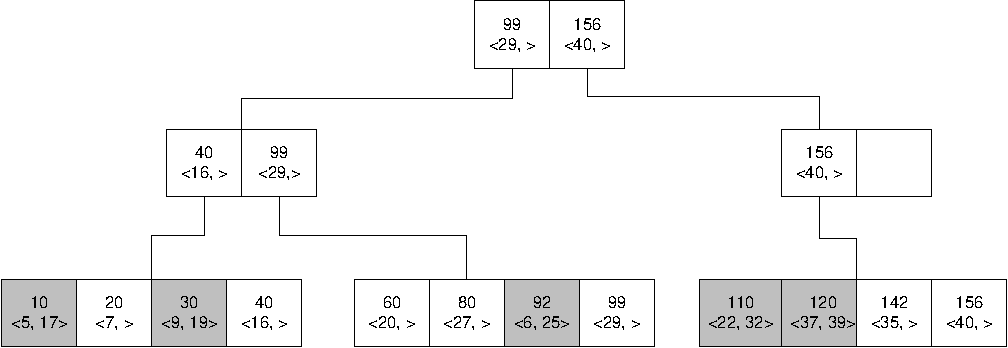
\includegraphics[width=\textwidth]{figs/cd-btree}
%  \caption{Example of a Consistent and Durable B-Tree}
%  \label{fig:cd-btree} 
%\end{figure*}


\section{CDDS B-Trees}
\label{sec:cdds_btree}

As an example of a CDDS, we selected the B-Tree~\citep{Comer79} data
structure because of its widespread use in databases, file systems,
and storage systems.  This section discusses the design and
implementation of a consistent and durable version of a B-Tree.  Our
B-Tree modifications\footnote{In reality, our B-Tree is a B+~Tree with
  values only stored in leaves.} have been heavily inspired by
previous work on multi-version data
structures~\citep{Becker96,Varman97}.  However, our focus on
durability required changes to the design and impacted our
implementation.  We also do not retain all previous versions of the
data structure and can therefore optimize updates.

In a CDDS B-Tree node, shown in Figure~\ref{fig:cd-btree}, the key and
value stored in a B-Tree entry is augmented with a start and end
version number, represented by unsigned 64-bit integers.  A B-Tree
node is considered `live' if it has at least one live entry.  In turn,
an entry is considered `live' if it does not have an end version
(displayed as a `$-$' in Figure~\ref{fig:cd-btree}). To bound space utilization, in
addition to ensuring that a minimum number of entries in a B-Tree node
are used, we also bound the minimum number
of live entries in each node.  Thus, while the CDDS B-Tree API is
identical to normal B-Trees, the implementation differs
significantly.
In the rest of this section, we use the \textit{lookup},
\textit{insert}, and \textit{delete} operations to illustrate how the
CDDS B-Tree design guarantees consistency and durability.
%\footnote{A longer
%  technical report~\citep{Venkataraman10} presents more
%  details on all CDDS B-Tree operations and their corresponding
%  implementations.}.


\subsection{Lookup}
\label{sec:btree_lookup}

We first briefly describe the lookup algorithm, shown in 
Algorithm~\ref{alg:btree_lookup}.  For ease of explanation,
the pseudocode in this and following algorithms does not
include all of the design details.  The algorithm uses the
\texttt{find} function to recurse down the tree
(lines~\ref{line:l_descend}--\ref{line:l_descend_done}) until it finds
the leaf node with the correct key and value.

\begin{algorithm}[t]
\dontprintsemicolon
\linesnumbered

\SetAlFnt{\sf}
\SetAlCapFnt{\sf}

\SetKwFunction{GetLastConsistentVersion}{get\_last\_consistent\_version}
\SetKwFunction{GetNumEntries}{get\_num\_entries}
\SetKwFunction{NumLiveEntries}{num\_live\_entries}
\SetKwFunction{Insert}{insert}
\SetKwFunction{IsInnerNode}{is\_inner\_node}
\SetKwFunction{Lookup}{lookup}
\SetKwFunction{Find}{find}

\KwIn{k: key, r: root}
\KwOut{val: value}
\Begin(\Lookup{k, r}){
    $v \leftarrow  current\_version$\; \nllabel{line:l_version}
    $n \leftarrow r$\;
    \While { \IsInnerNode{n} } {  \nllabel{line:l_descend}
      $entry\_num \leftarrow \Find{k, n, v}$\; 
      $n \leftarrow n[entry\_num].child$\; \nllabel{line:l_descend_done}
    }
    $entry\_num \leftarrow \Find{k, n, v}$\; 
    \Return{$n[entry\_num].value$}\;
}
\BlankLine
\Begin(\Find{k, n, v}) {
  $l \leftarrow 0$\;
  $h \leftarrow \GetNumEntries{n}$\;
  \While(\tcp*[f]{Binary Serch}) { $l < h$ } { \nllabel{line:l_binary}
    $m \leftarrow (l + h)/2$\;
    \If { $k \leq n[m].key$ } {
      $h \leftarrow m-1$\;
    } \lElse $l \leftarrow m+1$\;   \nllabel{line:l_binary_done}
  }
  \While { $h < \GetNumEntries {n}$ } { \nllabel{line:vcheck}
    \If { $n[h].start \leq v$ } {
      \If { $n[h].end > v \quad \| \quad n[h].end = 0$ } {
        $break$\;
      }
    }
    $h \leftarrow h+1$\;  \nllabel{line:vcheck_done}
  }
  \Return{$h$}\;
}
\caption{CDDS B-Tree Lookup}
\label{alg:btree_lookup}
\end{algorithm}


Consider a lookup for the key $10$ in the CDDS B-Tree shown in
Figure~\ref{fig:cd-btree}.  After determining the most current version
(version $9$, line~\ref{line:l_version}), we start from the root node
and pick the rightmost entry with key $99$ as it is the next largest
valid key.  Similarly in the next level, we follow the link from the
leftmost entry and finally retrieve the value for $10$ from the leaf
node.

Our implementation currently optimizes lookup performance by ordering
node entries by key first and then by the start version number.
This involves extra writes during inserts to shift entries but
improves read performance by enabling a binary search within nodes
(lines~\ref{line:l_binary}--\ref{line:l_binary_done} in
\texttt{find}).  While we have an alternate implementation that
optimizes writes by not ordering keys at the cost of higher lookup
latencies, we do not use it as our target workloads are
read-intensive.  Finally, once we detect the right index in the node,
we ensure that we are returning a version that was valid for $v$, the
requested version number
(lines~\ref{line:vcheck}--\ref{line:vcheck_done}).


\begin{algorithm}[t]
\dontprintsemicolon
\linesnumbered

\SetAlFnt{\sf}
\SetAlCapFnt{\sf}

\SetKwFunction{GetLastConsistentVersion}{get\_last\_consistent\_version}
\SetKwFunction{GetNumEntries}{get\_num\_entries}
\SetKwFunction{SetNumEntries}{set\_num\_entries}
\SetKwFunction{CanReuseVersion}{can\_reuse\_version}
\SetKwFunction{SplitInsert}{split\_insert}
\SetKwFunction{Flush}{flush}
\SetKwFunction{InsertKey}{insert\_key}
\SetKwFunction{NumLiveEntries}{num\_live\_entries}
\SetKwFunction{MinLiveEntries}{min\_live\_entries}
\SetKwFunction{Insert}{insert}
\SetKwFunction{NewNode}{new\_node}

\KwIn{k: key, r: root}
\Begin(\InsertKey{k, r}){
    $v \leftarrow current\_version$\; \nllabel{line:i_version1}
    $v'\leftarrow v+1$\; \nllabel{line:i_version2}
    \tcp{Recurse to leaf node (n)}\;
    %\vdots\;
    %\BlankLine
    $y \leftarrow \GetNumEntries{n} $\;
    \If(\tcp*[f]{Node Full}){$y = node\_size$} {  \nllabel{line:i_full}
      \If {entry\_num = \CanReuseVersion{$n, y$}}{
        \tcp{ Remove the oldest entry }
        %      (again maintaining sorted order)
        % \BlankLine
        % \tcp{ Insert in sorted order} 
        $n[entry\_num].key \leftarrow k $\;
        $n[entry\_num].start \leftarrow v' $\;
        $n[entry\_num].end \leftarrow 0 $\;
        \Flush{$n[entry\_num]$} \; \nllabel{line:i_nslot_flush}\;
      }
      \Else {
        \SplitInsert{$n$, $k$, $v'$}\;
        %\BlankLine
        \tcp{Update inner nodes}\;
      }
    }
    \Else{
      $n[y].key \leftarrow k $\;
      $n[y].start \leftarrow v' $\;
      $n[y].end \leftarrow 0 $\;
      \Flush{$n[y]$} \; \nllabel{line:i_ny_flush}\;
    }
%   XXX - Too confusing. What about split nodes? In that case n is
%   invalid.
%    \SetNumEntries{$n$, $y+1$}\;
    $current\_version \leftarrow v'$\; \nllabel{line:i_upv}
    \Flush{$current\_version$}\;       \nllabel{line:i_flush_version}
}
\BlankLine
\Begin(\CanReuseVersion{n, y}){
    $cv \leftarrow \GetLastConsistentVersion$ \;
    $entry\_num \leftarrow 0$ \;
    \For {$i = 1$ to $y$} { 
        \If{$n[i].end > 0$ and $n[i].end < cv$} { \nllabel{line:i_reuse}
           \If{$entry\_num = 0$ or $i < entry\_num$} { 
             $entry\_num = i$ \;
            }
        }
    }
    \Return $entry\_num$ \;
}
\caption{CDDS B-Tree Insertion}
\label{alg:btree_insert}
\end{algorithm}

\begin{algorithm}[t]
\dontprintsemicolon
\linesnumbered

\SetAlFnt{\sf}
\SetAlCapFnt{\sf}

\SetKwFunction{GetLastConsistentVersion}{get\_last\_consistent\_version}
\SetKwFunction{GetNumEntries}{get\_num\_entries}
\SetKwFunction{SetNumEntries}{set\_num\_entries}
\SetKwFunction{SplitInsert}{split\_insert}
\SetKwFunction{Flush}{flush}
\SetKwFunction{InsertKey}{insert\_key}
\SetKwFunction{NumLiveEntries}{num\_live\_entries}
\SetKwFunction{MinLiveEntries}{min\_live\_entries}
\SetKwFunction{Insert}{insert}
\SetKwFunction{NewNode}{new\_node}
\KwIn{n: node, k: key, version: v}
\Begin(\SplitInsert{n, k, v}){
    $l \leftarrow \NumLiveEntries{n} $\;
    $m_{l} \leftarrow \MinLiveEntries $\;
    \If {$l > 4*m_{l}$}{
      $nn_{1} \leftarrow \NewNode $\;
      $nn_{2} \leftarrow \NewNode $\;
      \For {$i = 1$ to $l/2 $} { 
        \Insert{$nn_{1}, n[i].key, v$}
      }
      \For {$i = l/2 + 1$ to $l$} {
        \Insert{$nn_{2}, n[i].key, v$}
      }
      \If {$k < n[l/2].key$} {
        \Insert{$nn_{1}, k, v$}
      } 
      \lElse { 
        \Insert{$nn_{2}, k, v$} \;
      }
      \Flush{$nn_{1}, nn_{2}$} \; \nllabel{line:i_flush_nn1_nn2}
    }
    \Else {
      $nn \leftarrow \NewNode $\;
      \For {$i = 1$ to $l$} { 
        \Insert{$nn, n[i].key, v$}
      }
      \Insert{$nn, k, v$} \;
      \Flush{$nn$} \; \nllabel{line:i_flush_nn}
    }
    \For {$i = 1$ to $l$} { \nllabel{line:i_endversion}
      $n[i].end \leftarrow v $\; \nllabel{line:i_endversion_end}
    }
    \Flush{$n$} \;
}
\caption{CDDS B-Tree Split-Insert}
\label{alg:btree_split_insert}
\end{algorithm}


\begin{comment}

\begin{figure*}[tbh]
\begin{tikzpicture}
[level 1/.style={sibling distance=3.3cm}]
[node distance=2cm on grid, >=stealth', auto]
 \node[nd={l,d,l}] {
    \btnode{text}{20}{4}{-}
    \btnode{second}{99}{1}{4}
    \btnode{third}{99}{4}{-}
 }
 child {node[nd={l,l,l}] (b2) {
    \btnode{text}{5}{4}{-}
    \btnode{second}{10}{5}{-}
    \btnode{third}{20}{4}{-}
   } 
 }
 child {node[nd={d,d,d}] (b1) {
    \btnode{text}{5}{2}{4}
    \btnode{second}{20}{3}{4}
    \btnode{third}{99}{1}{4}
   }
 }
 child {node[nd={l,l,l}] (b3) {
    \btnode{text}{40}{4}{-}
    \btnode{second}{99}{4}{-}
   }
 };
\end{tikzpicture}
\caption{Example of a consistent, durable B-Tree, for lookup}
\label{fig:l-cd-btree}
\end{figure*}

\end{comment}



\subsection{Insertion}
\label{sec:btree_insert}

The algorithm for inserting a key into a CDDS B-Tree is shown in
Algorithm~\ref{alg:btree_insert}. Our implementation of the algorithm
uses the \texttt{flush} operation (described in Chapter~\ref{sec:flush}) 
to perform atomic operations on a cacheline. Consider the case where a 
key, $12$, is inserted into the B-Tree shown in Figure~\ref{fig:cd-btree}. 
First, an algorithm similar to lookup is used to find the leaf node that
contains the key range that $12$ belongs to. In this case, the
right-most leaf node is selected. As shown in
lines~\ref{line:i_version1}--\ref{line:i_version2}, the current
consistent version is read and a new version number is generated. As
the leaf node is full, we first use the \texttt{can\_reuse\_version}
function to check if an existing dead entry can be reused.  As shown
in line~\ref{line:i_reuse}, an entry can be reused if its end
version is older than the current consistent version. In this
case, the entry with key $15$ died at version $8$ and is reused.
To reuse a slot we first remove the key from the node and shift the
entries to maintain them in sorted order. Now we insert the new key
and again shift entries as required. For each key shift, we ensure 
that the data is first \texttt{flush}ed to another slot before it is 
overwritten. This ensures that the safety properties specified in
Chapter~\ref{sec:versioning_overview} are not violated.
While not described in the algorithm, if an empty entry was detected
in the node, it would be used and the order of the keys,
as specified in Chapter~\ref{sec:btree_lookup}, would be maintained.  

%This step also \texttt{flush}es updated entries in order such that safety
%properties specified in Chapter~\ref{sec:versioning_overview} are
%never violated.


%Another example of space reuse is shown in Figure~\ref{fig:reuse-ver}. 
%\begin{figure}[htb]
%  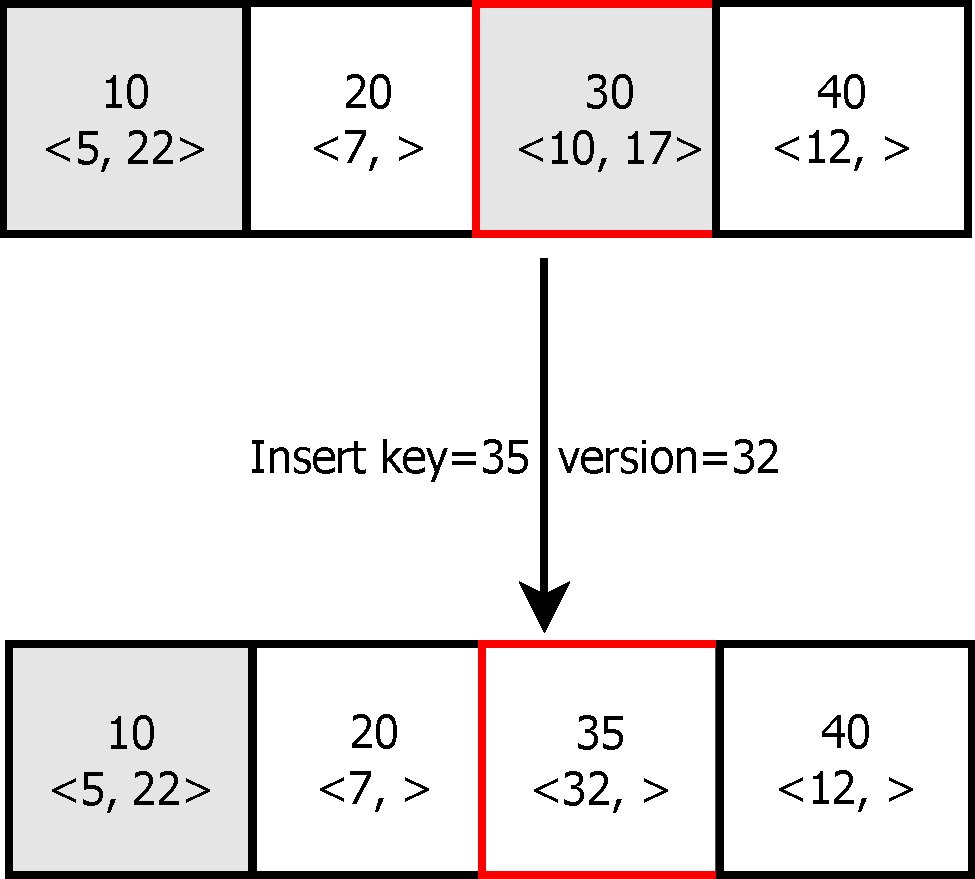
\includegraphics[width=\columnwidth]{figs/version_stealing}
%  \caption{Example of space reuse in a B-Tree leaf}
%  \label{fig:reuse-ver} 
%\end{figure}

If no free or dead entry was found, a \texttt{split\_insert}, similar
to a traditional B-Tree split, would be performed. \texttt{split\_insert},
shown in Algorithm~\ref{alg:btree_split_insert}, is a copy-on-write style
operation in which existing entries are copied before making a
modification. As an example, consider the node shown in 
Figure~\ref{fig:split_example}, where the key $40$ is being inserted.  
We only need to preserve the `live' entries for further updates and 
\texttt{split\_insert} creates one or two new nodes based on the number
of live entries present. Note that setting the end version
(lines~\ref{line:i_endversion}--\ref{line:i_endversion_end}) is the
only change made to the existing leaf node. This ensures that older
data versions are not affected by failures. In this case, two new
nodes are created at the end of the split.

We perform two operations to update the inner nodes after such a split.
First, the entry corresponding to the now-dead child node is marked
as dead. Next, new entries are inserted with links pointing to the
newly created leaf nodes. If the inner node overflows during this process
a \texttt{split\_insert} is performed to create new inner nodes.
When the root node of a tree overflows, we split the root node and
create one or two new nodes. We then create a new root node with links
to the old root and to the newly created split-nodes. The pointer to
the root node is updated atomically to ensure safety. 

% This is related to the problem with the right most key/pointer.
% The 'key' to be inserted for a new node is
%   -max key of the child node unless
%   -we are marking the largest key as dead. in this case use old key
%    for the larger of the two child nodes. 

\begin{figure}[t]
\vspace{0.15in}
\begin{center}
\begin{tikzpicture}[scale=0.75, transform shape]
 \begin{scope}[xshift=2.5cm]
   \node[nd={l,l,l}] (a1) {
    \btnode{text}{5}{2}{-}
    \btnode{second}{20}{3}{-}
    \btnode{third}{99}{1}{-}
 };
   \node[nd={l,l,l}, rectangle split ignore empty parts=true] (a2) [right=of a1] {
    \btnode{text}{40}{4}{-}
 };
 \end{scope}

 \begin{scope}[yshift=-1.75cm,
   every node/.style=draw,node distance=2mm]
   \node[nd={d,d,d}] (b1) {
    \btnode{text}{5}{2}{4}
    \btnode{second}{20}{3}{4}
    \btnode{third}{99}{1}{4}
 };
   \node[nd={l,l,l},rectangle split ignore empty parts=true]  (b2) [right=of b1]{
    \btnode{text}{5}{4}{-}
    \btnode{second}{20}{4}{-}
 };
   \node[nd={l,l,l},rectangle split ignore empty parts=true]  (b3) [right=of b2]{
    \btnode{text}{40}{4}{-}
    \btnode{second}{99}{4}{-}
 };
   \draw [very thick, dashed](-2,0.9) --(7,0.9) ;
 \end{scope}

\draw [->,very thick, densely dashed, -stealth] (a2) -- (a1) node[pos=0.5,above]{Insert};
\draw [->, densely dotted, thick, shorten >= 10pt, shorten <= 10pt] (a1.south) to (b1.north);
%\draw [->,very thick,dashed] (a1) to (b2);
%\draw [->,very thick,dashed] (a1) to (b3);
\end{tikzpicture}
\end{center}
%\vspace{-0.15in}
\caption{CDDS node split during insertion}
\label{fig:split_example}
%\vspace{-0.15in}
\end{figure}


%\begin{figure}[tbh]
%\begin{tikzpicture}
%\begin{scope}[xshift=2.5cm]
%\node[nd={l,l,l,l,l,l,l,l}, rectangle split parts=8] {
%   \btnode{text}{5}{1}{-}
%   \btnode{second}{10}{2}{-}
%   \btnode{third}{20}{3}{-}
%   \btnode{four}{30}{4}{6}
%   \btnode{five}{40}{5}{7}
%   \btnode{six}{50}{8}{-}
%   \btnode{seven}{60}{9}{-}
%   \btnode{eight}{70}{10}{-}
%};
%\end{scope}
%\end{tikzpicture}
% \caption{Occupancy}
% \label{fig:occ_example}
%\end{figure}

%To ensure durability, the \texttt{flush} command is used to push the
%new entry to persistent storage (line~\ref{line:i_nslot_flush}
%or~\ref{line:i_ny_flush}) before updating and \texttt{flush}ing the
%current consistent version
%(lines~\ref{line:i_upv}--\ref{line:i_flush_version}).  
Once all the changes have been \texttt{flush}ed to persistent storage,
the current consistent version is updated atomically
(lines~\ref{line:i_upv}--\ref{line:i_flush_version}).  At this point,
the update has been successfully committed to the NVBM and failures
will not result in the update being lost.

%New reader threads will also
%be able to access the updated version of the CDDS.

\subsection{Deletion}
\label{sec:btree_delete}

\begin{algorithm}[t]
\dontprintsemicolon
\linesnumbered

\SetAlFnt{\sf}
\SetAlCapFnt{\sf}

\SetKwFunction{GetCurrentConsistentVersion}{get\_current\_consistent\_version}
\SetKwFunction{GetNumEntries}{get\_num\_entries}
\SetKwFunction{SetNumEntries}{set\_num\_entries}
\SetKwFunction{CanReuseVersion}{can\_reuse\_version}
\SetKwFunction{MergeWithSibling}{merge\_with\_sibling}
\SetKwFunction{Flush}{flush}
\SetKwFunction{NumLiveEntries}{num\_live\_entries}
\SetKwFunction{Insert}{insert}
\SetKwFunction{NewNode}{new\_node}
\SetKwFunction{Delete}{delete}
\SetKwFunction{FindEntry}{find\_entry}
\SetKwFunction{PickSibling}{pick\_sibling}
\SetKwFunction{CopyFromSibling}{copy\_from\_sibling}

\KwIn{k: key, r: root}
\Begin(\Delete{k, r}) {
  $v \leftarrow current\_version$\;
  $v'\leftarrow v+1$\; 
  \tcp{Recurse to leaf node (n)}\;
  %\vdots\;
  %\BlankLine
  $y \leftarrow \FindEntry{n, k} $\;
  $n[y].end \leftarrow v' $\;
  $l \leftarrow \NumLiveEntries{n} $\;
  \If(\tcp*[f]{Underflow}){$l = m_{l}$} {  \nllabel{line:i_underflow}
    $s \leftarrow \PickSibling{n} $\;
    $l_{s} \leftarrow \NumLiveEntries{s} $\;
    \If { $l_{s} > 3\times m_{l}$ } {
      %\tcp{Copy $m_{l}$ keys from sibling} \;
      \CopyFromSibling{$n$, $s$, $v'$} \;
    }
    \lElse {
      \MergeWithSibling{$n$, $s$, $v'$}\;
    }
    \tcp{Update inner nodes}\;
  } \lElse {
    \Flush{$n[y]$} \; 
  }
  %\BlankLine
  %\vdots\;
  %\BlankLine
  $current\_version \leftarrow v'$\; 
  \Flush{$current\_version$}\;      
}

\BlankLine
\KwIn{n: node, s: sibling, v:version}
\Begin(\MergeWithSibling{n, s, v}){
    $y \leftarrow \GetNumEntries{s} $\;
    \If {$y < 4 \times m_{l}$}{
%      \tcp{Insert $m_{l}$ keys in sibling}
      \For {$i = 1$ to $m_{l}$} { 
        \Insert{$s, n[i].key, v$}\;
        $n[i].end \leftarrow v$\;
      }
    }
    \Else {
%      \tcp{Create new node}
      $nn \leftarrow \NewNode $\;
      $l_{s} \leftarrow \NumLiveEntries{s} $\;
      \For {$i = 1$ to $l_{s}$} { 
        \Insert{$nn, s[i].key, v$}\;
        $s[i].end \leftarrow v$\;
      }
      \For {$i = 1$ to $m_{l}$} { 
        \Insert{$nn, n[i].key, v$}\;
        $n[i].end \leftarrow v$\;
      }
      \Flush{$nn$} \;
    }
    \Flush{$n, s$} \;
}


\BlankLine
\KwIn{n: node, s: sibling, v: version}
\Begin(\CopyFromSibling{n, s, v}){
%    \tcp{Omitted for brevity}
%    \tcp{Create new node}
    $nn \leftarrow \NewNode $\;
    \For {$i = 1$ to $m_{l}$} { 
      \Insert{$nn, s[i].key$}\;
      $s[i].end \leftarrow v$\;
      \Insert{$nn, n[i].key$}\;
      $n[i].end \leftarrow v$\;
    }
    \Flush{$nn, n, s$} \;
}

\caption{CDDS B-Tree Deletion}
\label{alg:btree_delete}
\end{algorithm}



Deleting an entry is conceptually simple as it simply involves setting
the end version number for the given key.  It does not require
deleting any data as that is handled by GC\@.  However, in order to
bound the number of live blocks in the B-Tree and improve space
utilization, we shift live entries if the number of live entries per
node reaches $m_{l}$, a threshold defined in
Chapter~\ref{sec:space_analysis}.  The only exception is the root node
as, due to a lack of siblings, shifting within the same level is not
feasible.  However, as described in Chapter~\ref{sec:gc}, if the root
only contains one live entry, the child will be promoted.

As shown in Algorithm~\ref{alg:btree_delete}, we first check if the
sibling has at least $3\times m_{l}$ live entries and, if so, we copy
$m_{l}$ live entries from the sibling to form a new node. As the leaf
has $m_{l}$ live entries, the new node will have $2\times m_{l}$ live
entries. If that is not the case, we check if the sibling has enough
space to copy the live entries. Otherwise, as shown in
Figure~\ref{fig:merge_example}, we merge the two nodes to create a new
node containing the live entries from the leaf and sibling
nodes. The number of live entries in the new node will be $\geq 2
\times m_{l}$. The copy and merge operations only update the end
versions of existing entries and do not affect their contents.
The inner nodes are updated by marking end versions for the now-dead leaf
nodes and adding pointers to any newly created nodes. Since new nodes
are inserted in this operation, the inner nodes could overflow and
we use functions described in Chapter~\ref{sec:btree_insert} to
handle this.  After all the changes have been flushed to persistent
memory, the current consistent version is incremented.


\subsection{Garbage Collection}
\label{sec:gc}

As shown in Chapter~\ref{sec:btree_delete}, the size of the B-Tree
does not decrease when keys are deleted and can increase due to the
creation of new nodes.  To reduce the space overhead, we therefore use
a periodic GC procedure. It should be noted that while we use 
versioning as technique for performing consistent updates, we do
not need to retain obsolete versions. 

The GC procedure needs to take into account the fact that a B-Tree node
can have more than one parent. This can happen during the
 \texttt{split\_insert} operation and an example can be seen in
Figure~\ref{fig:cd-btree}. For this reason, we divide the GC procedure
into two parts. The first is a \textit{logical} procedure which removes
pointers that will no longer be used and the second, a \textit{physical}
procedure where dead nodes are deleted and allocated memory is
reclaimed.  The former procedure is described in
Algorithm~\ref{alg:btree_gc} and starts from the root of the B-Tree.
If an inner node entry has died before the current consistent version,
the pointer from the inner node to the child node can be removed.
This is because the pointer is only used to lookup elements older than
the current consistent version and will not be used by future operations.
Any live entries are preserved and entries are left-shifted to overwrite
removed entries. This procedure is recursively repeated till we reach the leaf
nodes.  If a node contains only one live entry after garbage collection, 
the child pointed to by the entry is promoted.  This helps reduce the height
of the B-Tree.  As seen in the transformation of Figure~\ref{fig:cd-btree} to
the reduced-height tree shown in Figure~\ref{fig:cd-btree-gc}, only live
nodes are present after GC\@.  \textit{Physical} GC is currently implemented
using a mark-and-sweep garbage collector~\citep{Boehm98}.  While a reference
counting implementation might also suffice, it would entail the overhead of
flushing reference counts.

% Run periodically based on two conditions: every 'n' versions or after
% some time period.

\begin{algorithm}[t]
\dontprintsemicolon
\linesnumbered

\SetAlFnt{\sf}
\SetAlCapFnt{\sf}

\SetKwFunction{GetLastConsistentVersion}{get\_last\_consistent\_version}
\SetKwFunction{GetNumEntries}{get\_num\_entries}
\SetKwFunction{SetNumEntries}{set\_num\_entries}
\SetKwFunction{NumLiveEntries}{num\_live\_entries}
\SetKwFunction{IsInnerNode}{is\_inner\_node}
\SetKwFunction{GarbageCollect}{garbage\_collect}

\KwIn{n: node}
\Begin(\GarbageCollect{n}){
    \If { \IsInnerNode{n} } {
      $v \leftarrow \GetLastConsistentVersion$\; 
      $shift \leftarrow 0$\;
      $y \leftarrow \GetNumEntries{n}$\;
      \For {$i = 1$ to $y$} {
          \If {$n[i].end \neq 0$ and $n[i].end < v$} {
              $n[i].child = null$\;
              $shift++$\;
          }
          \Else {
              \GarbageCollect{$n[i].child$}\;
              \If { $shift \neq 0$ } {
                $n[i - shift].child = n[i].child$\; 
                $n[i - shift].key = n[i].key$\;
                $n[i - shift].start = n[i].start$\;
                $n[i - shift].end = n[i].end$\;
              }
          }
      }
      \SetNumEntries{$n$, $y - shift$}\;
      \If { \GetNumEntries{$n$} = 1 } {
        \tcp{Use only child instead}
      }
    }
}
\caption{CDDS B-Tree Garbage Collection}
\label{alg:btree_gc}
\end{algorithm}


%Based on the memory available, we can also remove dead entries in the
%remaining live nodes. However this would entail locking the tree and
%affect the throughput of the normal B-Tree operations. Also
%traditional garbage collection schemes can be integrated with the
%garbage collection algorithm.

\begin{figure}[t]
\begin{minipage}[c]{0.48\textwidth}
\begin{tikzpicture}[scale=0.75, transform shape]
\vspace{0.15in}
 \begin{scope}[xshift=2.5cm]
   \node[nd={l,l,d}] (a1) {
    \btnode{text}{5}{4}{-}
    \btnode{second}{10}{5}{-}
    \btnode{third}{20}{4}{8}
 };
   \node[nd={d,l,l}] (a2) [right=of a1] {
    \btnode{text}{30}{7}{9}
    \btnode{second}{40}{4}{-}
    \btnode{third}{99}{4}{-}
 };
\draw [<->, very thick, densely dashed, stealth-stealth] (a2) -- (a1) node[pos=0.5,above]{Merge};
 \end{scope}

 \begin{scope}[yshift=-1.75cm,
   every node/.style=draw,node distance=2mm]
   \node[nd={d,d,d}] (b1) {
    \btnode{text}{5}{4}{10}
    \btnode{second}{10}{5}{10}
    \btnode{third}{20}{4}{8}
 };
   \node[nd={d,d,d}]  (b2) [right=of b1]{
    \btnode{text}{30}{7}{9}
    \btnode{second}{40}{4}{10}
    \btnode{third}{99}{4}{10}
 };
 \node[nd={l,l,l}]  (b3) [right=of b2]{
    \btnode{text}{5}{10}{-}
    \btnode{second}{40}{10}{-}
    \btnode{third}{99}{10}{-}
 };
 \draw [very thick, dashed](-1.75,0.9) --(9,0.9);
 \end{scope}

 %\draw [->,very thick,dashed,bend left=10] (before) to (b2);
\draw [->, densely dotted, thick, shorten >= 10pt, shorten <= 10pt] (a1.south) to (b1.north);
\draw [->, densely dotted, thick, shorten >= 10pt, shorten <= 10pt] (a2.south) to (b2.north);
\end{tikzpicture}
\caption{CDDS node merge during deletion}
\label{fig:merge_example}
\end{minipage}
\begin{minipage}[c]{0.48\textwidth}
\centerline{
\begin{tikzpicture}[scale=0.75, transform shape]
\begin{scope}
[level 1/.style={sibling distance=3cm}]
[node distance=2cm on grid, >=stealth', auto, inner sep=0mm]
 \node[nd={l,l,l}] {
    \btnode{text}{10}{6}{-}
    \btnode{second}{20}{6}{-}
    \btnode{third}{99}{6}{-}
 }
 child {node[nd={l,l,l}] {
     \btnode{text}{5}{6}{-}
     \btnode{second}{8}{7}{-}
     \btnode{third}{10}{6}{-}
   }
 }
 child {node[nd={l,d,l}] {
     \btnode{text}{13}{9}{-}
     \btnode{second}{15}{6}{8}
     \btnode{third}{20}{6}{-}
   }
 }
 child{node[nd={l,l,l}] (c3) {
     \btnode{text}{40}{4}{-}
     \btnode{second}{99}{4}{-}
     }
 };
\end{scope}
\end{tikzpicture}
}
\caption{CDDS B-Tree after Garbage Collection}
\label{fig:cd-btree-gc}
\end{minipage}
\end{figure}

\begin{figure}[t]
\begin{minipage}[c]{0.48\textwidth}
\centerline{
\begin{tikzpicture}[scale=0.75, transform shape]
\begin{scope}
[level 1/.style={sibling distance=3.1cm}]
[node distance=2cm on grid, >=stealth', auto, inner sep=0mm]
 \node[nd={d,d,d}] {
    \btnode{text}{20}{4}{6}
    \btnode{second}{99}{1}{4}
    \btnode{third}{99}{4}{6}
 }
 child {node[nd={d,d,d}] {
     \btnode{text}{5}{4}{6}
     \btnode{second}{10}{5}{6}
     \btnode{third}{20}{4}{6}
   }
 }
 child {node[nd={d,d,d}] {
     \btnode{text}{5}{2}{4}
     \btnode{second}{20}{3}{4}
     \btnode{third}{99}{1}{4}
   }
 }
 child{node[nd={l,l,l}] (c3) {
     \btnode{text}{40}{4}{-}
     \btnode{second}{99}{4}{-}
     }
 };
\end{scope}
\begin{scope}
\node (live) [font=\large, yshift=1cm, rectangle,draw=black!0] {Current Consistent Version - 5};
\end{scope}
\end{tikzpicture}
}
\caption{CDDS B-Tree before Recovery}
\label{fig:cd-btree-pre-recovery}
\end{minipage}
\begin{minipage}[c]{0.48\textwidth}
\centerline{
\begin{tikzpicture}[scale=0.75, transform shape]
\begin{scope}
[level 1/.style={sibling distance=3.1cm}]
[node distance=2cm on grid, >=stealth', auto, inner sep=0mm]
 \node[nd={l,d,l}] {
    \btnode{text}{20}{4}{-}
    \btnode{second}{99}{1}{4}
    \btnode{third}{99}{4}{-}
 }
 child {node[nd={l,l,l}] {
     \btnode{text}{5}{4}{-}
     \btnode{second}{10}{5}{-}
     \btnode{third}{20}{4}{-}
   }
 }
 child {node[nd={d,d,d}] {
     \btnode{text}{5}{2}{4}
     \btnode{second}{20}{3}{4}
     \btnode{third}{99}{1}{4}
   }
 }
 child{node[nd={l,l,l}] (c3) {
     \btnode{text}{40}{4}{-}
     \btnode{second}{99}{4}{-}
     }
 };
\end{scope}
\end{tikzpicture}
}
\caption{CDDS B-Tree after Recovery}
\label{fig:cd-btree-post-recovery}
\end{minipage}
\end{figure}

\begin{algorithm}[t]
\dontprintsemicolon
\linesnumbered

\SetAlFnt{\sf}
\SetAlCapFnt{\sf}

\SetKwFunction{GetLastConsistentVersion}{get\_last\_consistent\_version}
\SetKwFunction{GetNumEntries}{get\_num\_entries}
\SetKwFunction{SetNumEntries}{set\_num\_entries}
\SetKwFunction{NumLiveEntries}{num\_live\_entries}
\SetKwFunction{IsInnerNode}{is\_inner\_node}
\SetKwFunction{RecoverNode}{recover\_node}

\KwIn{n: node}
\Begin(\RecoverNode{n}){
    $v \leftarrow \GetLastConsistentVersion$\; 
    $shift \leftarrow 0$\;
    $y \leftarrow \GetNumEntries{n}$\;
    \For {$i = 1$ to $y$} {
        \If {$n[i].start > v$} {
            \tcp{Created during}
            \tcp{partial operation}
            $shift++$\;
        }
        \Else {
            \If {$n[i].end > v$} {
                \tcp{Deleted during}
                \tcp{partial operation}
                $n[i].end = 0$\; 
            }
            \If { \IsInnerNode{n} } {
                \RecoverNode{$n[i].child$}\;
            }
            \If { $shift \neq 0$ } {
              $n[i - shift].key = n[i].key$\;
              $n[i - shift].start = n[i].start$\;
              $n[i - shift].end = n[i].end$\;
            }
        }
    }
    \SetNumEntries{$n$, $y - shift$}\;
}
\caption{CDDS B-Tree Recovery}
\label{alg:btree_recovery}
\end{algorithm}


\subsection{Failure Recovery}

The recovery procedure for the B-Tree is similar to garbage
collection.  In Algorithm~\ref{alg:btree_recovery}, we describe 
the logical phase in which we remove entries newer than 
the current consistent version. If an inner node entry was created
after the current consistent version, the pointer to the child node
can be removed as the update was interrupted before completion.  Also,
if an entry was deleted after the current consistent version, then the
entry is marked as live.  This procedure is repeated recursively
till we reach the leaf nodes.  Additionally, if there was a failure
while inserting in a sorted order, we could have duplicate entries 
in a node. We remove duplicate entries by shifting entries to the 
left and use the \texttt{flush} operation to ensure we don't introduce
any inconsistencies during recovery.

For example, consider the CDDS B-Tree shown in 
Figure~\ref{fig:cd-btree-pre-recovery}. The update operation which
inserts version $6$ has been interrupted due to a failure. The end
versions for nodes are marked as $6$, but newly created nodes have not
been linked to the B-Tree before the failure. Also, the current 
consistent version for the B-Tree is known to be $5$. In this case,
the recovery function changes the entries which ended at version $6$
to be live as shown in Figure~\ref{fig:cd-btree-post-recovery}.
Hence, the recovery function performs a physical `undo' of partial 
updates and ensures that the tree is physically and logically 
identical to the most recent consistent version.  While our current 
recovery implementation scans the entire data structure, the recovery
process is fast as it operates at memory bandwidth speeds and only 
needs to verify CDDS metadata.  While we believe that the recovery 
procedure is re-entrant, we are working towards verifying it using 
empirical evidence from fault injection tests. We are also exploring
formal verification techniques that can be used to verify the 
recovery protocol used in the CDDS B-Tree. 


\subsection{Space Analysis}
\label{sec:space_analysis}

In the CDDS B-Tree, space utilization can be characterized by the
number of live blocks required to store $N$ key-value pairs. Since the
values are only stored in the leaf nodes, we analyze the maximum
number of live leaf nodes present in the tree. In the CDDS B-Tree, a
new node is created by an insert or delete operation.  As
described in Chapters~\ref{sec:btree_insert}
and~\ref{sec:btree_delete}, the minimum number of live entries in
new nodes is $2\times m_{l}$.

When the number of live entries in a node reaches $m_{l}$, it is
either merged with a sibling node or its live entries are copied to a
new node.  Hence, the number of live entries in a node is $>m_{l}$.
Therefore, in a B-Tree with $N$ live keys, the maximum number of live
leaf nodes is bound by $O(\frac{N}{m_{l}})$. Choosing $m_{l}$ as
$\frac{k}{5}$, where $k$ is the size of a B-Tree node, the maximum
number of live leaf nodes is $O(\frac{5N}{k})$.

For each live leaf node, there is a corresponding entry in the parent
node.  Since the number of live entries in an inner node is also
$>m_{l}$, the number of parent nodes required is
$O\left(\frac{\frac{5N}{k}}{m_{l}}\right) =
O(\frac{N}{(\frac{k}{5})^2})$. Extending this, we can see that the
height of the CDDS B-Tree is bound by $O(log_{\frac{k}{5}}N)$.  This
also bounds the time for all B-Tree operations.

\section{CDDS Discussion}
\label{sec:cdds_discuss}

Apart from the CDDS B-Tree operations described above, the
implementation also supports additional features including iterators
and range scans.  We believe that CDDS versioning also lends itself to
other powerful features such as instant snapshots, rollback for
programmer recovery, and integrated NVBM wear-leveling.  We hope to
explore these issues in our future work. 

One of the limitations of our CDDS-BTree implementation is that we have
an equal number of pointers and keys in an inner node.  This is different
from a traditional B-Tree which has an extra pointer for keys larger
than those stored in the node. This is an implementation artifact that 
makes it easier to track the start and end versions of a pointer.  
As a consequence, the key with maximum value needs to be first inserted 
to avoid any imbalance while inserting other keys.  In practice this is 
overcome easily by having a maximum key which the comparator function 
recognizes and this imposes limited overhead in the implementation.  

We also do not anticipate the design of a CDDS preventing the
implementation of different concurrency schemes.  Our current CDDS
B-Tree implementation uses a multiple-reader, single-writer model.
However, the use of versioning lends itself to more complex
concurrency control schemes including multi-version concurrency
control (MVCC)~\citep{Bernstein81}.  While beyond the scope of this
paper, exploring different concurrency control schemes for CDDSs is a
part of our future work.

Finally, apart from multi-version data
structures~\citep{Becker96,Varman97}, CDDSs have also been influenced
by Persistent Data Structures (PDSs)~\citep{Driscoll89}.  The
``Persistent'' in PDS does not actually denote durability on
persistent storage but, instead, represents immutable data structures
where an update always yields a new data structure copy and never
modifies previous versions.  The CDDS B-Tree presented above is a
weakened form of semi-persistent data structures.  We modify previous
versions of the data structure for efficiency but are guaranteed to
recover from failure and rollback to a consistent state.  However, the
PDS concepts are applicable, in theory, to all linked data structures.
%% and, in theory, also for flat memory objects~\citep{Dietz89}.
Using PDS-style techniques, we have implemented a proof-of-concept
CDDS hash table and, as evidenced by previous work for functional
programming languages~\citep{Okasaki99}, we are confident that CDDS
versioning techniques can be extended to a wide range of data
structures.

\section{Tembo: A CDDS Key-Value Store}
\label{sec:kv}

We created Tembo, a CDDS Key-Value (KV) store, to evaluate the
effectiveness of a CDDS-based data store.  The system involves the
integration of the CDDS-based B-Tree described in
Chapter~\ref{sec:cdds_btree} into Redis~\citep{Redis}, a widely used
event-driven KV store.  As our contribution is not based around the
design of this KV system, we only briefly describe Tembo in this
section.  As shown in Chapter~\ref{sec:impl_effort}, the integration
effort was minor and leads us to believe that retrofitting CDDS into
existing applications will be straightforward.


The base architecture of Redis is well suited for a CDDS as it retains
the entire data set in RAM\@.  This also allows an unmodified Redis to
serve as an appropriate performance baseline.  While persistence in
the original system was provided by a write-ahead append-only log,
this is eliminated in Tembo because of the CDDS B-Tree integration.
For fault-tolerance, Tembo provides master-slave replication with
support for hierarchical replication trees where a slave can act as
the master for other replicas.  Consistent hashing~\citep{Karger97} is
used by client libraries to distribute data in a Tembo cluster.


% Finally, given that the above two instructions have been support by
% Intel and AMD since 2000 and 2003 respectively, we believe that
% assuming their existence for NVBM-based machines is safe.  We can
% also use the \texttt{cpuid} feature (\texttt{/proc/cpuinfo} on Linux
% contains this information) to verify their presence at program
% startup.


% LocalWords:  CDDSs CDDS Versioning multi versioning multiversion API nd num
% LocalWords:  GetCurrentConsistentVersion GetNumEntries SetNumEntries GC nslot
% LocalWords:  InsertKey NumLiveEntries NewNode Recurse upv endversion sep ny
% LocalWords:  FindEntry PickSibling CopyFromSibling xshift SplitInsert nn pos
% LocalWords:  GetLastConsistentVersion CanReuseVersion lookup clflush mfence
% LocalWords:  MergeWithSibling MarkAsEnd metadata NVBM wbinvd AMD cacheline ns
% LocalWords:  microbenchmarks Varman Boehm DMA recurse MVCC DMAs pseudocode
% LocalWords:  IOMMUs PDSs PDS PCI syscall POSIX NVBM's userspace APIs roadmaps
% LocalWords:  mmap RVM Tembo ing rebalancing
% LocalWords:  CDDS Redis KV Tembo

\begin{comment}
\section{Tembo: A CDDS Key-Value Store}
\label{sec:kv}

We created Tembo, a CDDS Key-Value (KV) store, to evaluate the
effectiveness of a CDDS-based data store.  The system involves the
integration of the CDDS-based B-Tree described in
Chapter~\ref{sec:cdds_btree} into Redis~\citep{Redis}, a widely used
event-driven KV store.  As our contribution is not based around the
design of this KV system, we only briefly describe Tembo in this
section.  As shown in Chapter~\ref{sec:impl_effort}, the integration
effort was minor and leads us to believe that retrofitting CDDS into
existing applications will be straightforward.


The base architecture of Redis is well suited for a CDDS as it retains
the entire data set in RAM\@.  This also allows an unmodified Redis to
serve as an appropriate performance baseline.  While persistence in
the original system was provided by a write-ahead append-only log,
this is eliminated in Tembo because of the CDDS B-Tree integration.
For fault-tolerance, Tembo provides master-slave replication with
support for hierarchical replication trees where a slave can act as
the master for other replicas.  Consistent hashing~\citep{Karger97} is
used by client libraries to distribute data in a Tembo cluster.

% LocalWords:  CDDS Redis KV Tembo
\end{comment}

\chapter{Evaluation}
\label{sec:eval}

In this section, we evaluate our design choices in building Consistent
and Durable Data Structures.  First, we measure the overhead
associated with techniques used to achieve durability on existing
processors.  We then compare the CDDS B-tree to Berkeley DB and
against log-based schemes.  After briefly discussing CDDS
implementation and integration complexity, we present results from a
multi-node distributed experiment where we use the Yahoo Cloud Serving
Benchmark (YCSB)~\citep{Cooper10}.
% to compare Tembo to Cassandra~\citep{Lakshman10}.

\section{Evaluation Setup}

% HP Proliant DL360 G6

As NVBM is not commercially available yet, we used DRAM-based servers.
While others~\citep{Condit09} have shown that DRAM-based results are a good
predictor of NVBM performance, as a part of our ongoing work, we aim
to run micro-architectural simulations to confirm this within the
context of our work.  Our testbed consisted of 15 servers with two
Intel Xeon Quad-Core 2.67~GHz (X5550) processors and 48~GB RAM each.
The machines were connected via a full-bisection Gigabit Ethernet 
network.  Each processor has 128~KB L1, 256~KB L2, and 8~MB L3 caches.
While each server contained 8 300~GB 10K SAS drives, unless specified,
all experiments were run directly on RAM or on a ramdisk.  We
used the Ubuntu~10.04 Linux distribution and the 2.6.32-24 64-bit
kernel.

%  1333~MHz RAM. If you look at the processor specs, this becomes
%  clear.


\section{Flush Performance}
\label{sec:flush_perf}

\begin{figure}[t]
\begin{minipage}[b]{0.49\linewidth}
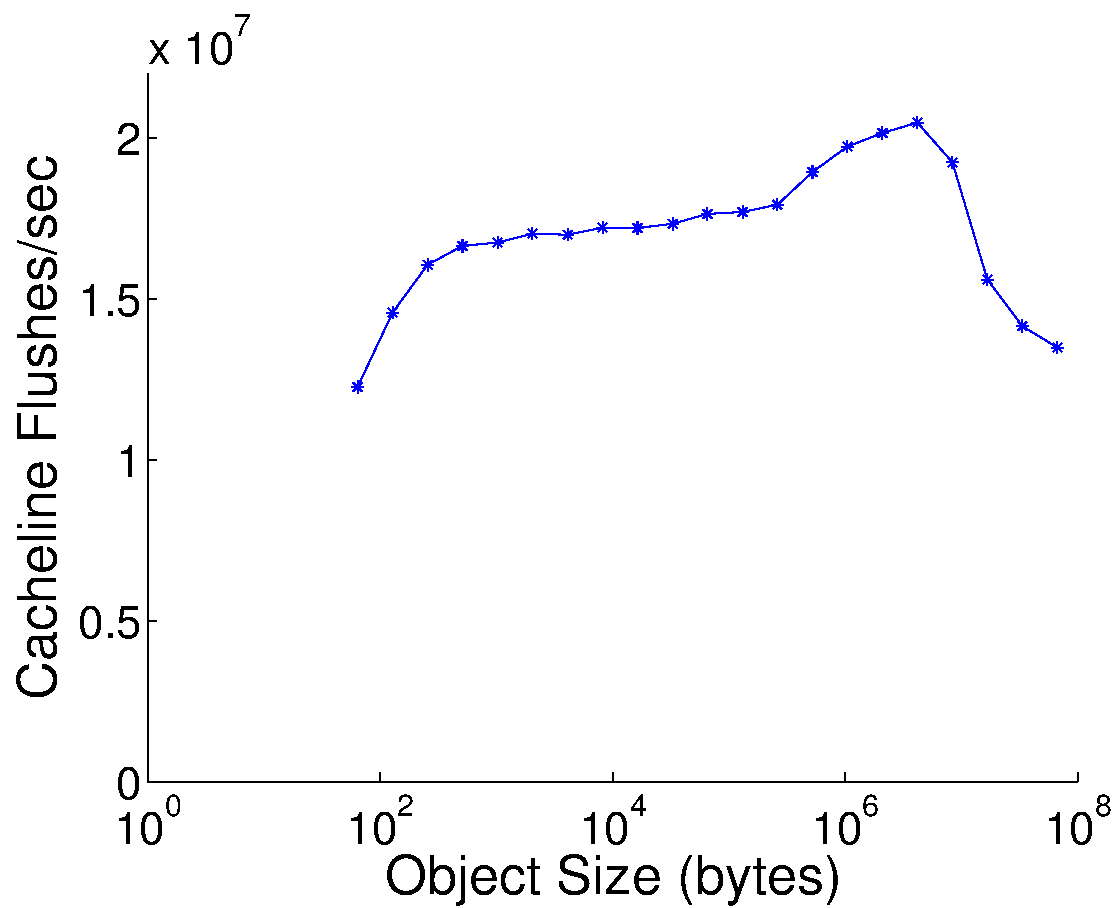
\includegraphics[width=\columnwidth]{figs/flushes_per_sec}
%\vspace{-0.3in}
\caption{Flushes/second}
\label{fig:flushes_per_sec}
\end{minipage}
%\hspace{0.1cm}
\begin{minipage}[b]{0.49\linewidth}
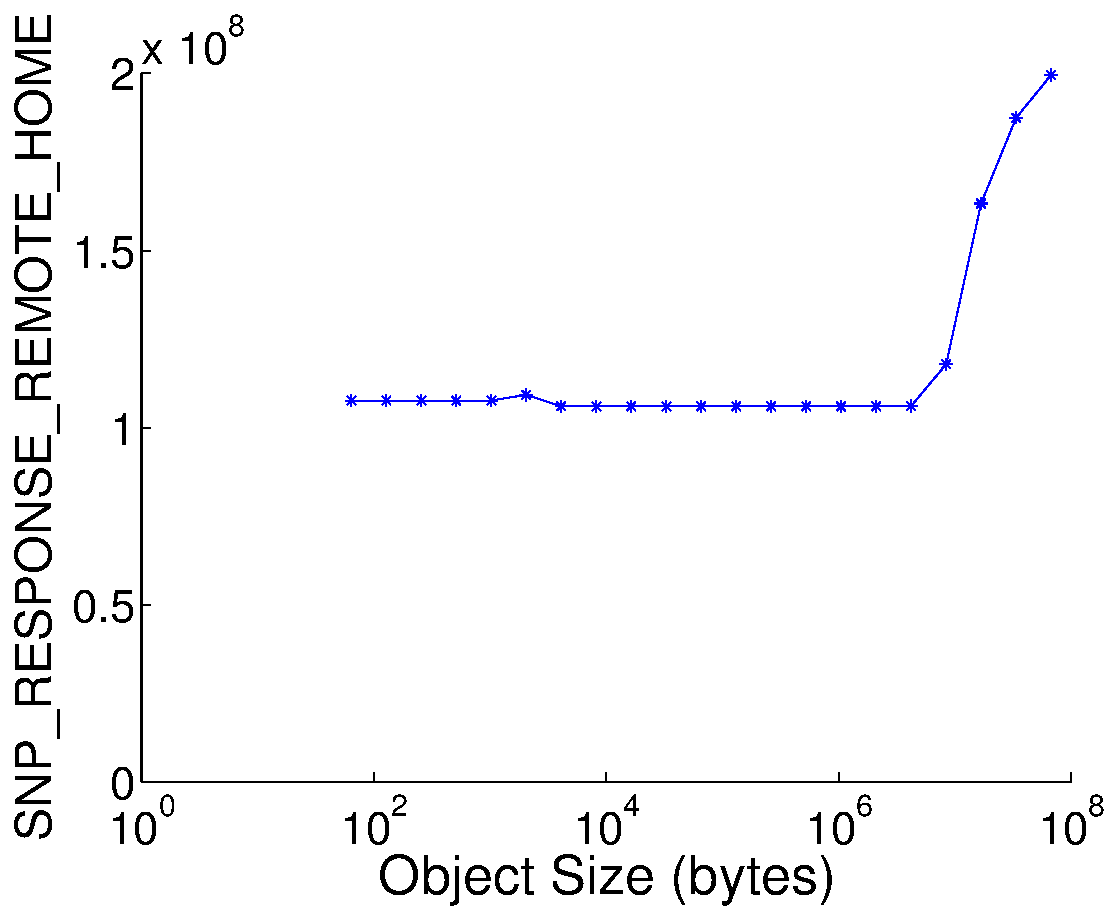
\includegraphics[width=\columnwidth]{figs/snoop_response}
%\vspace{-0.3in}
\caption{Cache Snooping}
\label{fig:ext_snoop}
\end{minipage}
%\vspace{-0.15in}
\end{figure}

To accurately capture the performance of the \texttt{flush} operation
defined in Chapter~\ref{sec:flush}, we used the ``MultCallFlushLRU''
methodology~\citep{Whaley08}.  The experiment allocates 64~MB of
memory and subdivides it into equally-sized cache-aligned objects.
Object sizes ranged from 64~bytes to 64~MB\@.  We write to every
cache line in an object, \texttt{flush} the entire object, and then
repeat the process with the next object.  For improved timing
accuracy, we stride over the memory region multiple times.

Remembering that each \texttt{flush} is a number of \texttt{clflush}es
bracketed by \texttt{mfence}s on both sides,
Figure~\ref{fig:flushes_per_sec} shows the number of
\texttt{clflush}es executed per second.  Flushing small objects sees
the worst performance ($\sim$12M cacheline flushes/sec for 64~byte
objects).  For larger objects (256~bytes--8~MB), the performance
ranges from $\sim$16M--20M cacheline flushes/sec.

\begin{sloppypar}
We also observed an unexpected drop in performance for large objects
($>$8~MB).  Our analysis showed that this was due to the cache
coherency protocol.  Large objects are likely to be evicted from the
L3 cache before they are explicitly flushed. A subsequent
\texttt{clflush} would miss in the local cache and cause a
high-latency ``snoop'' request that checks the second off-socket
processor for the given cache line.  As measured by the
UNC\_SNP\_RESP\_TO\_REMOTE\_HOME.I\_STATE performance counter, seen in
Figure~\ref{fig:ext_snoop}, the second socket shows a corresponding
spike in requests for cache lines that it does not contain.  To verify
this, we physically removed a processor and observed that the anomaly
disappeared\footnote{We did not have physical access to the
  experimental testbed and ran the processor removal experiment on a different
  dual-socket Intel Xeon (X5570) machine.}.  Further, as we could not
replicate this slowdown on AMD platforms, we believe that
cache-coherency protocol modifications can address this anomaly.
\end{sloppypar}

%These results show that \texttt{flush}'s performance is acceptable for
%most workloads because, unlike the artificial tight loop in this
%experiment, \texttt{flush}es are generally batched and only invoked
%when data needs to be made durable.

Overall, the results show that we can \texttt{flush} 0.72--1.19~GB/s
on current processors.  For applications without networking,
Chapter~\ref{sec:api_microbench} shows that future hardware support
can help but applications using \texttt{flush} can still outperform
applications that use file system \texttt{sync} calls.  Distributed
applications are more likely to encounter network bottlenecks before
\texttt{flush} becomes an overhead.
%  Alternatively, a smarter implementation could interleave the
%  \texttt{clflush} and \texttt{fence} for large objects.

\section{API Microbenchmarks}
\label{sec:api_microbench}

\begin{figure}[t]
\begin{minipage}[b]{0.49\textwidth}
\centerline{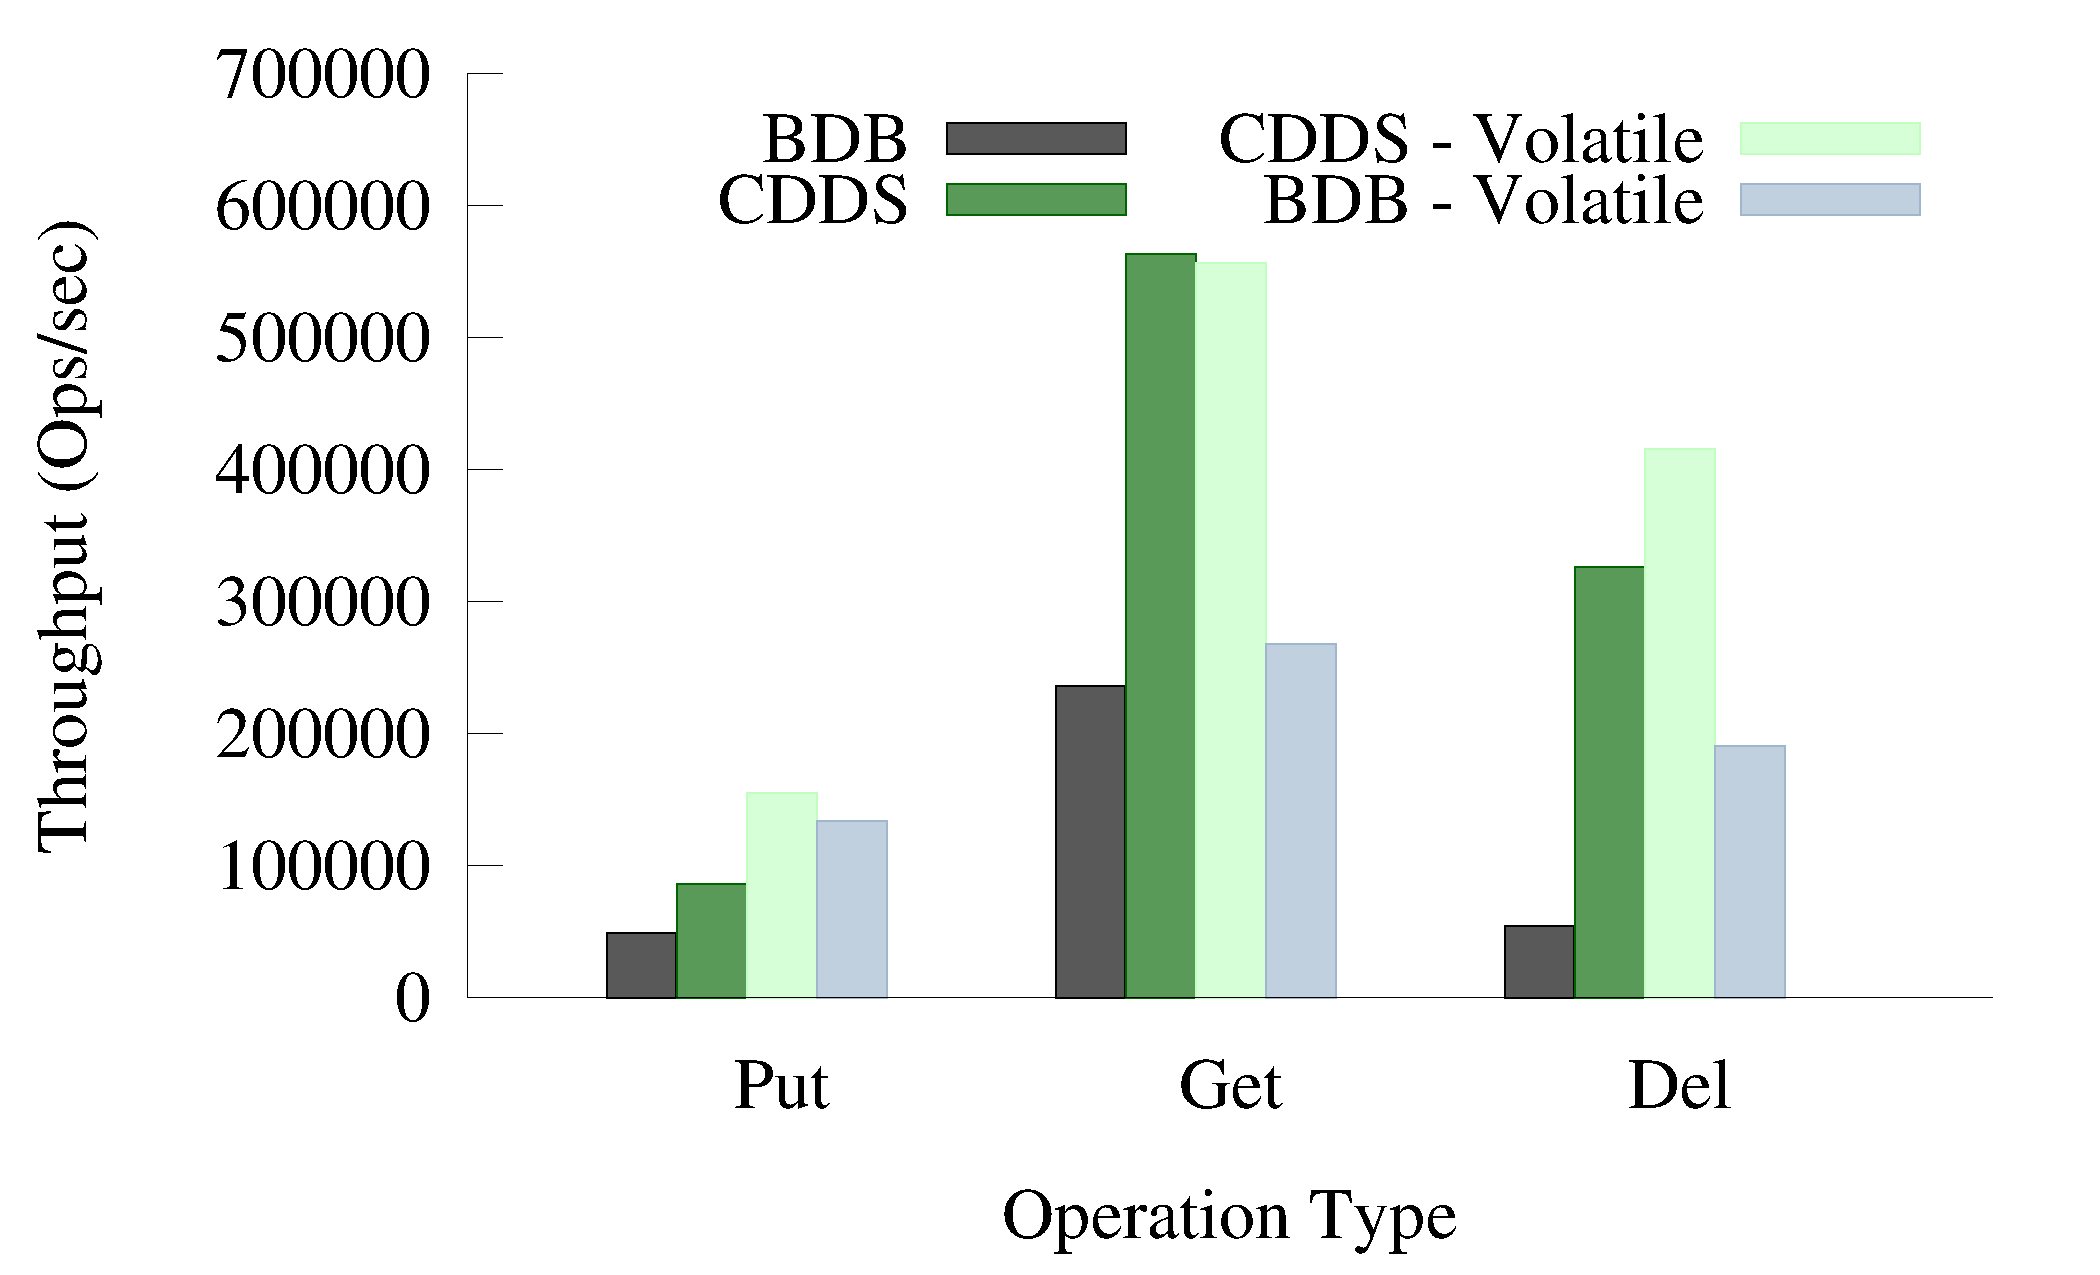
\includegraphics[width=\columnwidth]{figs/bdb-bench}}
\begin{captiontext}
\centerline{Mean of 5 trials. Max.\ standard deviation:
  2.2\% of the mean.}
\end{captiontext}
\caption{Berkeley DB Comparison}
\label{fig:bdb}
\end{minipage}
\begin{minipage}[b]{0.49\textwidth}
\centerline{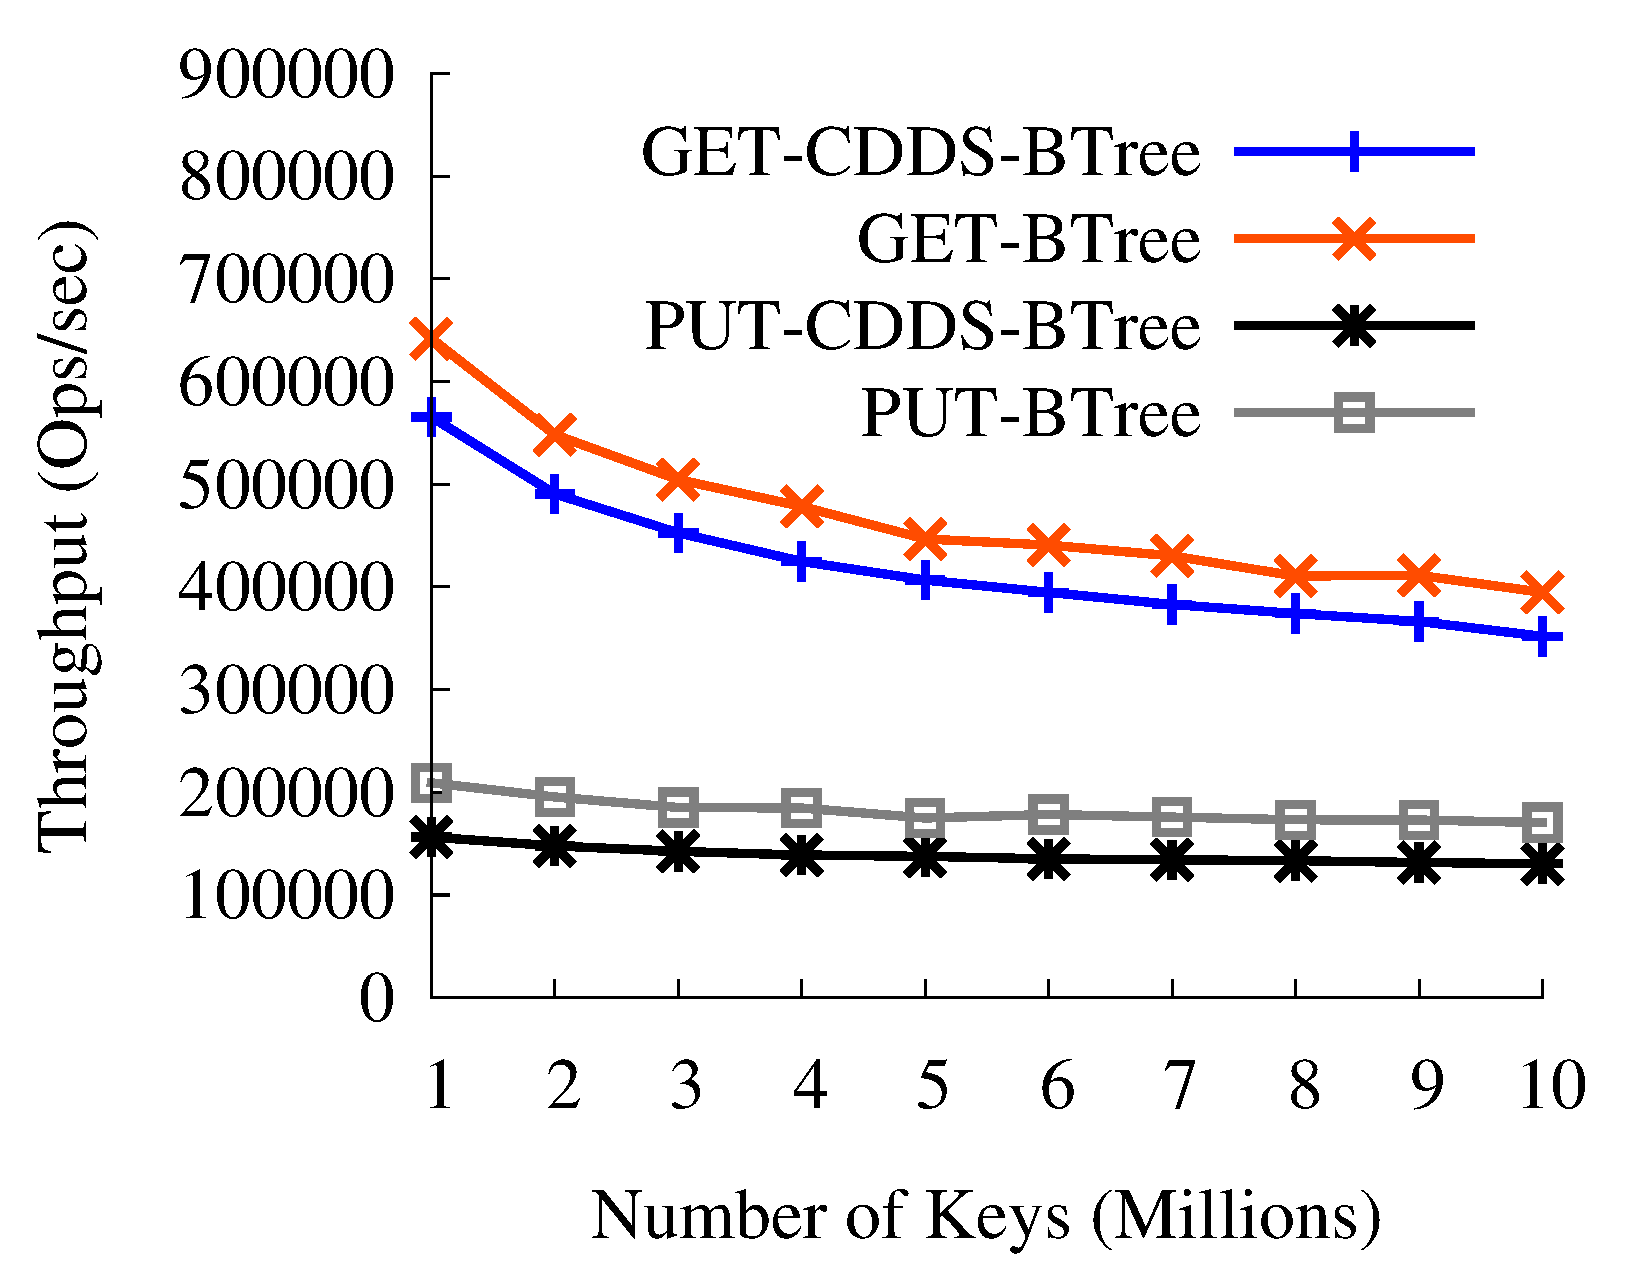
\includegraphics[width=0.85\columnwidth]{figs/versioning}}
%\begin{captiontext}
%\centerline{Mean of 5 trials. Max.\ standard deviation:
% 2.2\% of the mean.}
%\end{captiontext}
\caption{Versioning Overhead}
\label{fig:overhead}
\end{minipage}
\end{figure}

This section compares the CDDS B-Tree performance for puts, gets, and
deletes to Berkeley DB's (BDB) B-Tree implementation~\citep{Olson99}.
For this experiment, we insert, fetch, and then delete 1~million
key-value tuples into each system.  After each operation, we flush
the CPU cache to eliminate any variance due to cache contents.
Keys and values are 25 and 2048~bytes large.  The single-threaded
benchmark driver runs in the same address space as BDB and CDDS\@.
BDB's cache size was set to 8~GB and could hold the entire data
set in memory. Further, we configure BDB to maintain its log files
on an in-memory partition.

We run both CDDS and BDB (v4.8) in durable and volatile modes.  For
BDB volatile mode, we turn transactions and logging off.  For CDDS
volatile mode, we turn \texttt{flush}ing off.  Both systems in
volatile mode can lose or corrupt data and would not be used where
durability is required.  We only present the volatile results to
highlight predicted performance if hardware support was available and
to discuss CDDS design tradeoffs.

The results, displayed in Figure~\ref{fig:bdb}, show that, for
memory-backed BDB in durable mode, the CDDS B-Tree improves throughout
by 74\%, 138\%, and 503\% for puts, gets, and deletes respectively.
These gains come from not using a log (extra writes) or the file
system interface (system call overhead).  CDDS delete improvement is
larger than puts and gets because we do not delete data immediately
but simply mark it as dead and use GC to free unreferenced memory.  In
results not presented here, reducing the value size, and therefore the
log size, improves BDB performance but CDDS always performs better.

% XXX - Can we verify the 7\% improvement reason?

If zero-overhead epoch-based hardware support~\citep{Condit09} was
available, the CDDS volatile numbers show that performance of puts
and deletes would increase by 80\% and 27\% as \texttt{flush}es
would never be on the critical path. We do not observe any significant
change for gets as the only difference between the volatile and durable
CDDS is that the \texttt{flush} operations are converted into a noop.
%  We are still examining the reasons for the
% 6\% performance improvement in get operations but believe it to be a
% result of \texttt{flush} behavior.  As the puts immediately precede
% the gets, \texttt{flush}es in the durable case invalidate cache lines
% and they need to be brought back into cache for the next access.
% However, with the volatile CDDS, no \texttt{flush}es are used and the
% cache is warm for the get portion of the experiment.

% We see a large difference for delete performance because, as explained
% in Chapter~\ref{sec:btree_delete}, the durable CDDS B-Tree can create
% new nodes and invokes additional \texttt{flush}es.

We also notice that while volatile BDB throughput is lower than
durable CDDS for gets and dels by 52\% and 41\%, it is higher by 56\%
for puts.  Puts are slower for the CDDS B-Tree because of the work
required to maintain key ordering (described in
Chapter~\ref{sec:btree_lookup}), GC overhead, and a slightly higher
height due to nodes with a mixture of live and dead entries.  Volatile
BDB throughput is also higher than durable BDB but lower than volatile
CDDS for all operations.

To measure versioning overhead, we compared the volatile CDDS
B-Tree to a normal B-Tree~\citep{Bingman08}.  We performed the same
experiment described above and varied the input from one to
ten million keys. From the results, shown in Figure~\ref{fig:overhead},
we can see that the performance of the CDDS-BTree remains consistent
as we increase the number of keys. Also, we can see that volatile
CDDS's performance was lower than the in-memory B-Tree by 21\%-25\%
for puts and by 9\%-12\% for gets. This difference is similar to other
performance-optimized versioned B-trees~\citep{Soules03}.

% Put performance - BDB has no GC
% Get performance - BDB better because of smaller height tree

% 1. BDB Put is sensitive to value size. Decreasing value size reduces
% the performance difference.

% 2. CDDS (both) and B-tree (vanilla + not presented here) VERY
% sensitive to comparator.

% 3. Key size matters a lot for the delete. Reason is unverified but
% could be that CDDS does not erase value memory. GC does that.


\section{Implementation Effort}
\label{sec:impl_effort}



The CDDS B-Tree started with the STX C++ B-Tree~\citep{Bingman08}
implementation but, as measured by \texttt{sloccount} and shown in
Table~\ref{tab:integration}, the addition of versioning and NVBM
durability replaced 90\% of the code.  While the API remained the
same, the internal implementation differs substantially.  The
integration with Redis to create Tembo was simpler and only changed
1.7\% of code and took less than a day to integrate.  Since the CDDS
B-Tree implements an interface similar to an STL Sorted Container, we
believe that integration with other systems should also be simple.
Overall, our experiences show that while the initial implementation
complexity is moderately high, this only needs to be done once for a
given data structure.  The subsequent integration into legacy
or new systems is straightforward.


\section{Tembo Versioning vs.\ Redis Logging}
\label{sec:versioning_logging}

\begin{table}[t]
\begin{minipage}[b]{0.49\textwidth}
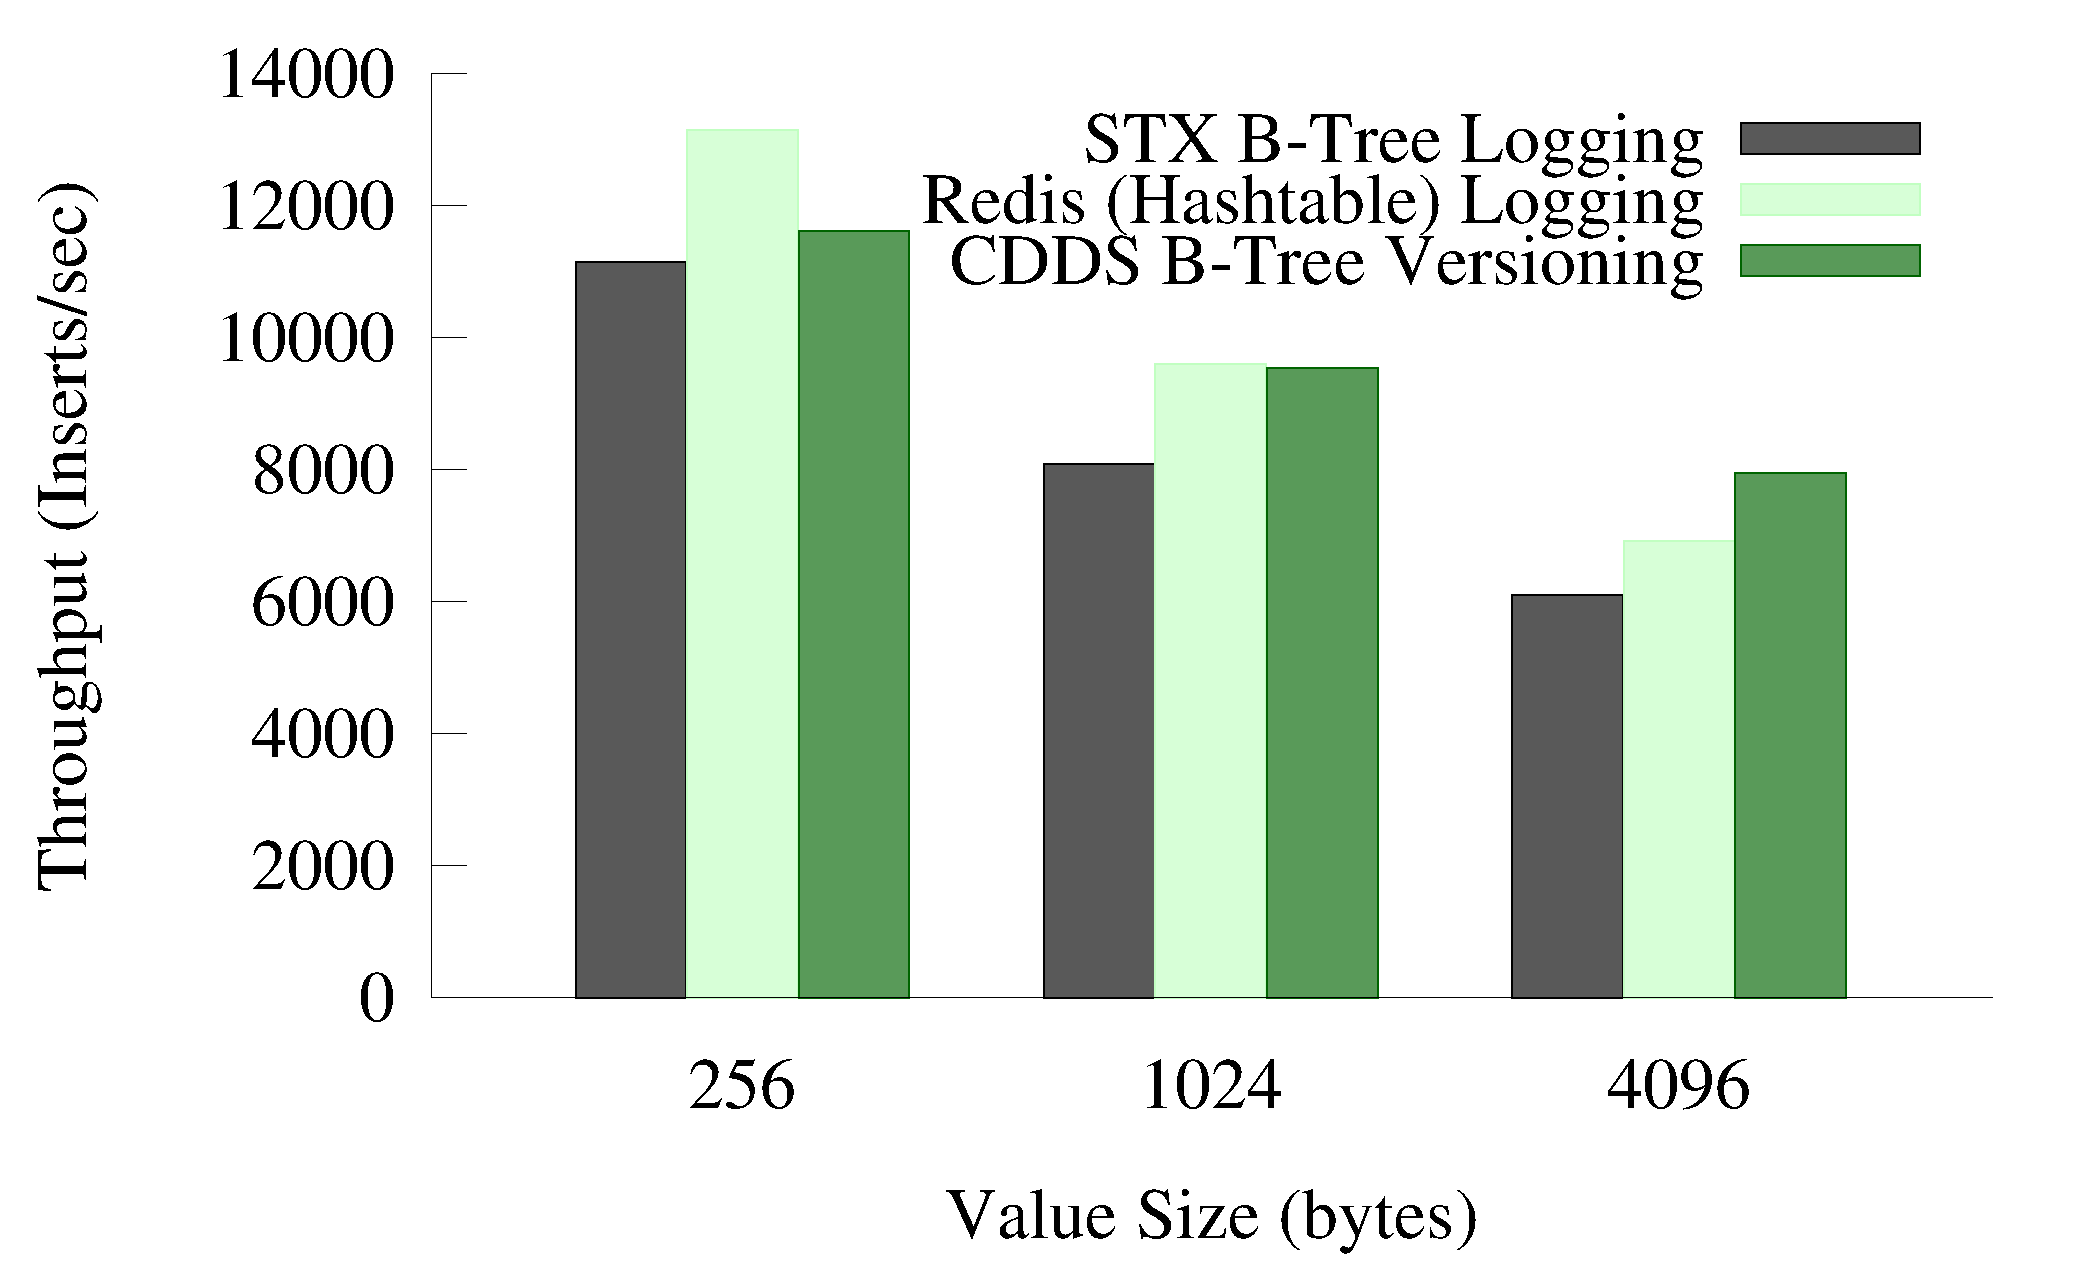
\includegraphics[width=\columnwidth]{figs/durability}
\begin{captiontext}
\centerline{Mean of 5 trials. Max.\ standard deviation: 6.7\% of the mean.}
\end{captiontext}
\captionof{figure}{Versioning vs.\ Logging}
\label{fig:durability}
\end{minipage}
\begin{minipage}[b]{0.49\textwidth}
\centerline{
\begin{tabular}{c|c}
                      & Lines of Code \\ \hline \hline
Original STX B-Tree   & 2,110         \\                 % Only include dir
CDDS Modifications    & 1,902         \\ \hline \hline
Redis (v2.0.0-rc4)               & 18,539        \\
Tembo Modifications   & 321              
\end{tabular}
}
\caption{Lines of Code Modified}
\label{tab:integration}
\end{minipage}
\end{table}




Apart from the B-Tree specific logging performed by BDB in
Chapter~\ref{sec:api_microbench}, we also wanted to compare CDDS
versioning when integrated into Tembo to the write-ahead log used by
Redis in fully-durable mode.  Redis uses a hashtable and, as it is
hard to compare hashtables and tree-based data structures, we also
replaced the hashtable with the STX B-Tree. In this single-node
experiment, we used 6~Tembo or Redis data stores and 2
clients\footnote{Being event-driven, both Redis and Tembo are
  single-threaded. Therefore one data store (or client) is run per core
  in this experiment.}.  The write-ahead log for the Redis server was
stored on an in-memory partition mounted as \texttt{tmpfs} and did not
use the hard disk. Each client performed 1M inserts over the
loopback interface.

The results, presented in Figure~\ref{fig:durability}, show that as
the value size is increased, Tembo performs up to 30\% better than
Redis integrated with the STX B-Tree.  While Redis updates the
in-memory data copy and also writes to the append-only log, Tembo only
updates a single copy.  While hashtable-based Redis is faster than
Tembo for 256~byte values because of faster lookups, even
with the disadvantage of a tree-based structure, Tembo's performance
is almost equivalent for 1~KB values and is 15\% faster for 4~KB
values.

The improvements for the experiments in this section are lower than those in
Chapter~\ref{sec:api_microbench} because of network latency overhead.  The
\texttt{fsync} implementation in \texttt{tmpfs} also does not explicitly flush
modified cache lines to memory and is therefore biased against Tembo.  We are
working on modifications to the file system that will enable a fairer
comparison.  Finally, some of the overhead is due to maintaining ordering
properties in the CDDS-based B-Tree to support range scans - a feature not used
in the current implementation of Tembo.

%one should note that Tembo does not utilize all
%features of the CDDS B-Tree, including range scans and iterator
%support.  Tembo's evaluation is therefore biased against CDDSs because
%it pays the runtime overhead for these features but does not use them.

\begin{figure}[t]
\begin{minipage}[b]{0.49\textwidth}
\centerline{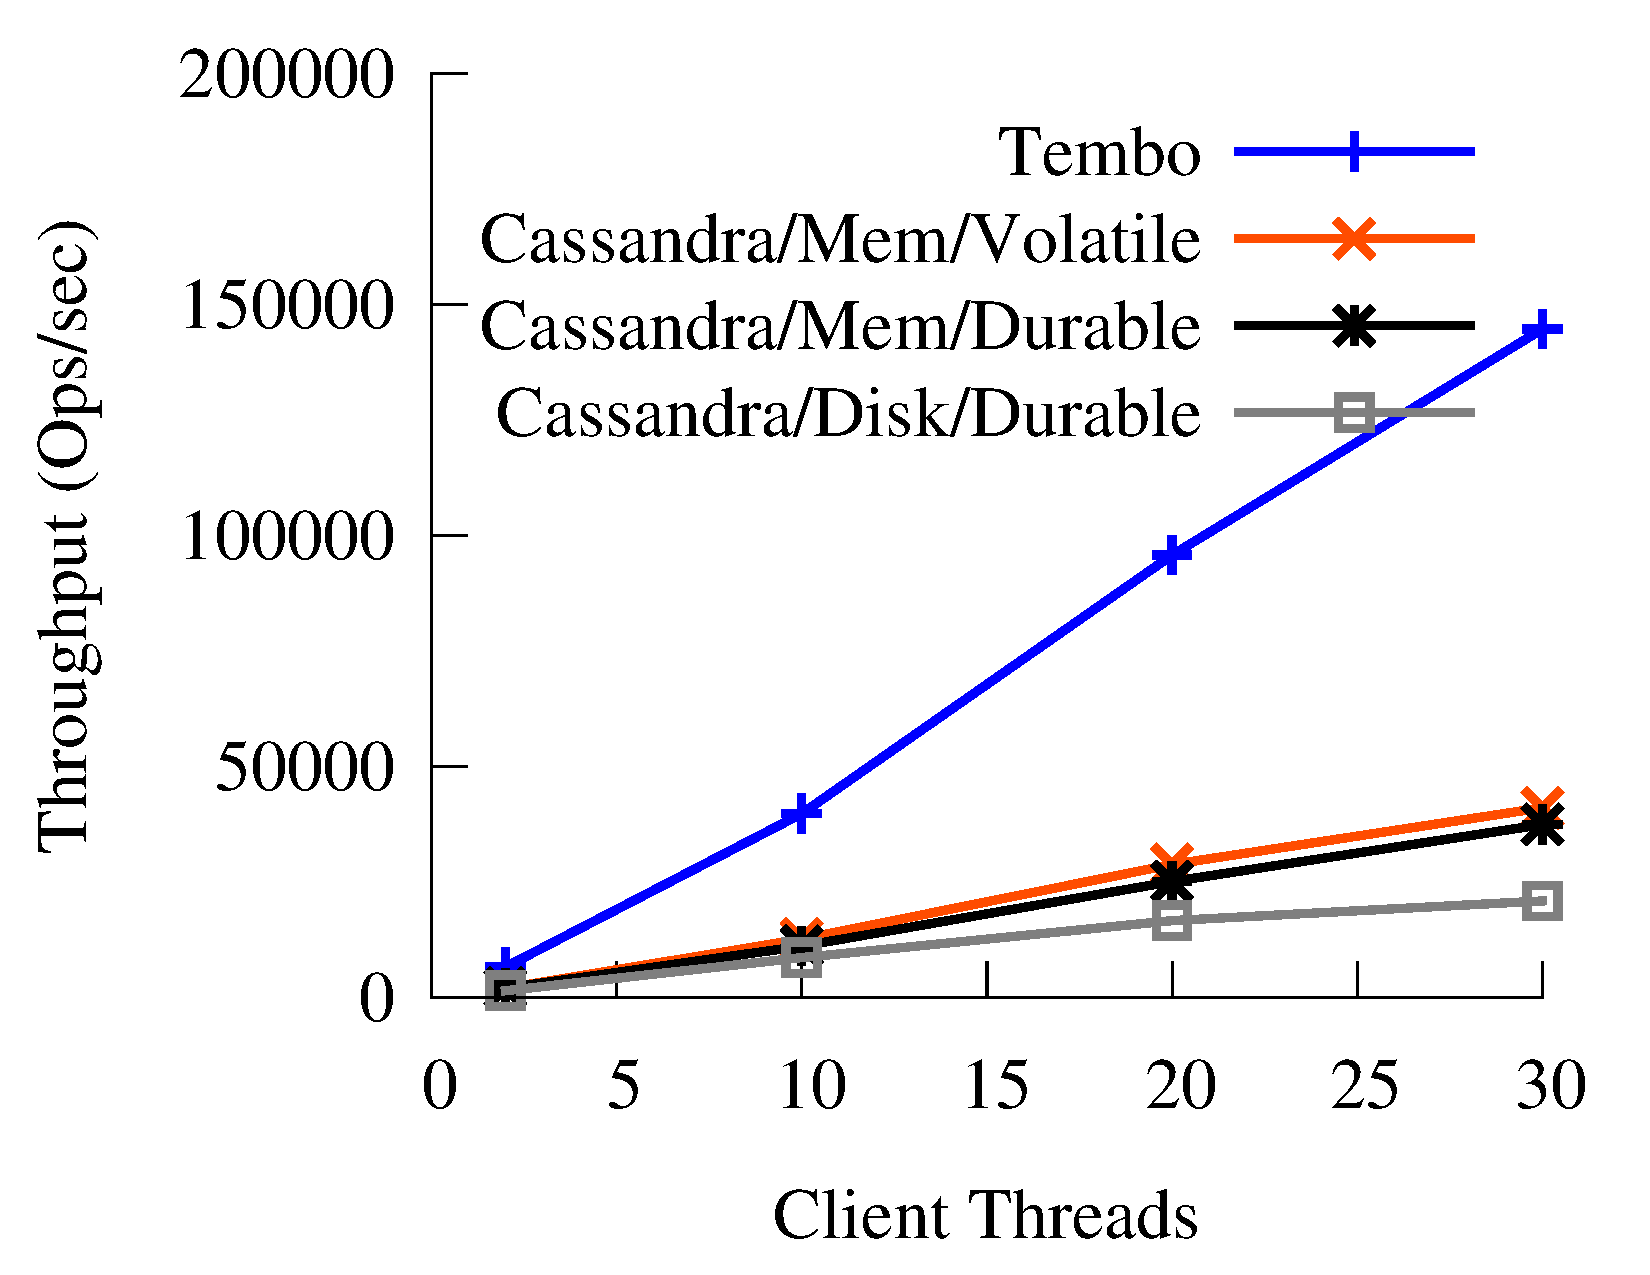
\includegraphics[width=0.85\columnwidth]{figs/ycsb-a}}
\begin{captiontext}
 \centerline{Mean of 5 trials. Max.\ standard deviation: 7.8\% of the
   mean.}
\end{captiontext}
\caption[Yahoo Cloud Serving Benchmark: SessionStore]{YCSB: SessionStore}
\label{fig:ycsb_session_store}
\end{minipage}
\begin{minipage}[b]{0.49\textwidth}
\centerline{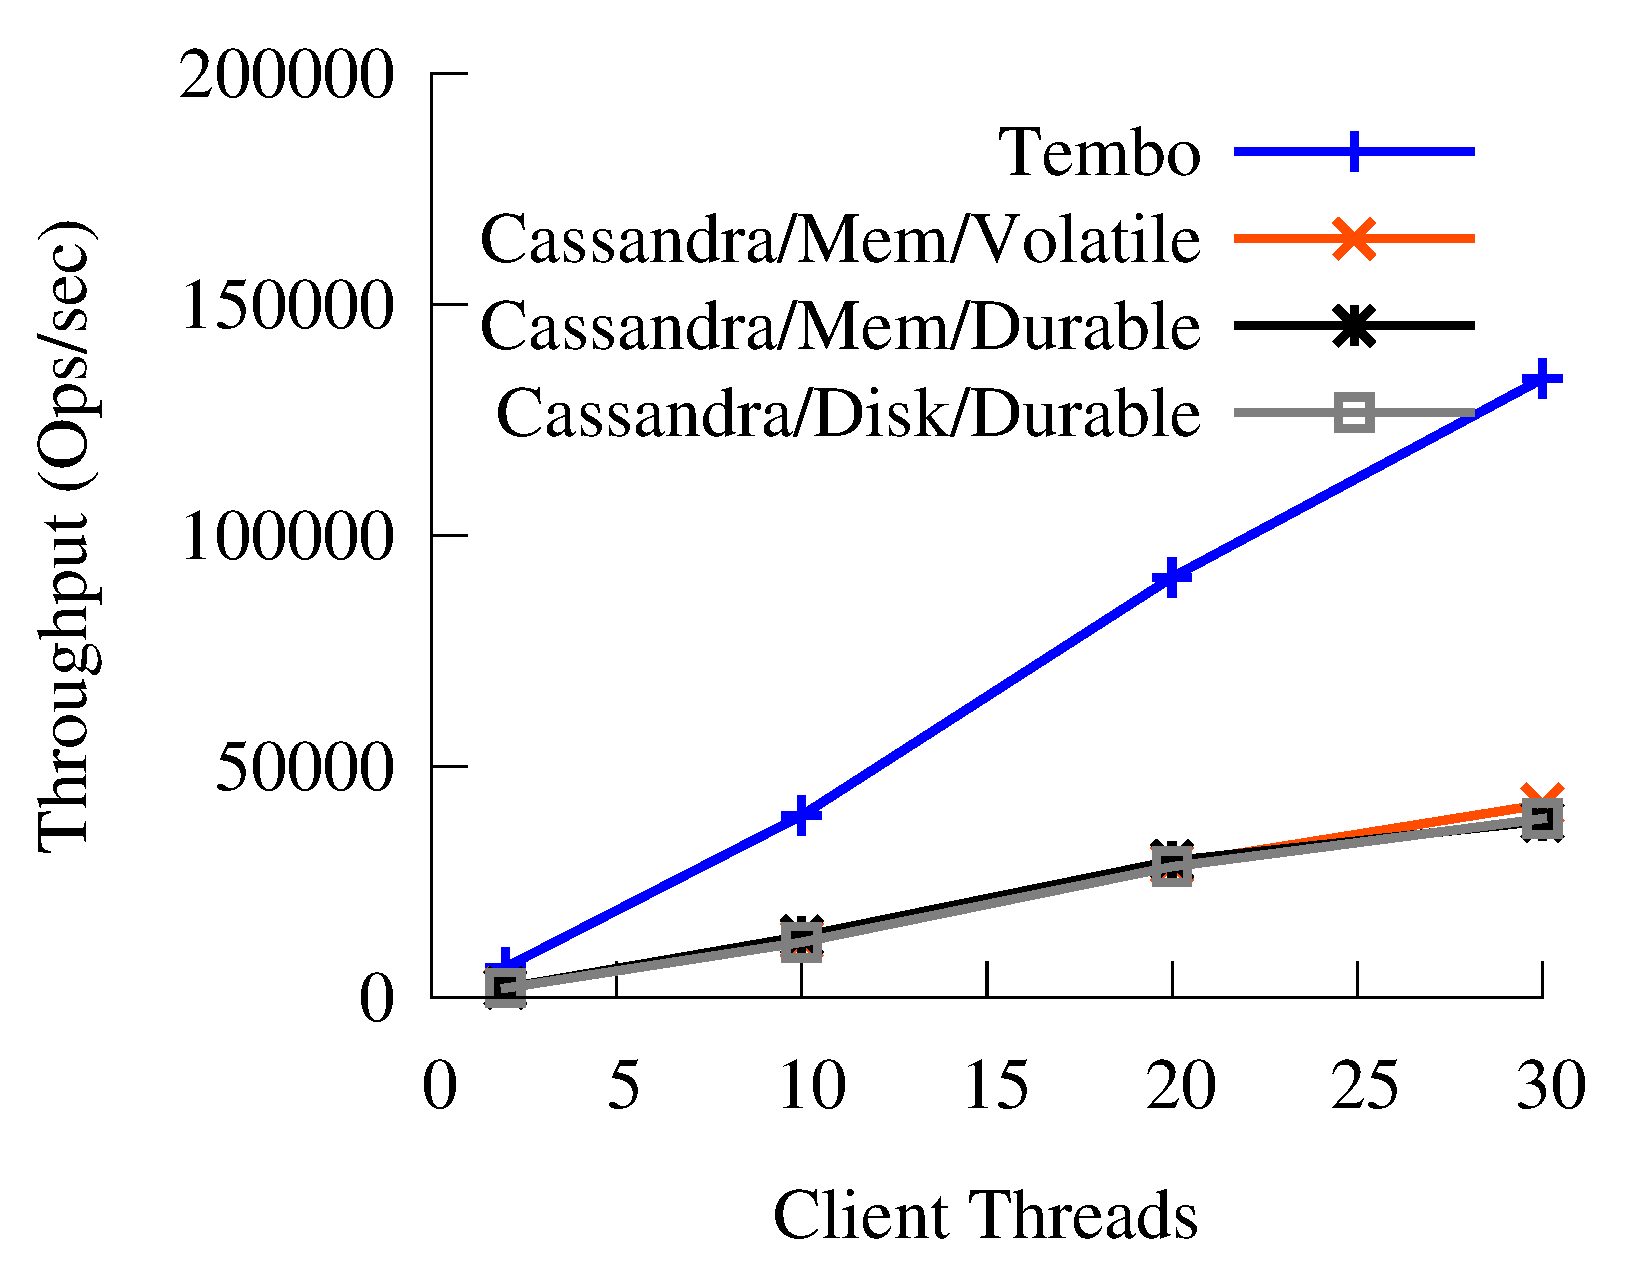
\includegraphics[width=0.85\columnwidth]{figs/ycsb-d}}
\begin{captiontext}
\centerline{Mean of 5 trials. Max.\ standard deviation: 8.1\% of the
  mean.}
\end{captiontext}
\caption[Yahoo Cloud Serving Benchmark: StatusUpdates]{YCSB: StatusUpdates}
\label{fig:ycsb_status_updates}
\end{minipage}
\end{figure}

\section{End-to-End Comparison}


For an end-to-end test, we used YCSB, a framework for evaluating the
performance of Key-Value, NoSQL, and cloud storage systems~\citep{Cooper10}.
In this experiment, we used 13 servers for the cluster and 2 servers
as the clients.  We extended YCSB to support Tembo, and present
results from two of YCSB's workloads.  Workload-A, referred to as
SessionStore in this section, contains a 50:50 read:update mix and is
representative of tracking recent actions in an online user's session.
Workload-D, referred to as StatusUpdates, has a 95:5 read:insert mix.
It represents people updating their online status (e.g., Twitter
tweets or Facebook wall updates) and other users reading them.  Both
workloads execute 2M operations on values consisting of 10 columns
with 100~byte fields.

We compare Tembo to Cassandra (v0.6.1)~\citep{Lakshman10}, a
distributed data store that borrows concepts from
BigTable~\citep{Chang08} and Dynamo~\citep{DeCandia07}.  We used three
different Cassandra configurations in this experiment.  The first two
used a ramdisk for storage but the first (Cassandra/Mem/Durable)
flushed its commit log before every update while the second
(Cassandra/Mem/Volatile) only flushed the log every 10 seconds.  For
completeness, we also configured Cassandra to use a disk as the
backing store (Cassandra/Disk/Durable).

Figure~\ref{fig:ycsb_session_store} presents the aggregate throughput
for the SessionStore benchmark. With 30 client threads, Tembo's
throughput was $286$\% higher than memory-backed durable Cassandra.
Given Tembo and Cassandra's different design and implementation
choices, the experiment shows the overheads of Cassandra's in-memory
``memtables,'' on-disk ``SSTables,'' and a write-ahead log,
vs.\ Tembo's single-level store.  Disk-backed Cassandra's throughput
was only 22--44\% lower than the memory-backed durable configuration.
The large number of disks in our experimental setup and a 512~MB
battery-backed disk controller cache were responsible for this
better-than-expected disk performance.  On a different machine with
fewer disks and a smaller controller cache, disk-backed Cassandra
bottlenecked with 10~client threads. Formal performance 
models~\cite{Varki04} designed for disk arrays have also shown the 
benefits of using battery-backed disk controller caches.

 
Figure~\ref{fig:ycsb_status_updates} shows that, for the StatusUpdates
workload, Tembo's throughput is up to 250\% higher than memory-backed
durable Cassandra.  Tembo's improvement is slightly lower than the
SessionStore benchmark because StatusUpdates insert operations update all
10 columns for each value, while the SessionStore only selects one random
column to update.  Finally, as the entire data set can be cached in
memory and inserts represent only 5\% of this workload, the different
Cassandra configurations have similar performance.


% LocalWords:  Condit NVBM AMD SAS ramdisk mfence Versioning TinySTM GC GHz DL
% LocalWords:  Hans's versioning versioned unversioned Redis YCSB Xeon  Tembo
% LocalWords:  MultCallFlushLRU clflush multi Nehalem versioning's Proliant API
% LocalWords:  NoSQL online BigTable memtables SSTables Tembo's Gigabit CDDS KV
% LocalWords:  cacheline Microbenchmark BDB tuples BDB's ing STX tradeoff HMSET
% LocalWords:  hashtable syscall tradeoffs dels sloccount lookup VTune noop STL
% LocalWords:  Oprofile Microbenchmarks Facebook SessionStore StatusUpdates UNC
% LocalWords:  bottlenecked SNP CDDSs runtime lookups loopback CDDS's YCSB's
% LocalWords:  hashtables tmpfs fsync

\chapter{Profiling and Analysis}
\label{sec:profile}

In order to compare different design choices and get a deeper understanding
of CDDS, we perform experiments using Cafegrind~\cite{Chan11}, an extension to
the Valgrind~\cite{Nethercote07} memory profiling framework. The profiler
instruments all memory accesses and memory allocations and gives
us an accurate count of the number and frequency of memory operations to heap
allocations. Moreover, since Cafegrind can also infer the types of heap
allocations, we can restrict the analysis to objects that we believe will be
stored in NVBM. By measuring the number of writes to NVBM, we can estimate the
bandwidth usage and power consumption for different configurations.
Furthermore, knowing which NVBM locations are updated frequently can help
design wear-leveling algorithms. 

\begin{figure}[t]
\begin{minipage}[b]{0.49\linewidth}
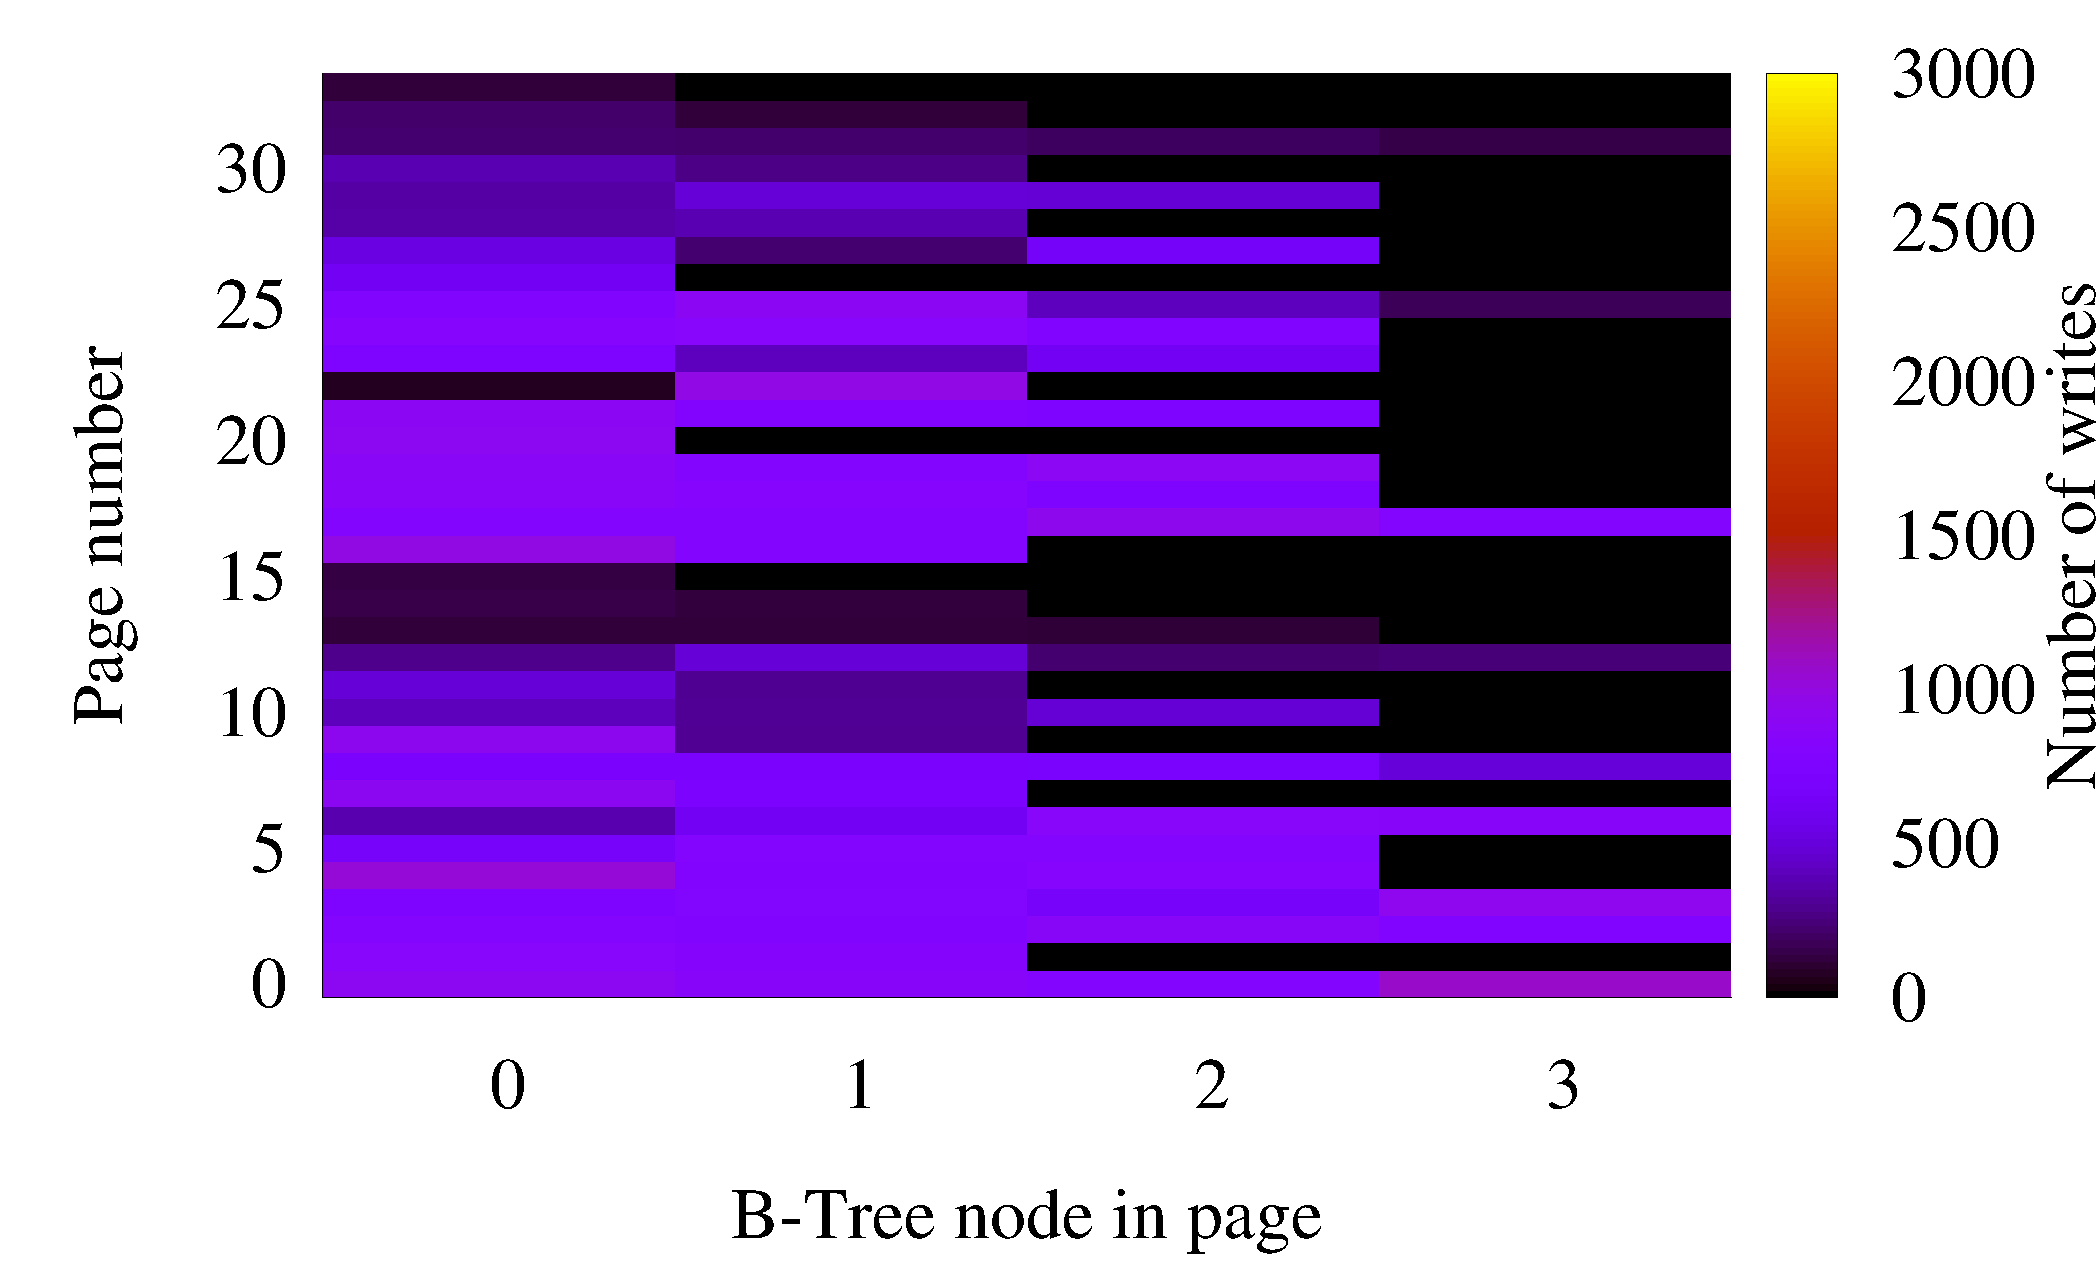
\includegraphics[width=\columnwidth]{figs/write-locations-cdds}
\caption{Heat map of writes in CDDS B-Tree}
\label{fig:write-loc-cdds}
\end{minipage}
\begin{minipage}[b]{0.49\linewidth}
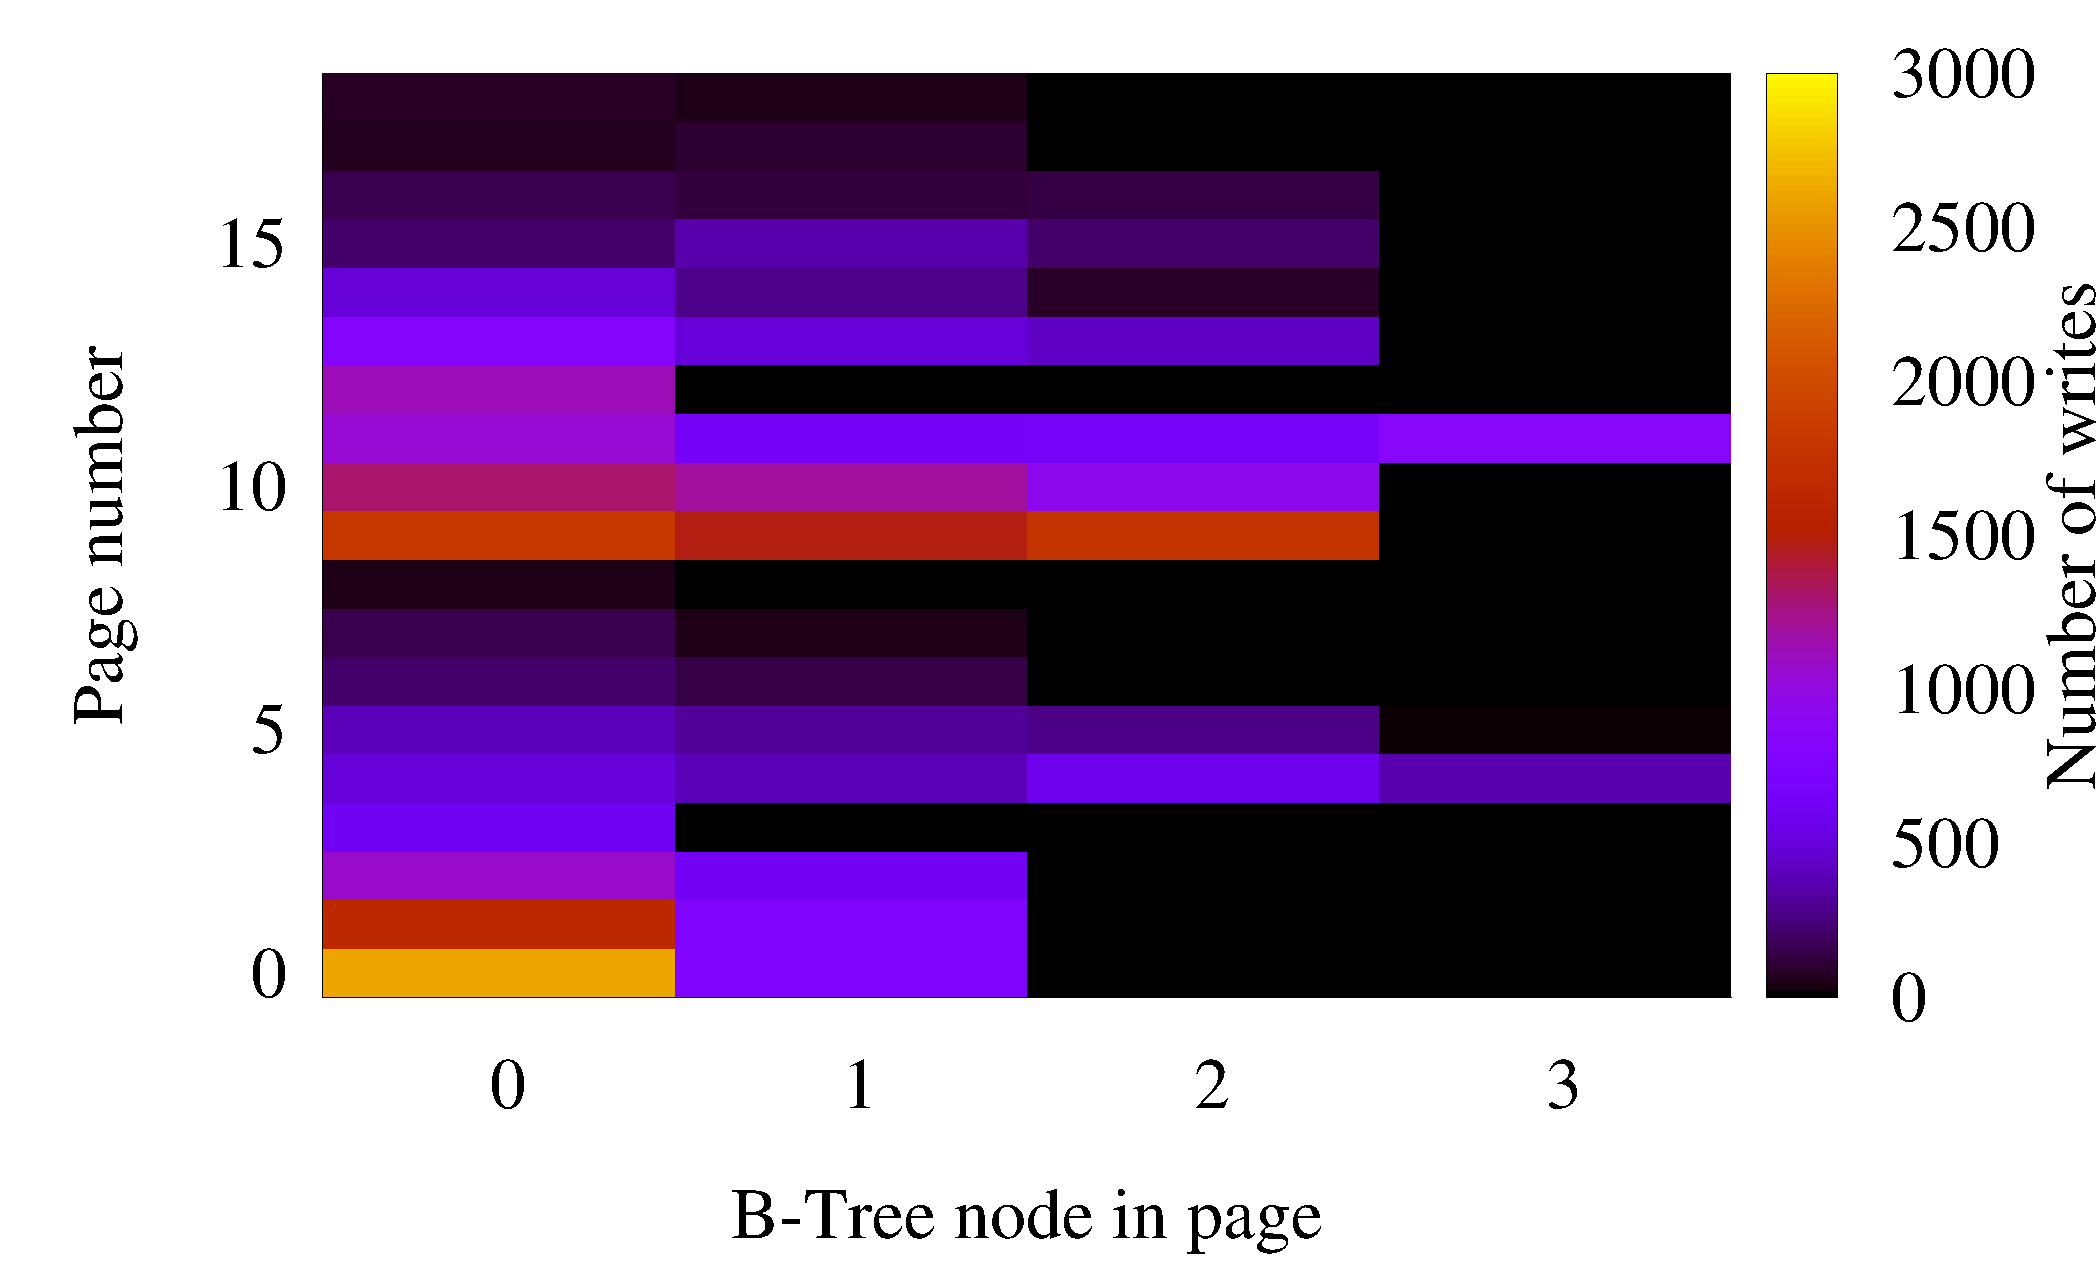
\includegraphics[width=\columnwidth]{figs/write-locations-stx}
\caption{Heat map of writes in STX B-Tree}
\label{fig:write-loc-stx}
\end{minipage}
\end{figure}

\section{Write Frequency by Location}
In order to measure how CDDS-versioning can help in wear-leveling, we profile
the number of writes made to a CDDS B-Tree and the STX B-Tree. We run the same
benchmark used in Section~\ref{sec:api_microbench} but insert only 1000 keys to
help visualize the number of writes per B-Tree node. The keys are chosen
randomly to ensure that they are evenly spread out over the key space and
repeated runs of the experiment produced similar results.  Using the type
information inferred by Cafegrind, we filter the store instructions which are
made on B-Tree nodes during execution. As seen in
Figure~\ref{fig:write-loc-cdds}, Figure~\ref{fig:write-loc-stx} the number of
writes per B-Tree node is distributed in the case of a CDDS B-Tree and there
are no hot spots. The STX B-Tree however has some hot spots which have many
more writes than other locations. It can also be seen that there are 93 B-Tree
nodes created in the CDDS B-Tree while only 47 are used in the STX B-Tree. This
includes leaf nodes and inner nodes created while inserting elements in the
workload.

\begin{figure}[t]
\begin{center}
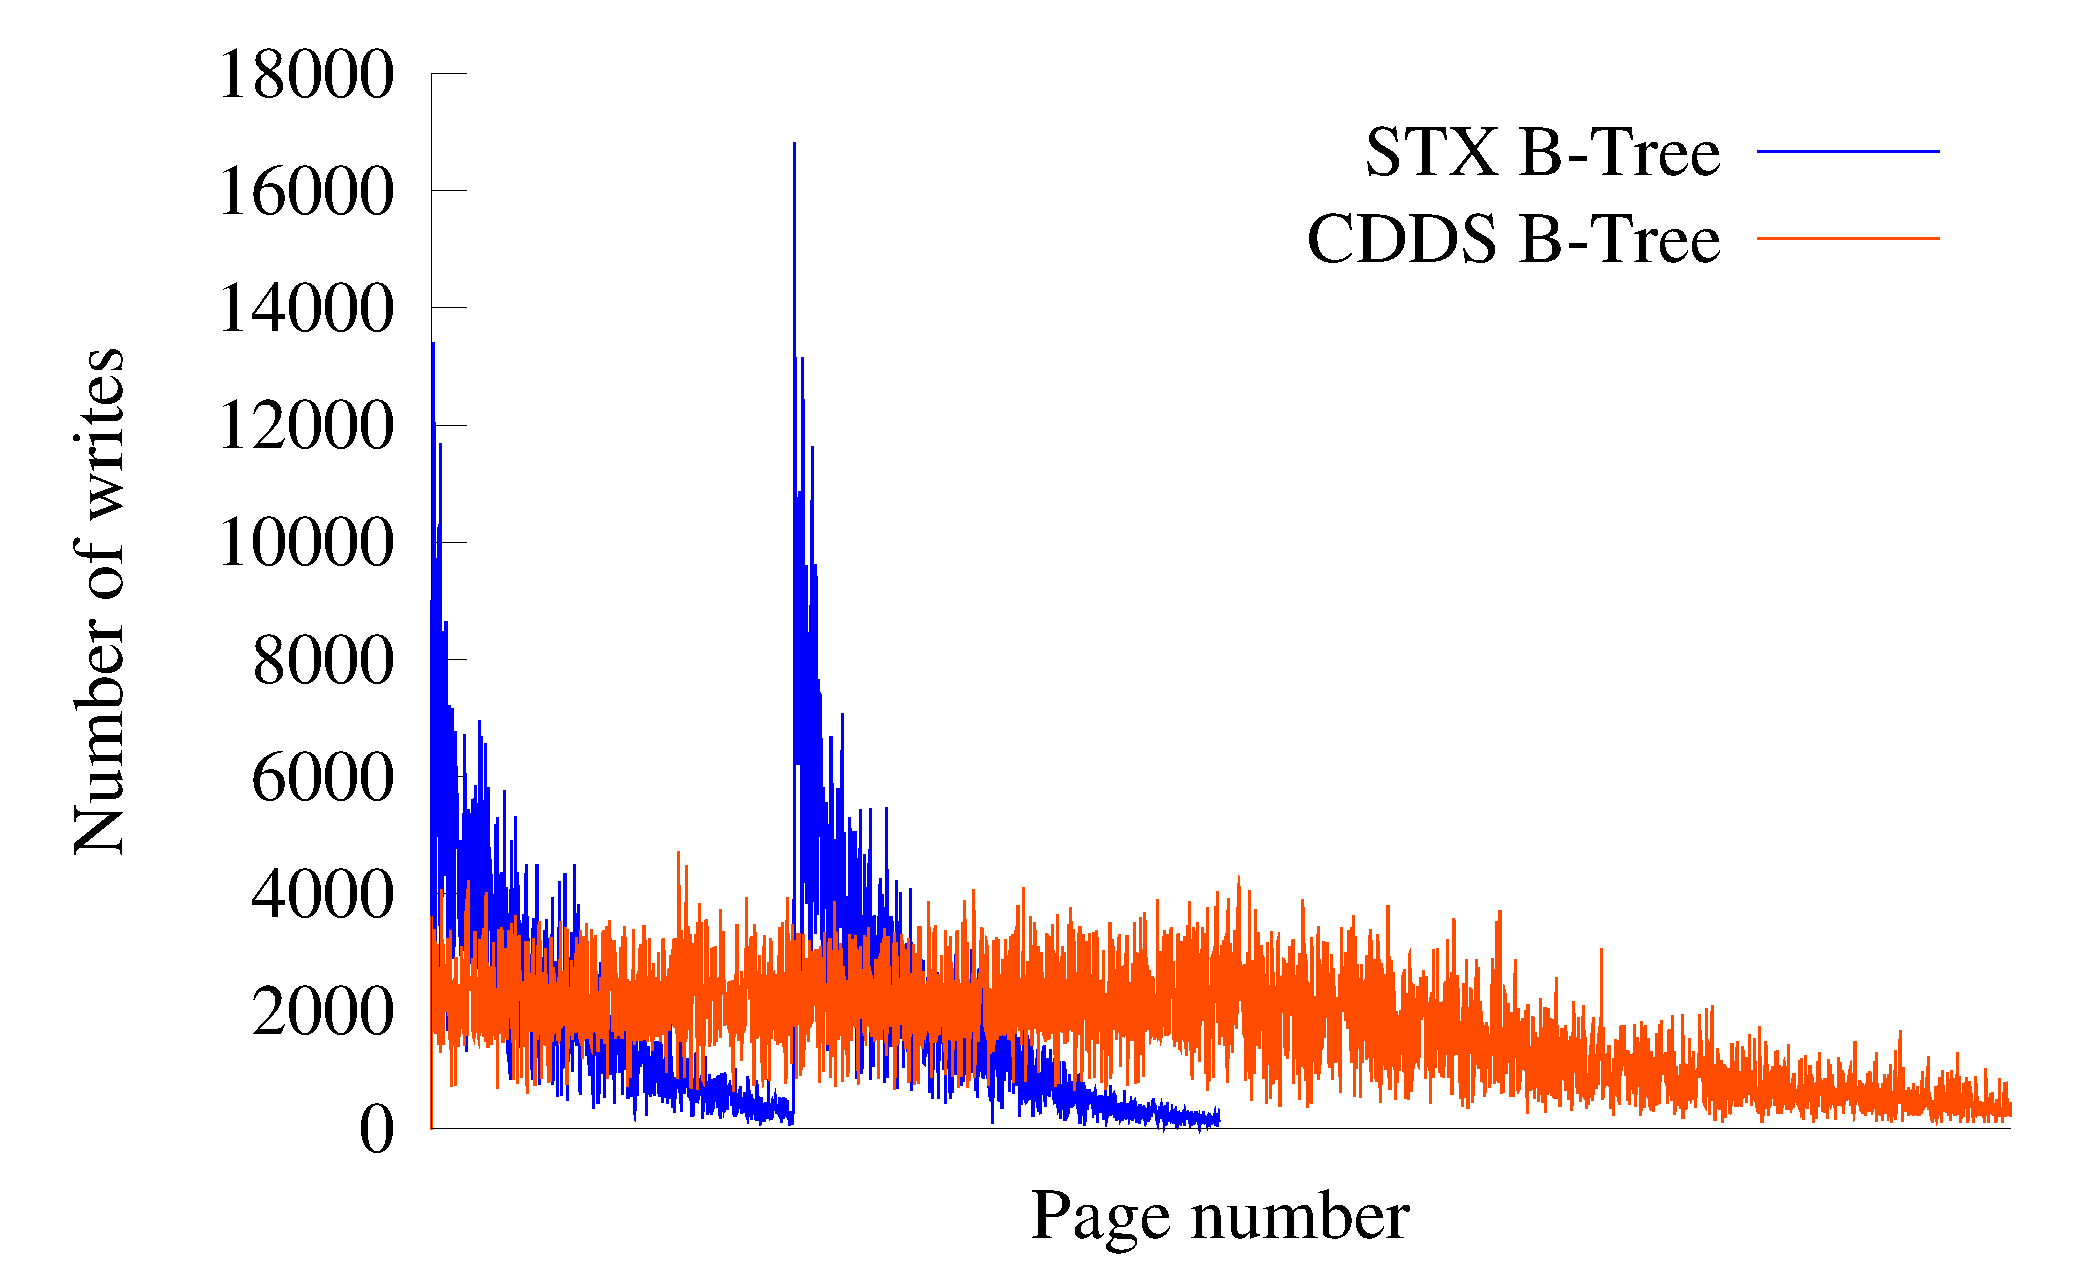
\includegraphics[width=0.7\columnwidth]{figs/wear-line}
\caption{Number of writes per page in CDDS B-Tree and STX B-Tree}
\label{fig:wear-line}
\end{center}
\end{figure}

We repeated the same experiment for a larger number of keys to see how the
number of writes per page varied across a larger number of pages. The results
from an experiment where 100K keys were inserted is shown in
Figure~\ref{fig:wear-line}. In this graph, the number of writes made to a
particular page is plotted for every page used by the application. Similar to
the previous figure, we can see that writes to a CDDS B-Tree are evenly
distributed across a larger number of pages. We can also see that in the
STX B-Tree there are some pages which have up to 16,817 writes, while other pages
have as few as 36 writes during the experiment. Hence we believe that
CDDS-based data structures can be a useful building block to design integrated
wear-leveling solutions for NVBM.
 
\begin{figure}[t]
\begin{center}
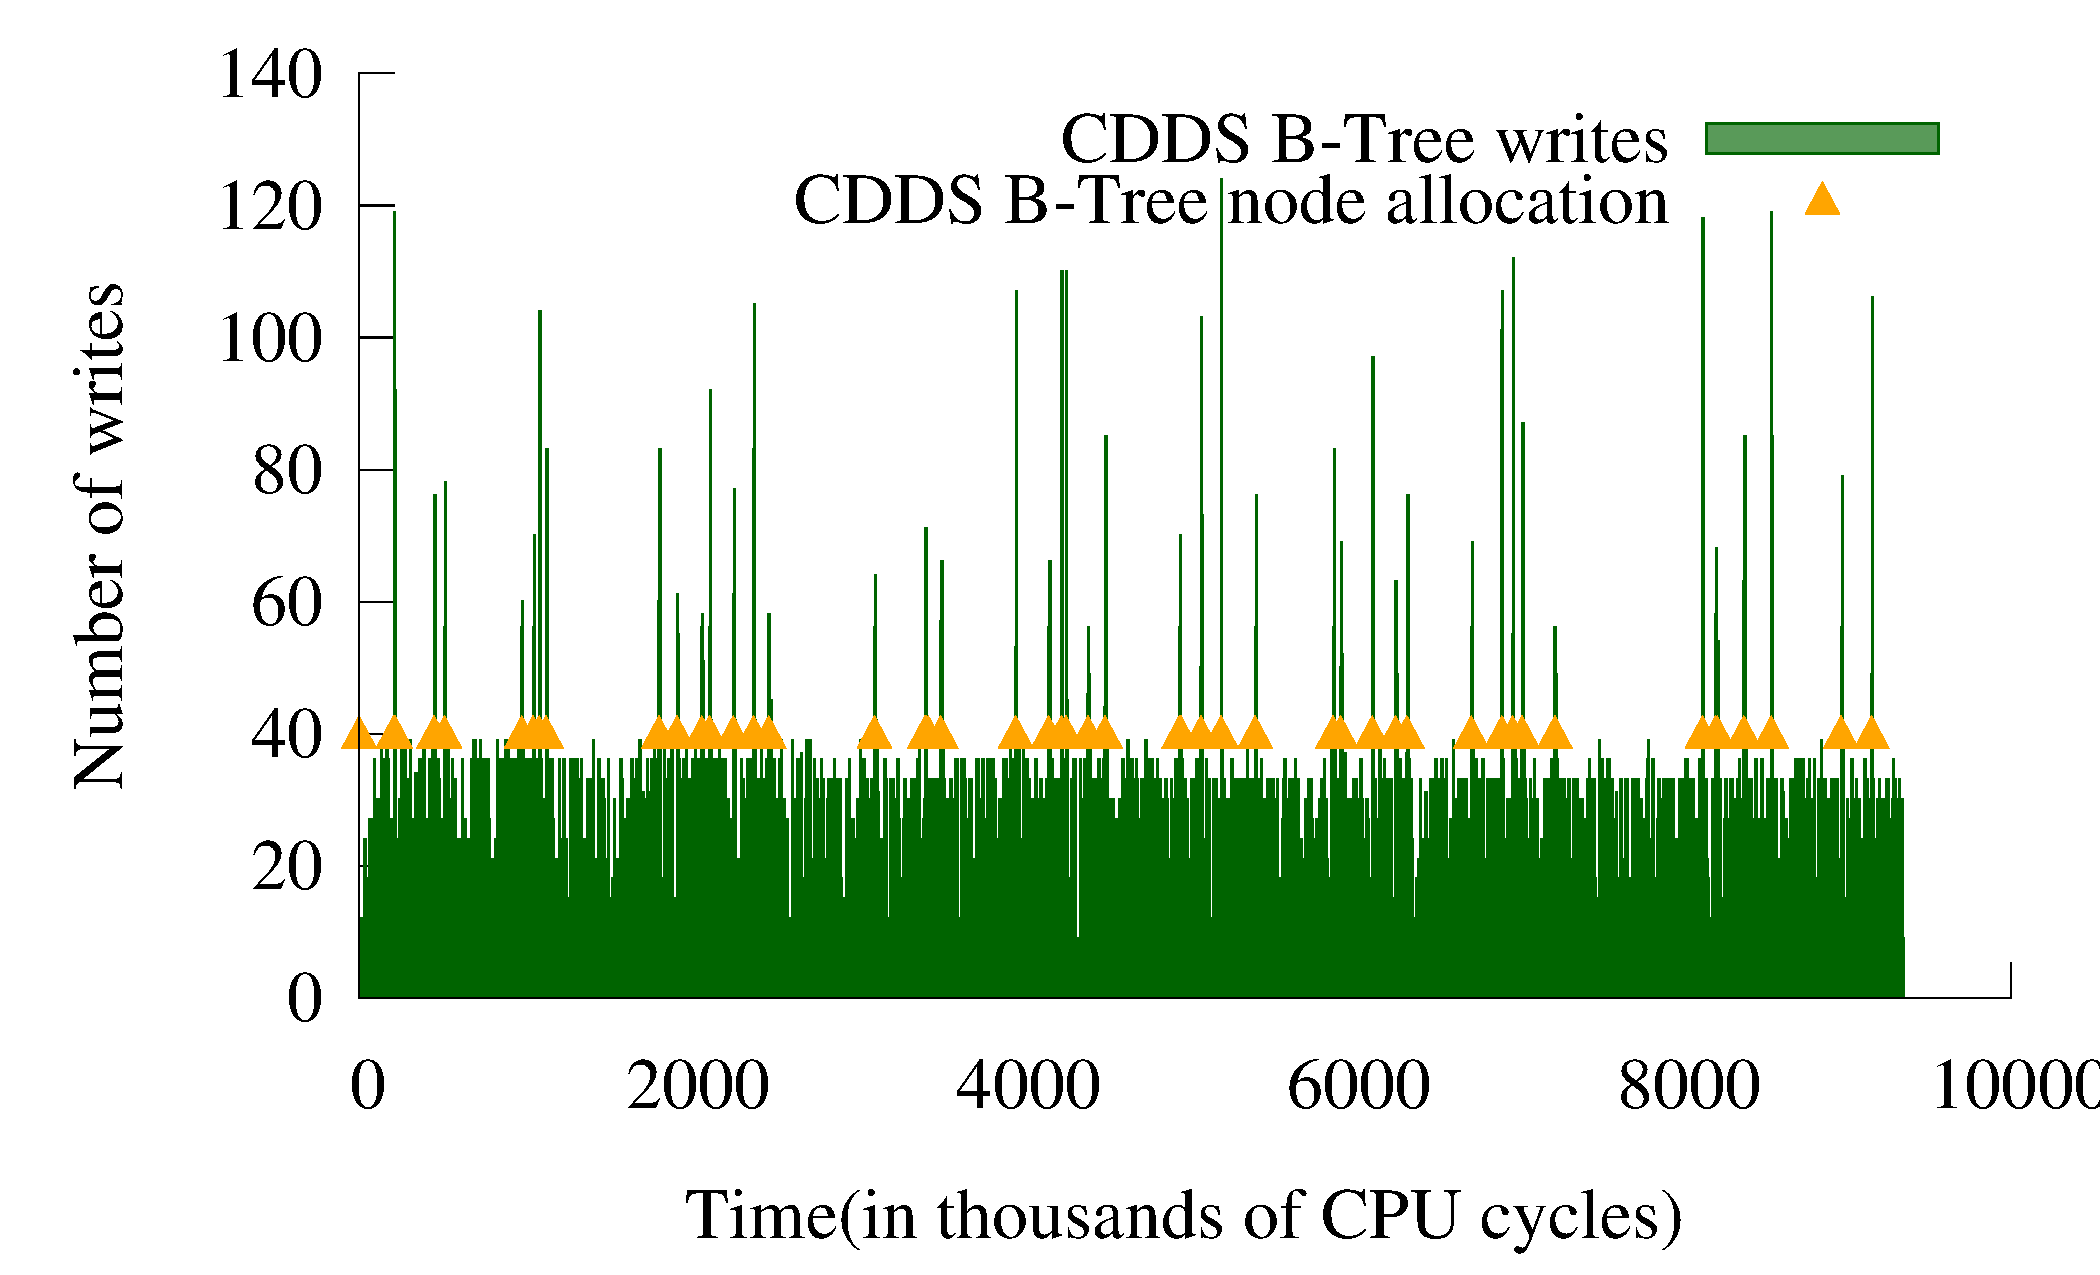
\includegraphics[width=0.7\columnwidth]{figs/write-malloc}
\caption{Writes and Memory allocation events in CDDS B-Tree}
\label{fig:write-time-cdds}
\end{center}
\end{figure}

\section{Write Frequency by Time}
Profiling the CDDS B-Tree using Cafegrind also helps us understand how many
writes are sent to NVBM over time. We can also check if there are some events
which cause a sudden increase in the number of writes. Running the same
micro-benchmark, described in the previous section, we plot the number of
writes that happen with respect to time in CPU clock cycles. In
figure~\ref{fig:write-time-cdds}, writes to B-Tree nodes are categorized into
bins, where a bin corresponds to 2000 CPU cycles. We also plot the allocation
of new B-Tree nodes in the same figure. We can see that when new nodes are
created due to a \texttt{split\_insert}, a large number of writes are made to
NVBM.

\begin{figure}[t]
\begin{center}
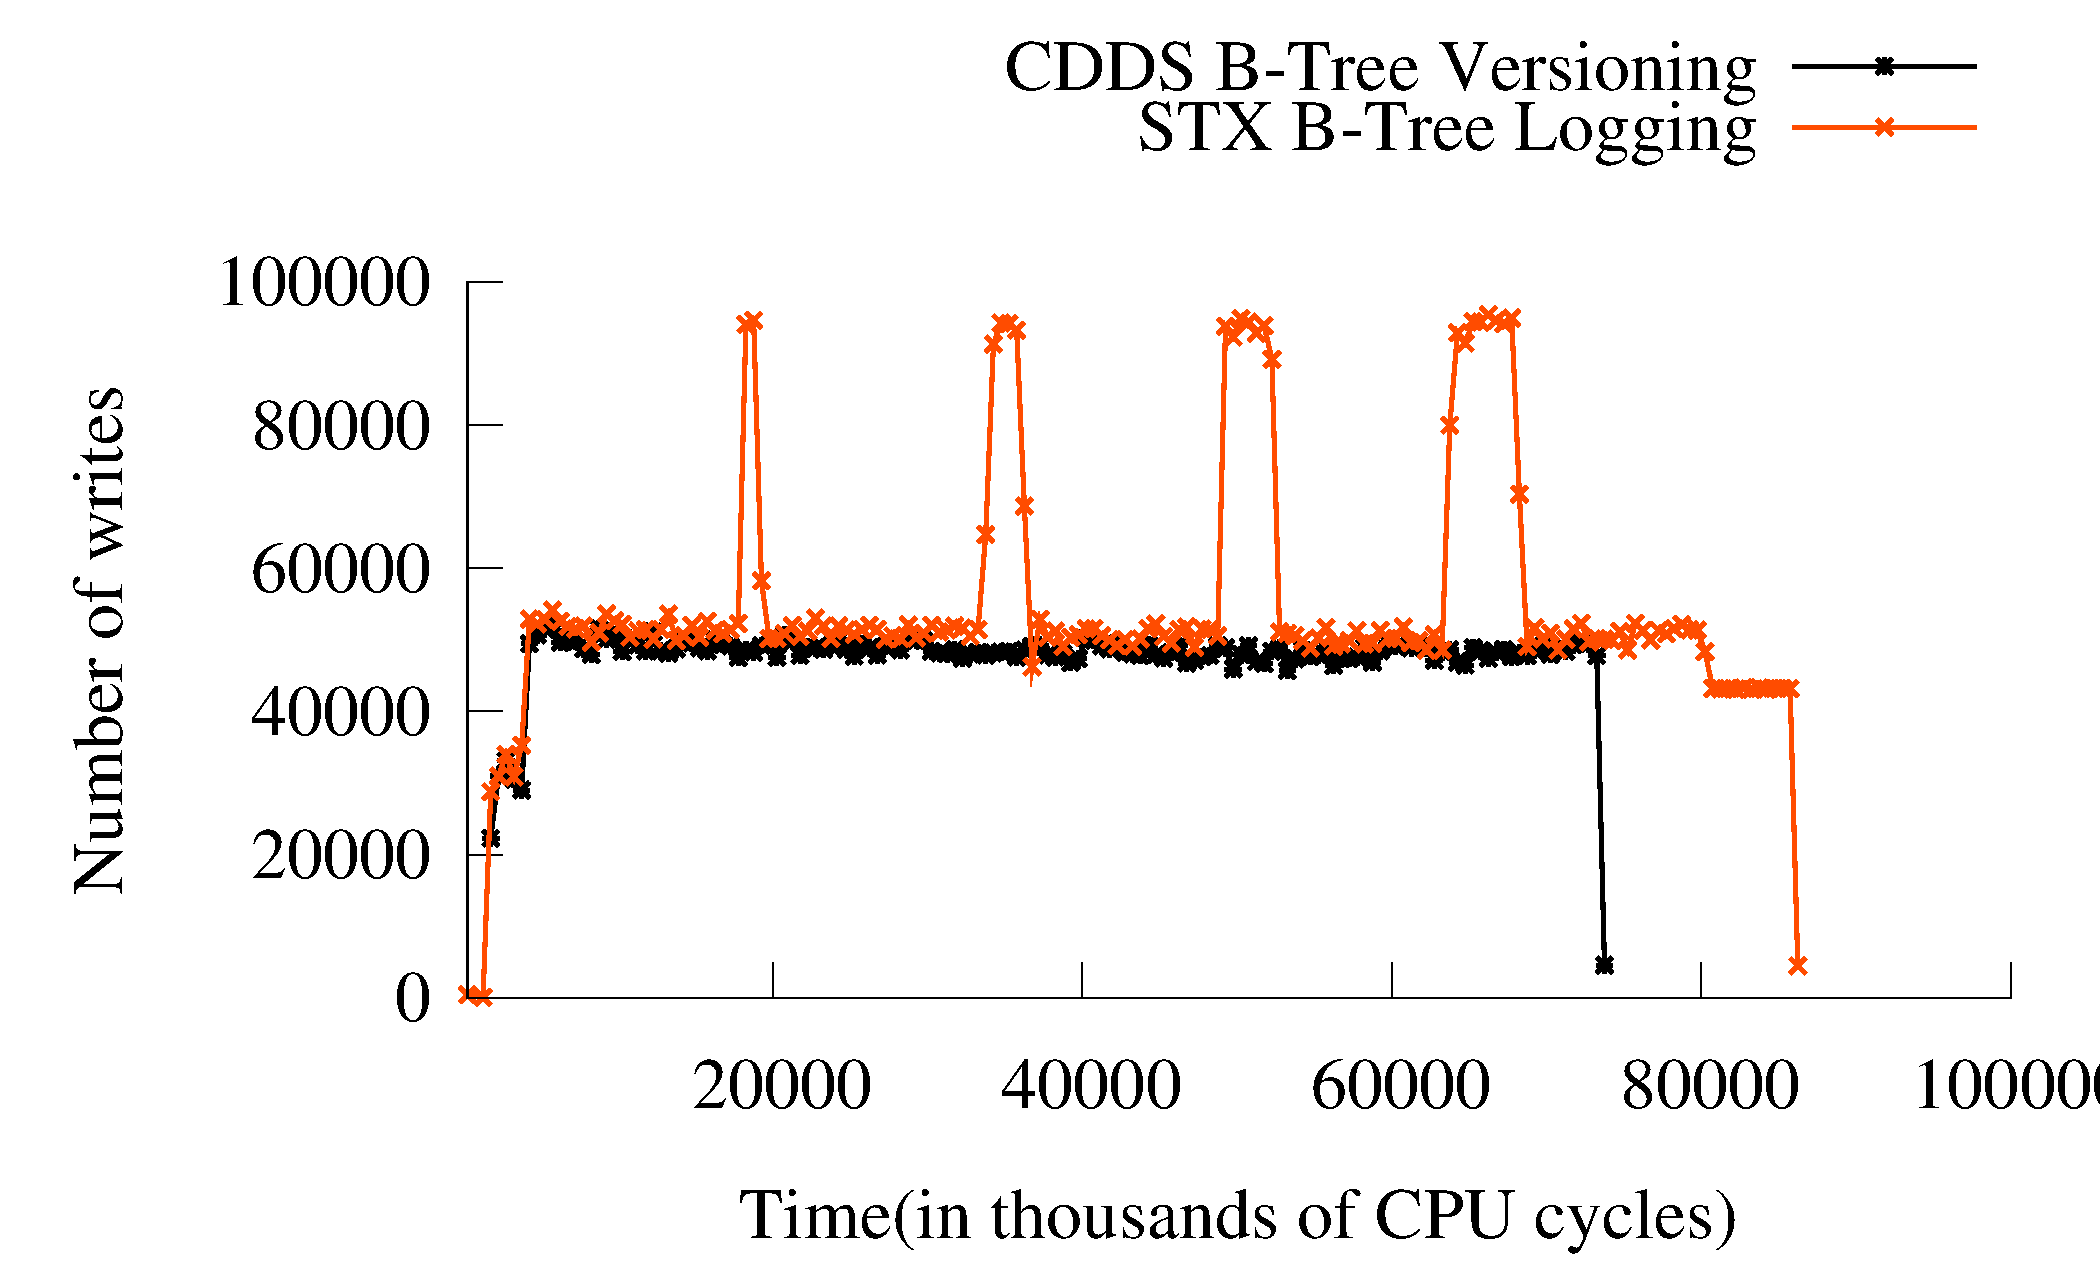
\includegraphics[width=0.7\columnwidth]{figs/write-freq}
\caption{Writes for Versioning vs.\ Logging}
\label{fig:write-freq}
\end{center}
\end{figure}

\section{Profiling Versioning vs.\ Logging}
To compare the performance of the versioning scheme used in Tembo against the
write-ahead logging scheme used in Redis we compared the throughput for both
configurations in Section~\ref{sec:versioning_logging}. Using Cafegrind, we can
gain further insight into the memory operations performed in both cases and
analyze how they affect the throughput. We repeated the experiment performed
in Section~\ref{sec:versioning_logging}, but used 10000 inserts because of the
overhead imposed by profiling. The results, shown in
Figure~\ref{fig:write-freq} show that the versioning scheme used by Tembo has
fewer writes compared to the write-ahead logging scheme. We also found that the
periodic extra writes in the write-ahead logging scheme were due to log
compaction operations. Finally we can see that the CDDS-based experiment
finishes earlier than the logging-based experiment, confirming our earlier
result in which the Tembo had a higher throughput compared to Redis.

\section{Discussion}
Although memory profiling does help us understand the behavior of CDDS, there are
some limitations to this approach. Tracing writes to NVBM locations does not 
take into account the multi-level cache design in a processor. Also, the memory
allocator and wear-leveling algorithms can change the write frequency from an
application to NVBM. However, given that NVBM is not yet commercially available,
we believe that memory profiling is a useful approach to compare different
software designs. Memory profilers can also be used to analyze how software 
systems are affected by asymmetric read/write latencies of NVBM~\cite{Qureshi10}. 


\chapter{Conclusion and Future Work}
\label{sec:conclusion}
\section{Conclusion}
AndroMEDA helps users understand the context in which their Personally Identifiable Information is used, which allows them to make more informed decisions on whether an app is action maliciously or not. 

In this paper, we introduced 3 key items:
\subsection{User-App Agreement}
%We analyze the state of Android and Permissions, and conclude the need to address the User-App Agreement, which is a framework for consenting and trusting specific actions an app may take. It lies at the heart of classifying Info Theft Malware. Android Permissions address the capabilities of an app, but fail to address the context and use of those capabilities, which are cruicial to trusting an app's actions.

We analyzed the current Android security framework: The Permission System, and found it's main flaws were it's lack of addressing context and use, which we generalize into the User-App Agreement - a framework for consenting and trusting specific actions an app may take. Whereas Android Permissions exceeded at defining general capabilities of an app, and these capabilities go a long way in shaping the User-App Agreement, they fail at addressing the context in which the permissions are used, and what they are used for.

\subsection{\temp{AndroidMarketDB}}
To perform a full analysis of the current state of Android Permissions, we use a novel dataset, \temp{AndroidMarketDB}. By analyzing more than 80\% of apps in the Google Play Store, we are able to better understand the interrelationship of permissions and expected behavior. We produce key insights as to the popularity of apps vs their PII permissions, and when apps deviate from their expected behavior - potentially violating the User-App Agreement. We then analyze a comprehensive malware dataset using the same techniques, and find that many types of malware can be identified purely by it's permission fingerprint. We conclusively show the connection between Permissions and Expected Behavior are present, but not strong enough to differentiate between Info Theft Malware and many popular apps.

\subsection{AndroMEDA}
Building off the concept of the User-App Agreement, we introduce AndroMEDA. Key parts of the User-App Agreement were previously unnoticable to the user until AndroMEDA. By giving the user more information on the context and use of permissions, they can evaluate whether they trust those actions, and ultimately whether the app is acting maliciously or not. This, in turn, helps mitigate Info Theft Malware on Android.

\section{Future Work}
\label{sec:futurework}
AndroMEDA is, ultimately, not a silver bullet at detecting all Android malware. Projects like TaintDroid and TISSA provide functionality that would greatly enhance the abilities of AndroMEDA to visualize context and use of permissions to the user, and allow them to take action against it. 

AndroMEDA could also benefit greatly from the probablistic modeling of pBMDs and Crowdroid, in correlating user action with permission behavior. These would not replace the need to alert the user, but rather be able to better dictate when to put different classes of alerts to the user, as ultimately the decision of what is malware is up to them.

The weath of data in \temp{AndroidMarketDB} was also not fully explored. We are currently interested in seeing if specific keywords in user reviews correlate with malicious software, or other problematic apps. Many more areas of metadata, like the description, developer, etc, can be further explored, to see if it gives additional insight into the nature of malware on Android.

\appendix*

%\include{Appendix.tex}

\backmatter

\bibliographystyle{abbrvnat}
%\bibliographystyle{latex8}
\bibliography{ref}

\end{document}
\endinput
%% End of file `thesis-ex.tex'.
